\documentclass%
%[handout]%
{beamer}

\mode<presentation>
{
\useinnertheme{rounded}
\useoutertheme{infolines}
\usecolortheme{orchid}
\usecolortheme{whale}
}
%\setbeamertemplate{footline}{%
%  \raisebox{5pt}{\makebox[\paperwidth]{\hfill\makebox[10pt]{\scriptsize\insertframenumber}}}}

\usepackage[english]{babel}
\usepackage[latin1]{inputenc}
\usepackage{times}
\usepackage{../example-templates}
\usepackage{../pstricks-commands}
% psfrag needed for including latex labels on eps files created with xfig


\usepackage[T1]{fontenc}
% Or whatever. Note that the encoding and the font should match. If T1
% does not look nice, try deleting the line with the fontenc.

\graphicspath{{../../modules/}}

\newcommand{\currentLecture}{4}

\newcommand{\lect}[4]{
\ifnum#3=\currentLecture
  \date{#1}
  \lecture[#1]{#2}{#3}
#4
\else
%include nothing
\fi
}

\setbeamertemplate{footline}
{
  \leavevmode%
  \hbox{%
  \begin{beamercolorbox}[wd=.333333\paperwidth,ht=2.25ex,dp=1ex,center]{author in head/foot}%
    \usebeamerfont{author in head/foot}\insertshortauthor
  \end{beamercolorbox}%
  \begin{beamercolorbox}[wd=.333333\paperwidth,ht=2.25ex,dp=1ex,center]{title in head/foot}%
    \usebeamerfont{title in head/foot}\insertshorttitle
  \end{beamercolorbox}%
  \begin{beamercolorbox}[wd=.333333\paperwidth,ht=2.25ex,dp=1ex,center]{date in head/foot}%
    \usebeamerfont{date in head/foot}\insertshortdate{}
  \end{beamercolorbox}}%
  \vskip0pt%
}

\setbeamertemplate{navigation symbols}{}


\renewcommand{\Arcsin}{\arcsin}
\renewcommand{\Arccos}{\arccos}
\renewcommand{\Arctan}{\arctan}
\renewcommand{\Arccot}{\text{arccot\hspace{0.03cm}}}
\renewcommand{\Arcsec}{\text{arcsec\hspace{0.03cm}}}
\renewcommand{\Arccsc}{\text{arccsc\hspace{0.03cm}}}


% If you have a file called "university-logo-filename.xxx", where xxx
% is a graphic format that can be processed by latex or pdflatex,
% resp., then you can add a logo as follows:

%\pgfdeclareimage[height=0.8cm]{logo}{bluelogo}
%\logo{\pgfuseimage{logo}}

\begin{document}

\AtBeginLecture{%

\title[\insertlecture]{Math 141}
\subtitle{\insertlecture}
\author[Math 141]{Catalin Zara  \\~\\\small{with modifications by  Todor Milev}\normalsize}
\institute[UMass Boston]{University of Massachusetts Boston}
\date{\insertshortlecture}
\begin{frame}
  \titlepage
\end{frame}

\begin{frame}{Outline}
  \tableofcontents[pausesections]
\end{frame}
}%

% begin lecture
\lect{2014}{Lecture  1}{1}{

%  introduction
%	coordinates

\begin{frame}
  \frametitle{Goals}

  \pause

    \begin{itemize}
      \item Understand the fundamental concepts of multivariable calculus \\

      \pause

      \item Demonstrate ability to use calculus to solve problems \\

      \pause

      \begin{itemize}
        \item Construct mathematical model \\

        \item Recognize concepts and techniques \\

        \item Apply formulas and results \\

        \item Interpret and communicate the results \\
      \end{itemize}

      \pause

      \item Build and improve portable skills\\

      \pause

      \begin{itemize}
            \item Analyze data
            \item Reason deductively
            \item Think abstractly
            \item Think analytically
            \item Think critically
            \item Solve problems
      \end{itemize}

      \pause

      \item Appreciate the beauty and power of mathematics \\

      \pause

      \item Have fun!
    \end{itemize}

\end{frame}


\begin{frame}
  \frametitle{Expectations}

  \pause

  \begin{itemize}
    \item Motivated students

    \pause

    \item Adequate background

    \pause

    \item Committed to learning

    \pause

    \item Actively involved

    \pause

    \item Able to work in groups

    \pause

    \item Secure enough to ask for help
  \end{itemize}

  \pause

  \begin{center}
    {\Huge Your expectations?}
  \end{center}

\end{frame}

\begin{frame}
  \frametitle{Functions}

  \begin{itemize}
    \item From $\RR$ to $\RR$
    \begin{itemize}
      \item Precalculus
      \item Calculus I and II
    \end{itemize}

    \pause

    \item From $\RR^{1,2,3}$ to $\RR^{1,2,3}$, all combinations
    \begin{itemize}
      \item Calculus III: Multivariable and Vector Calculus
    \end{itemize}

    \pause

    \item From $\RR^m$ to $\RR^n$
    \begin{itemize}
      \item Linear Algebra (M260)  linear case
      \item Analysis on Manifolds  general case
    \end{itemize}
  \end{itemize}

\end{frame}

\begin{frame}
\frametitle{Outline}

\begin{itemize}
  \item Part 1: Space
  \begin{itemize}
    \item Coordinate Systems
    \item Vectors
    \item Geometry: Lines and Planes
  \end{itemize}

  \item Part 2: Differentiation
    \begin{itemize}
      \item Parametric Curves
      \item Functions of Several Variables
      \item Partial Derivatives
    \end{itemize}
    
  \item Part 3: Applications of Partial Derivatives
    \begin{itemize}
      \item Optimization
      \item Parametric Surfaces, Constrained Optimization
    \end{itemize}
    
  \item Part 4: Integration
    \begin{itemize}
      \item Double Integrals
      \item Triple Integrals
    \end{itemize}
    
  \item Part 5: Vector Analysis
    \begin{itemize}
      \item Line and Surface Integrals
      \item Fundamental Theorems of Calculus
    \end{itemize}
\end{itemize}
\end{frame}



}

% begin lecture
\lect{2014}{Lecture  2}{2}{
\section{Space}

\begin{frame}
\frametitle{Space}
\begin{itemize}
\item<1-> Some subsets of points in space are special/distinguished.
\begin{itemize}
\item<2-> Lines.
\item<3-> Planes.
\end{itemize}
\item<4-> We rely on intuition rather than axiomatic construction.
\item<5-> Given a pair of objects (lines or planes), we discuss all possible configurations with respect to: 
\begin{itemize}
\item<6-> inclusion
\item<7-> intersection
\item<8-> parallelism
\item<9-> being contained in a single plane (being ``co-planar'').
\end{itemize}
\end{itemize}
\end{frame}


\begin{frame}
\frametitle{Example}

%
\begin{figure}[h]
  \psfrag{A}{$A$} 
  \psfrag{B}{$B$} 
  \psfrag{C}{$C$} 
  \psfrag{D}{$D$}  
  \psfrag{E}{$E$} 
  \psfrag{F}{$F$}  
  \psfrag{G}{$G$}   
  \psfrag{L1}{$L_1$} 
  \psfrag{L2}{$L_2$} 
  \psfrag{L3}{$L_3$}  
  \psfrag{L4}{$L_4$} 
  \psfrag{cP}{$\cP$}     
  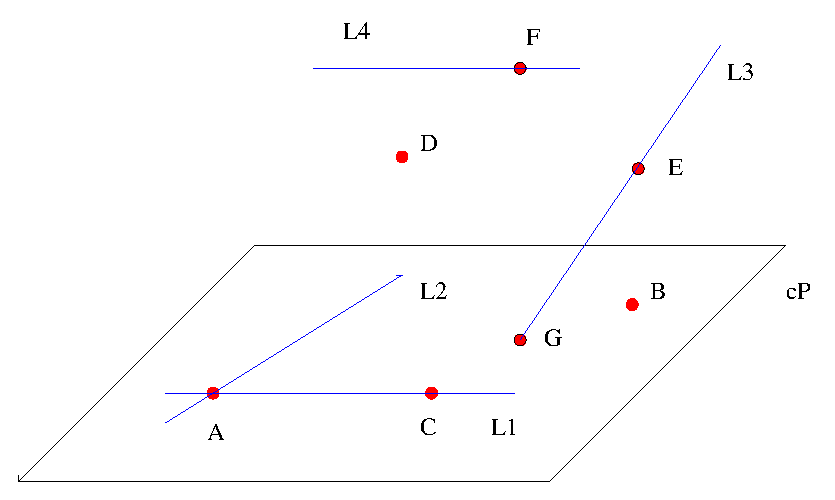
\includegraphics[height=2in]{../../modules/coordinate-systems/pictures/line_plane.eps}
  \caption{Points, lines, and planes}
  \label{fig:points_lines_planes}
\end{figure}
%
\end{frame}
\begin{frame}
 \frametitle{Distance}

\begin{itemize}
 \item Euclidean Plane: \\
    Through a point $P$ outside a line $L$\\ there passes at most one line $\ell$ parallel to $L$
  \item<2-> Distance - Primordial concept \\
      Quantifies/Measures how close/far apart are any two points \\
      $$d(A,B) = |AB|$$
  \item<3-> Measures of angles $\to$ Perpendicularity
      \begin{itemize}
	\item Line and Line
        \item Line and Plane
        \item Plane and Plane
      \end{itemize}
  \end{itemize}

\end{frame}
\begin{frame}
%
\begin{figure}[h]
  \psfrag{cP1}{$\mathcal{P}_1$}
  \psfrag{cP2}{$\mathcal{P}_2$}
  \psfrag{L1}{$L_1$}
  \psfrag{L2}{$L_2$}
  \psfrag{L}{$L$}  
  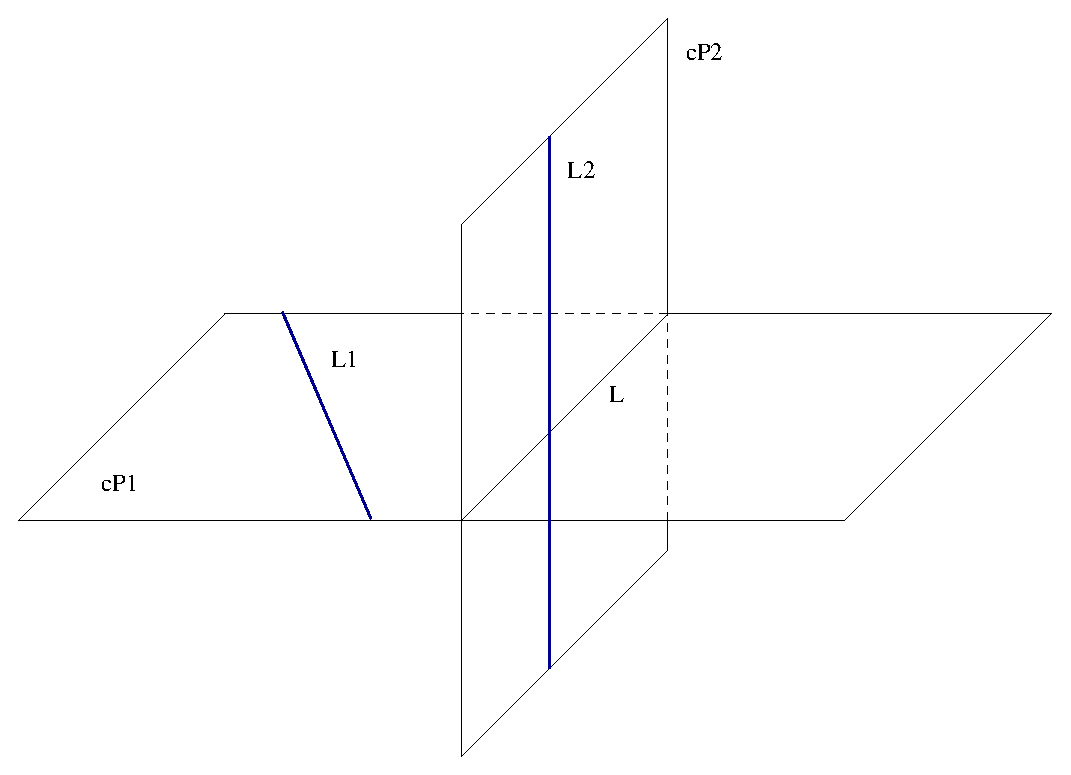
\includegraphics[height=2in]{./images/perpendicularity.eps}
  %\caption{Perpendicularity}
  \label{fig:perpendicularity}
\end{figure}
%
\begin{itemize}
%
\item The planes $\mathcal{P}_1$ and $\mathcal{P}_2$ are perpendicular on each other;
%
\item The lines $L_2$ and $L$ are coplanar and perpendicular on each other;
%
\item The lines $L_1$ and $L_2$ are skew but perpendicular on each other;
%
\item The lines $L_1$ and $L$ are coplanar and not perpendicular;
%
\item The line $L_2$ is perpendicular to the plane $\mathcal{P}_1$;
%
\item The line $L_1$ is not perpendicular to the plane $\mathcal{P}_2$.
\end{itemize}

\end{frame}
%\begin{comment}
\begin{frame}
\frametitle{Rectangular/Cartesian Coordinates}
\begin{columns}
\column[t]{0.3\textwidth}
\psset{xunit=0.7cm, yunit=0.7cm}
\begin{pspicture}(-0.5 ,-2)(4.5, 4)
\fcBoundingBox{-0.5}{-2}{4.5}{4}
\tiny
\uncover<3->{
\fcLineIIId{[0 0 0]}{[3 0 0]}
\fcLineIIId{[0 0 0]}{[0 3 0]}
\fcLineIIId{[0 0 0]}{[0 0 3]}
}
\uncover<4->{
\fcLineIIId[arrows=->]{[0 0 0]}{[3 0 0]}
\fcLineIIId[arrows=->]{[0 0 0]}{[0 3 0]}
\fcLineIIId[arrows=->]{[0 0 0]}{[0 0 3]}
}
\uncover<5->{
\fcPutIIId[t]{[3 0 0]}{\alertNoH{5}{$x$}}
\fcPutIIId[lb]{[0 3 0]}{\alertNoH{5}{$y$}}
\fcPutIIId[b]{[0 0 3]}{\alertNoH{5}{$z$}}
}
\uncover<2->{ %
\fcPutIIId[r]{[0 0 0]}{$O~~~$} %
\fcDotIIId[linecolor=black]{[0 0 0]} %
}
\end{pspicture}


\vfill
\column{0.7\textwidth}
\begin{itemize}
\item<1-> A Cartesian coordinate system is given by fixing:
\begin{itemize}
\item<2-> a point $O$ (called the origin),
\item<3-> 3 pairwise perpendicular lines intersecting at the origin,
\item<4-> a direction in each of the coordinate axis.
\end{itemize}
\item<5-> The three lines are labeled as $x$-axis, $y$-axis and $z$-axis.
\end{itemize}

\vskip 3cm
\end{columns}


%
\end{frame}

\begin{frame}
\frametitle{Rectangular/Cartesian Coordinates}
\begin{columns}
\column[t]{0.3\textwidth}
\psset{xunit=0.7cm, yunit=0.7cm}
\begin{pspicture}(-0.5 ,-2)(4.5, 4)
\fcBoundingBox{-0.5}{-2}{4.5}{4}
\tiny
\renewcommand{\fcScreen}{[-1 1.1 -0.5] 0}
\fcAxesIIId{3}{3}{3}
\fcPutIIId[r]{[0 0 0]}{$O~$}
\fcPutIIId[b]{[2.5 2.5 2.8]}{$P(x_P,y_P,z_P)$}
\uncover<9->{
\fcLineIIId[linecolor=gray]{[2.5 2.5 2.5]}{[2.5 2.5 0]}
\fcLineIIId[linecolor=gray]{[2.5 2.5 2.5]}{[2.5 0 2.5]}
\fcLineIIId[linecolor=gray]{[2.5 2.5 2.5]}{[0 2.5 2.5]}
\fcLineIIId[linecolor=gray]{[0 2.5 2.5]}{[0 0 2.5]}
\fcLineIIId[linestyle=dashed, linecolor=gray]{[0 2.5 2.5]}{[0 2.5 0]}
\fcLineIIId[linecolor=gray]{[2.5 0 2.5]}{[0 0 2.5]}
\fcLineIIId[linecolor=gray]{[2.5 0 2.5]}{[2.5 0 0]}
\fcLineIIId[linestyle=dashed, linecolor=gray]{[2.5 2.5 0]}{[0 2.5 0]}
\fcLineIIId[linecolor=gray]{[2.5 2.5 0]}{[2.5 0 0]}%
}%
\fcDotIIId{[2.5 2.5 2.5]}%
\uncover<3-8>{%
\fcPerpendicularIIId{[2.5 2.5 2.5]}{[1 0 0]}{0.3}%
\fcPutIIId[t]{[2.5 0 -0.1]}{$Q$}%
}%
\uncover<4->{\fcPutIIId[t]{[1.25 0 -0.1]}{$x_P$}}%
\uncover<6-8>{%
\fcPerpendicularIIId{[2.5 2.5 2.5]}{[0 1 0]}{0.3}%
\fcPerpendicularIIId{[2.5 2.5 2.5]}{[0 0 1]}{0.3}%
}%
\uncover<6->{%
\fcPutIIId[b]{[0 1.25 0.1]}{$y_P$}%
\fcPutIIId[r]{[0 0 1.25]}{$z_P~~$}%
}
\end{pspicture}


\vfill
\column{0.7\textwidth}
\begin{itemize}
\item<1-> $P$ -point. We assign to it triple $(x_P,y_P,z_P)$.
\item<2-> Assignment will be such that distinct points are assigned distinct triples.
\item<3-> $Q=$ base of perpendicular from $P$ to $x$-axis.
\item<4-> Define $x_P$ as \alertNoH{5}{signed distance b-n $O$ and $Q$}.
\item<5-> Take distance with \alertNoH{5}{$+$ sign if $OQ$ points in direction of $x$-axis, $-$ sign else}.
\item<6-> Definitions of $y_P$, $z_P$ are similar.
\item<7-> $(x_P,y_P,z_P)$ = Cartesian coordinates of $P$. 
\item<8-> $x_P$ is called the $x$-coordinate of $P$,  and so on for other axes.
\item<9-> $(x_P, y_P, z_P)$ = singed lengths of edges of the rectangular box indicated in the picture.
\end{itemize}

\vfill
\end{columns}

\vskip 5cm

\end{frame}
%\end{comment}
\begin{frame}[label=current]
\frametitle{Euclidean Distance in Coordinates}
\begin{definition}
The distance between the points $A(x_A,y_A,z_A)$ and $B(x_B,y_B,z_B)$ is given by:
\[
d(A,B) = |AB| = \sqrt{(x_B-x_A)^2+(y_B-y_A)^2+(z_B-z_A)^2}
\]
\end{definition}
\begin{columns}
\column{0.4\textwidth}
\psset{xunit=1cm, yunit=1cm}
\begin{pspicture}(-2, -2)(2,2)
\renewcommand{\fcScreen}{[-0.5 1 -0.2] -1}
\tiny
\fcAxesIIId{3}{3}{3}
\fcPolyLineIIId[linecolor=red]{[2.6 1 1][2.6 1.4 1] [3 1.4 1] }
\fcPolyLineIIId[linecolor=red]{[2.8 3.7 1][2.8 3.7 1.360555128] [3 4 1.360555128] }

\fcPolyLineIIId[linestyle=dotted]{ [1 1 1] [1 4 1] [1 4 3]}
\fcLineIIId[linestyle=dotted]{[1 4 1]}{[3 4 1]}
\fcParallelogramHollowIIId{ [1 1 1] }{ [3 1 1] }{ [3 1 3] }
\fcParallelogramHollowIIId{ [1 1 3] }{ [3 1 3] }{ [3 4 3] }
\fcParallelogramHollowIIId{ [3 1 1] }{ [3 4 1] }{ [3 4 3] }
\fcLineIIId[linestyle=dotted]{[1 1 1]}{[3 4 1]}
\fcLineIIId[linestyle=dotted]{[1 1 1]}{[3 4 3]}
\fcPutIIId[t]{[1 1 0.9]}{$A$}
\fcPutIIId[l]{[3 4 3]}{$~~B$}
\fcPutIIId[l]{[3 4 1]}{$~~C$}
\fcPutIIId[t]{[3 1 0.9]}{$D$}

\fcPutIIId[t]{[2 1 0.9]}{$x_B- x_A$}
\fcPutIIId[tl]{[3 2.5 1]}{$~~y_B- y_A$}

\fcPutIIId[l]{[3 4 2]}{$~~z_B- z_A$}
\end{pspicture}
\column{0.6\textwidth}
Motivation. 

Pythagorean theorem for $\triangle ADC$: $|AC|^2 = |AD|^2+|DC|^2$.
Pythagorean theorem for $\triangle ACB$: $|AB|^2 =|AC|^2+ |BC|^2= |AD|^2+|DC|^2+|BC|^2 = (x_B-x_A)^2+(y_B-y_A)^2+(z_B-z_A)^2$.
\end{columns}

%\psfrag{O}{$O$}
%\psfrag{A}{$A$} 
%\psfrag{B}{$B(x_B, y_B, z_B)$}  
%\psfrag{C}{$C(x_B, y_B, z_A)$}    
%\psfrag{x}{$y$} 
%\psfrag{y}{$x$} 
%\psfrag{z}{$z$}     
%\psfrag{dx}{$y_B - y_A$}
%\psfrag{dy}{$x_B - x_A$}
%\psfrag{dz}{$z_B - z_A$}  
%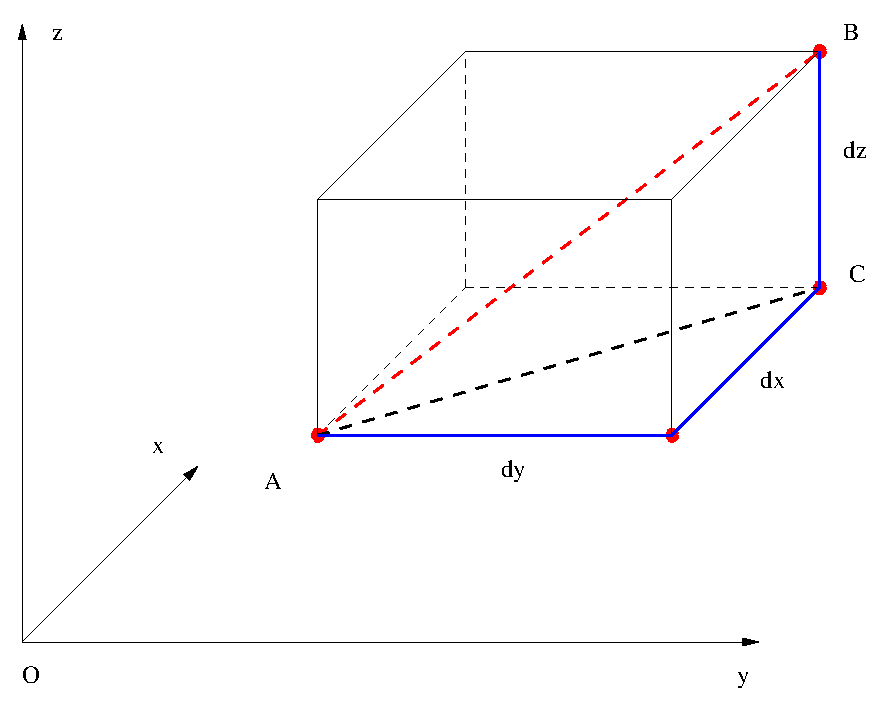
\includegraphics[height=1in]{../../modules/coordinate-systems/pictures/euclidean_distance.eps}
%
%
Example: $P(3,1,2)$ and $Q(1,2,3)$:\pause
%
$$D(P,Q) = \sqrt{(1-3)^2+(2-1)^2+(3-2)^2} = \sqrt{6}\; .$$

\end{frame}
\begin{frame}
 \frametitle{Change of Coordinates}

  Change in original position and orientation $\to$ new coordinates

\pause

Example:
  \begin{itemize}
   \item Move ahead 1m;
   \item Turn a quarter of a circle to the right.
  \end{itemize}
  
%
\begin{table}[h]
\begin{tabular}{lcr}
  \psfrag{P}{$P(3,1,2)$}
  \psfrag{O}{$O(0,0,0)$}  
  \psfrag{x}{$x=3$} 
  \psfrag{y}{$y=1$} 
  \psfrag{z}{$z=2$}     
  \psfrag{A}{$Ox$}
  \psfrag{L}{$Oy$}
  \psfrag{U}{$Oz$}  
  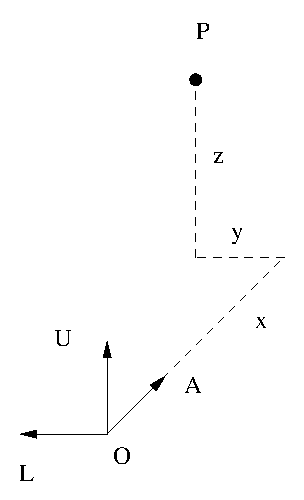
\includegraphics[height=2in]{../../modules/coordinate-systems/pictures/projector.eps}
%
& \hspace{2cm} &
%
\psfrag{P}{$P$}
  \psfrag{Op}{$O'$} 
  \psfrag{O}{$O$}  
  \psfrag{L}{$L$}
  \psfrag{U}{$U$}   
  \psfrag{xp}{$x'=-1$} 
  \psfrag{yp}{$y'=2$} 
  \psfrag{zp}{$z'=2$}     
  \psfrag{Ap}{$A'$}
  \psfrag{Lp}{$L'$}
  \psfrag{Up}{$U'$}  
  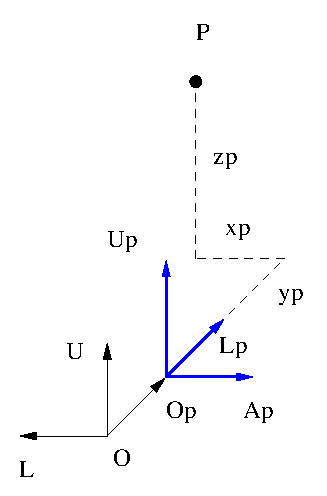
\includegraphics[height=2in]{../../modules/coordinate-systems/pictures/new_frame.eps}
%
\end{tabular}
  \end{table}
%  
%
\pause  
New coordinates of projector: $P \to (x',y',z') = (-1,2,2)$
\end{frame}

\begin{frame}
\frametitle{General formula for this change of coordinates}
%
\begin{table}[h]
\begin{tabular}{lcr}
  \psfrag{P}{$P(x,y,z)$}
  \psfrag{O}{$O(0,0,0)$}  
  \psfrag{x}{$x$} 
  \psfrag{y}{$y$} 
  \psfrag{z}{$z$}     
  \psfrag{A}{$Ox$}
  \psfrag{L}{$Oy$}
  \psfrag{U}{$Oz$}  
  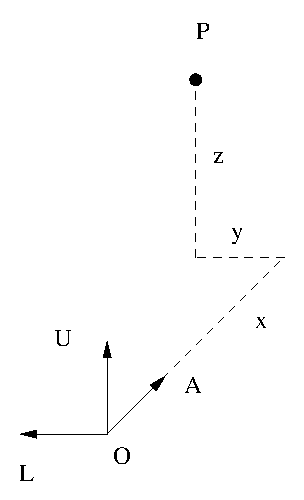
\includegraphics[height=2in]{../../modules/coordinate-systems/pictures/projector.eps}
%
& \hspace{2cm} &
%
\psfrag{P}{$P(x', y', z')$}
  \psfrag{Op}{$O'$} 
  \psfrag{O}{$O$}  
  \psfrag{L}{$L$}
  \psfrag{U}{$U$}   
  \psfrag{xp}{$x'=-y$} 
  \psfrag{yp}{$y'=x-1$} 
  \psfrag{zp}{$z'=z$}     
  \psfrag{Ap}{$A'$}
  \psfrag{Lp}{$L'$}
  \psfrag{Up}{$U'$}  
  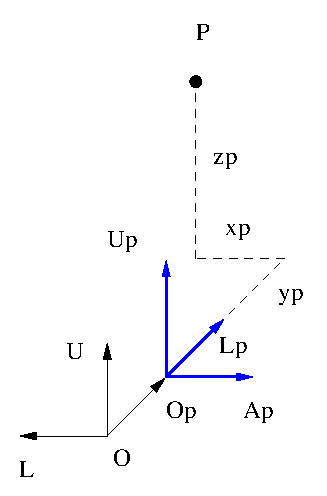
\includegraphics[height=2in]{../../modules/coordinate-systems/pictures/new_frame.eps}
%
\end{tabular}
  \end{table}
%  

\begin{eqnarray*}
 x' = & -y \\
 y' = & x-1 \\
 z' = & z
\end{eqnarray*}
%
Example $Q(x=1,y=2,z=3) \leftrightarrow Q(x'=-2, y'=0,z'=3)$

\end{frame}



\begin{frame}
 \frametitle{Fundamental Philosophy}
  $P(3,1,2)$ and $Q(1,2,3)$ in $(x,y,z)-$coordinates

  $P(-1,2,2)$ and $Q(-2,0,3)$ in $(x',y'z')-$coordinates

  Distance in new coordinates:
 \pause
%
$$d_{x',y',z'}(P,Q) = \sqrt{(-2+1)^2+(0-2)^2+(3-2)^2} = \sqrt{6} = d_{x,y,z}(P,Q)$$

Fundamental Philosophy:\pause
\begin{itemize}
 \item Space doesn't come with coordinates
  \item Natural concepts (such of distance) are independent of coordinates
  \item If a natural concept is defined using coordinates, \\
          the result does not depend on the chosen coordinate system.
\end{itemize}


\end{frame}
\begin{frame}
  \frametitle{Sets in Space}

  $X$ subset of a set $Y$:

  $$X = \{ A \text{ in } Y | A \text{ has property } \mathcal{P} \} \subset Y$$

\pause
Examples  (Fixed point $Q$, fixed $r>0$):

$$X = \{ A \text{ in Space } | d(A,Q) = r \} = S_r(Q)\; ,$$
\pause Sphere of radius $r$ centered at $Q$.\pause

$$B_r(Q) = \{ A \text{ in Space } | d(A,Q) <r \} \; ,$$
\pause  Open ball of radius $r$ centered at $Q$. \pause

$$\overline{B}_r(Q) = \{ A \text{ in Space } | d(A,Q) \leqslant r\} \; ,$$
\pause  Closed ball of radius $r$ centered at $Q$.

\end{frame}
\begin{frame}
 \frametitle{Equation(s) of Subsets}

  $$X = \{ (x,y,z) | x,y,z \text{ satisfy certain relation(s) } \} \; .$$

\pause
Examples:

$\{(x,y,z) | x^2+y^2+z^2 = 1\}$:

\pause
sphere of radius $r=1$ centered at the origin $(0,0,0)$

Also refered to as: sphere $x^2+y^2+z^2 = 1$

\pause
\medskip

$\{ (x,y,z) | x=0 \}$: coordinate Left-Up plane

\pause
\medskip

$\{ (x,y,z) | x=0 \text{ and } y=0 \}$:

intersection of coordinate planes $\rightarrow$ coordinate axis

\pause
\medskip

Can be given by only one equation:

$x^2+y^2 = 0$ $\rightarrow$ $x=0$,$y=0$, and $z$ arbitrary $\rightarrow$

vertical axis above $(0,0)$ in $(x,y)-$plane

\pause
\medskip

Important: Equations in Plane vs. Space.

\end{frame}
\begin{frame}
 \frametitle{Recognizing Spheres from Equations}

  $Q(x_0,y_0,z_0)$, $r>0$, $A(x,y,z)$. Remark: $d(A,Q) = r \longleftrightarrow d^2(A,Q) = r^2$

$$S_r(Q): \quad (x-x_0)^2+(y-y_0)^2+(z-z_0)^2 = r^2$$

\pause
Example:
$$(x-2)^2+(y-0)^2+(z+1)^2=3^2$$
%
$$x^2+y^2+z^2 -4x + 2z -4=0$$

\pause
\begin{itemize}
 \item no mixed terms $xy$, $xz$, or $yz$;
 \item quadratic terms $x^2$, $y^2$, and $z^2$ with the same coefficient.
\end{itemize}

\pause
Examples:
$$x^2+y^2+z^2-4x+2y=0$$
%
\pause
Complete the square:
%
$$(x-2)^2 + (y+1)^2 +z^2 = 5$$
%
Sphere of radius $\sqrt{5}$ centered at $(2,-1,0)$.

\pause
How about $x^2+y^2+z^2 - 4x+2y = -6$? \pause Passes both tests, but ...
%
$$(x-2)^2 + (y+1)^2 +z^2 = -1$$
%
is impossible! No such points, set is empty.

\end{frame}

\section{Polar Coordinates}
% begin module polar-intro
\begin{frame}
\frametitle{Polar Coordinates}
\begin{itemize}
\item  The polar coordinates system is an alternative to the Cartesian coordinates system.
%\item  Instead of specifying horizontal distance and vertical distance, we specify angle and distance from the origin.
\item  Choose a point in the plane called $O$ (the origin).
\item  Draw a ray starting at $O$ called the polar axis.  This ray is usually drawn horizontally to the right.
\end{itemize}
\begin{columns}[c]
\column{.5\textwidth}
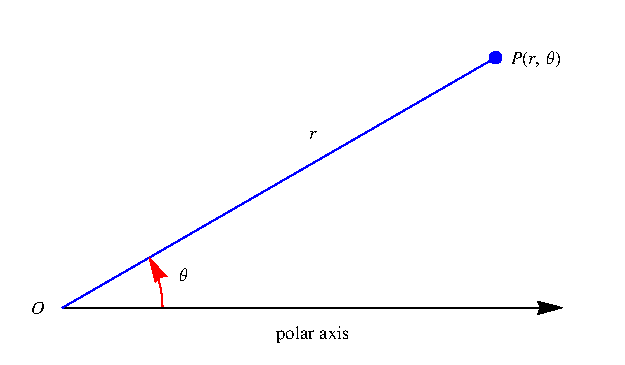
\includegraphics[height=4cm]{polar-curves/pictures/11-03-polar.pdf}%
\column{.5\textwidth}
\begin{itemize}
\item  Let $P$ be a point in the plane.
\item  Let $\theta$ denote the angle between the polar axis and the line $OP$.
\item  Let $r$ denote the length of the line $OP$.
\item  Then $P$ is represented by the ordered pair $(r, \theta )$.
\end{itemize}
\end{columns}
\end{frame}
% end module polar-intro

% begin module polar-questions
\begin{frame}
\begin{enumerate}
\item<1-| alert@2>  What if $\theta$ is negative?
\item<1-| alert@3>  What if $r$ is negative?
\item<1-| alert@4>  What if $r$ is $0$?
\end{enumerate}
\begin{columns}[c]
\column{.5\textwidth}
\uncover<2->{
\psset{xunit=2cm, yunit=2cm}
\begin{pspicture}(-0.9, -1.2)(2,0.2)
\tiny
%force a boudning box:
%\psline[linecolor=red!1](-0.1, -0.1)(-0.21,0.2)
%\psline[linecolor=red!1](1.1, 0.6)(1.1,0.61)
\fcFullDotBlue{0}{0}

%Calculator input: plotCurve{}(1/10 \cos{}t, 1/10 \sin{}t, 0, -3/4 \pi)
\parametricplot[arrows=->, linecolor=\fcColorGraph, plotpoints=100]{0} {-2.35619} {t 57.29578 mul cos 0.3000000 mul t 57.29578 mul sin 0.3000000 mul }
\rput[t] (0,-0.1){$O$}
\rput[l](0.3, -0.2){$\theta=-\frac{3\pi}{4}$}

\psline{->}(0,0)(2,0)
\psline[linecolor=blue](0,0)(-0.707106781, -0.707106781)
\fcFullDotBlue{-0.707106781}{-0.707106781}
\rput[tl](-0.6, -0.7){$\begin{array}{l}(r,\theta)=\left(1, -\frac{3\pi}{4}\right)\\ (x,y)=\left(-\frac{\sqrt{2}}2, -\frac{\sqrt{2}}2 \right) \end{array}$}
\end{pspicture}
}

\uncover<3->{
\psset{xunit=2cm, yunit=2cm}
\begin{pspicture}(-0.9, -1.5)(1.7,0.8)
\tiny
%force a boudning box:
%\psline[linecolor=red!1](-0.1, -0.1)(-0.21,0.2)
%\psline[linecolor=red!1](1.1, 0.6)(1.1,0.61)
\fcFullDotBlue{0}{0}

\parametricplot[arrows=->, linecolor=\fcColorGraph, plotpoints=100]{0} {0.523598776 } {t 57.29578 mul cos 0.3000000 mul t 57.29578 mul sin 0.3000000 mul }
\parametricplot[arrows=->, linecolor=brown, plotpoints=100]{0} {3.665191429 } {t 57.29578 mul cos 0.25 mul t 57.29578 mul sin 0.25 mul }

\rput[t] (0,-0.1){$O$}

\psline{->}(0,0)(1,0)
\psline[linecolor=blue](0,0)(0.866025404, 0.5)
\fcFullDotBlue{0.866025404}{0.5}
\rput[tl](-0.75, -0.5){
$(-r, \theta)$
}
\fcFullDotBlue{-0.866025404}{-0.5}
\psline[linecolor=blue, linestyle=dashed](0,0) (-0.866025404,-0.5)
\rput[tl](0.6, 0.7){$(r, \theta) $}
\end{pspicture}
}
%\ \uncover<2->{%
%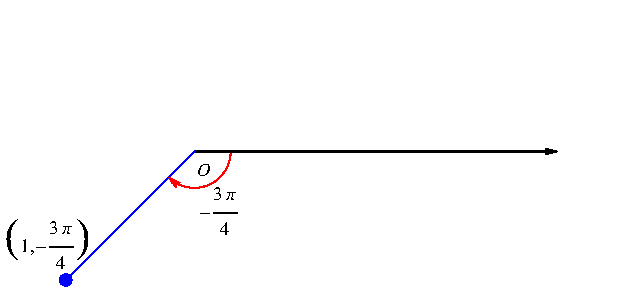
\includegraphics[height=3cm]{polar-curves/pictures/11-03-ex1b.pdf}%
%}%
%\ \uncover<3->{%
%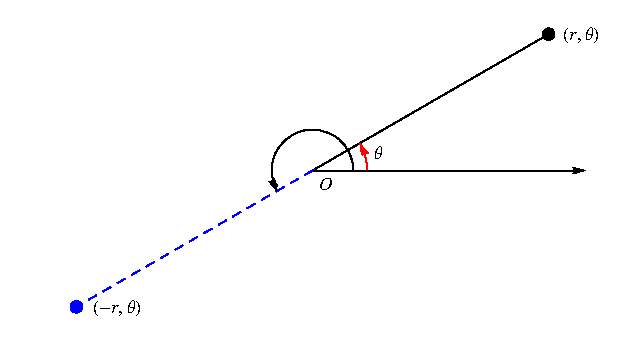
\includegraphics[height=3cm]{polar-curves/pictures/11-03-negativer.pdf}%
%}%
\column{.5\textwidth}
\begin{enumerate}
\item<2-| alert@2>  Positive angles $\theta$ are measured in the counterclockwise direction from $O$.  Negative angles are measured in the clockwise direction.
\item<3-| alert@3>  Points with polar coordinates $(-r, \theta)$ and $(r, \theta)$ lie on the same line through $O$ and at the same distance from $O$, but on opposite sides.
\item<4-| alert@4>  If $r = 0$, then $(r, \theta) = P = O$ for all values of $\theta$.
\end{enumerate}
\end{columns}
\end{frame}
% end module polar-questions

% begin module polar-many-representations
\begin{frame}
\begin{columns}[T]
\column{.5\textwidth}
\uncover<1->{
\psset{xunit=2cm, yunit=2cm}
\begin{pspicture}(-0.9, -1.1)(2,0.5)
\tiny
%force a boudning box:
%\psline[linecolor=red!1](-0.1, -0.1)(-0.21,0.2)
%\psline[linecolor=red!1](1.1, 0.6)(1.1,0.61)
\fcFullDotBlue{0}{0}

%Calculator input: plotCurve{}(1/10 \cos{}t, 1/10 \sin{}t, 0, -3/4 \pi)
\parametricplot[arrows=->, linecolor=\fcColorGraph, plotpoints=100]{0} {3.926990817} {t 57.29578 mul cos 0.3000000 mul t 57.29578 mul sin 0.3000000 mul }
\rput[t] (0,-0.1){$O$}
\rput[l](0.3, 0.3){$\theta=\frac{5\pi}{4}$}

\psline{->}(0,0)(2,0)
\psline[linecolor=blue](0,0)(-0.707106781, -0.707106781)
\fcFullDotBlue{-0.707106781}{-0.707106781}
\rput[tl](-0.6, -0.7){$(r,\theta)=\left(1, \frac{5\pi}{4}\right)$}
\end{pspicture}
}
\uncover<2->{
\psset{xunit=2cm, yunit=2cm}
\begin{pspicture}(-0.9, -1.1)(2,0.5)
\tiny
%force a boudning box:
%\psline[linecolor=red!1](-0.1, -0.1)(-0.21,0.2)
\psline[linecolor=red!1](1.1, 0.5)(1.1,0.51)
\fcFullDotBlue{0}{0}

%Calculator input: plotCurve{}(1/10 \cos{}t, 1/10 \sin{}t, 0, -3/4 \pi)
\parametricplot[arrows=->, linecolor=\fcColorGraph, plotpoints=100]{0} {-2.35619} {t 57.29578 mul cos 0.3000000 mul t 57.29578 mul sin 0.3000000 mul }
\rput[t] (0,-0.1){$O$}
\rput[l](0.3, -0.2){$\theta=-\frac{3\pi}{4}$}

\psline{->}(0,0)(2,0)
\psline[linecolor=blue](0,0)(-0.707106781, -0.707106781)
\fcFullDotBlue{-0.707106781}{-0.707106781}
\rput[tl](-0.6, -0.7){$(r,\theta)=\left(1, -\frac{3\pi}{4}\right)$}
\end{pspicture}
}

%\ \uncover<1->{%
%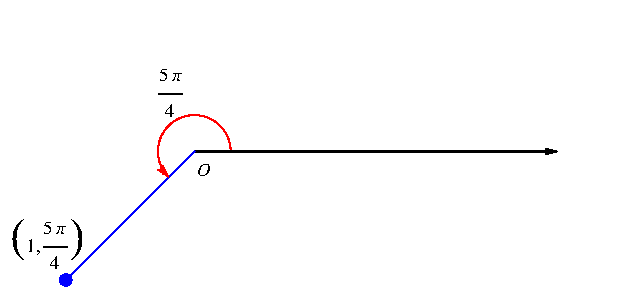
\includegraphics[height=3cm]{polar-curves/pictures/11-03-ex1a.pdf}%
%}%

%\ \uncover<2->{%
%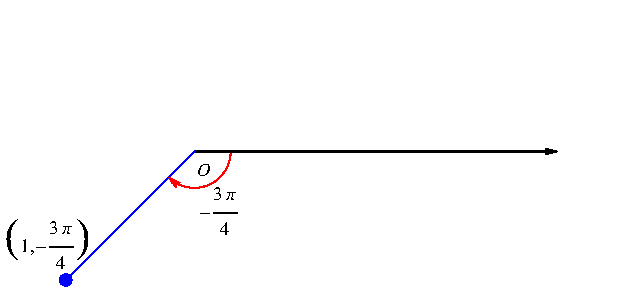
\includegraphics[height=3cm]{polar-curves/pictures/11-03-ex1b.pdf}%
%}%
\column{.5\textwidth}
\uncover<3->{
\psset{xunit=2cm, yunit=2cm}
\begin{pspicture}(-0.9, -1.1)(2,0.5)
\tiny
%force a boudning box:
%\psline[linecolor=red!1](-0.1, -0.1)(-0.21,0.2)
%\psline[linecolor=red!1](1.1, 0.6)(1.1,0.61)
\fcFullDotBlue{0}{0}

%Calculator input: plotCurve{}(1/50 t \cos{}t+3/20 \cos{}t, 1/50 t \sin{}t+3/20 \sin{}t, 0, 13/4 \pi)
\parametricplot[arrows=->, linecolor=\fcColorGraph, plotpoints=400] {0} {10.2102} {t 57.29578 mul cos 0.1500000 mul t 57.29578 mul cos t mul 0.0200000 mul add t 57.29578 mul sin 0.1500000 mul t 57.29578 mul sin t mul 0.0200000 mul add }

\rput[t] (0,-0.1){$O$}
\rput[l](0.3, 0.3){$\theta=\frac{13\pi}{4}$}

\psline{->}(0,0)(2,0)
\psline[linecolor=blue](0,0)(-0.707106781, -0.707106781)
\fcFullDotBlue{-0.707106781}{-0.707106781}
\rput[tl](-0.6, -0.7){$(r,\theta)=\left(1, \frac{13\pi}{4}\right)$}
\end{pspicture}
}

\uncover<4->{
\psset{xunit=2cm, yunit=2cm}
\begin{pspicture}(-0.9, -1.1)(2,0.5)
\tiny
%force a boudning box:
%\psline[linecolor=red!1](-0.1, -0.1)(-0.21,0.2)
\psline[linecolor=red!1](1.1, 0.5)(1.1,0.51)
\fcFullDotBlue{0}{0}

%Calculator input: plotCurve{}(1/10 \cos{}t, 1/10 \sin{}t, 0, -3/4 \pi)
\parametricplot[arrows=->, linecolor=\fcColorGraph, plotpoints=100]{0} {0.785398163} {t 57.29578 mul cos 0.3000000 mul t 57.29578 mul sin 0.3000000 mul }
\rput[t] (0,-0.1){$O$}
\rput[l](0.35, 0.15){$\theta=\frac{\pi}{4}$}

\psline{->}(0,0)(2,0)
\psline[linecolor=blue](0,0)(-0.707106781, -0.707106781)
\fcFullDotBlue{-0.707106781}{-0.707106781}
\psline[linestyle=dashed](0,0)(0.707106781, 0.707106781)
\fcFullDotBlack{0.707106781}{0.707106781}
\rput[tl](-0.6, -0.7){$(r,\theta)=\left(-1, \frac{\pi}{4}\right)$}
\end{pspicture}
}
%\ \uncover<3->{%
%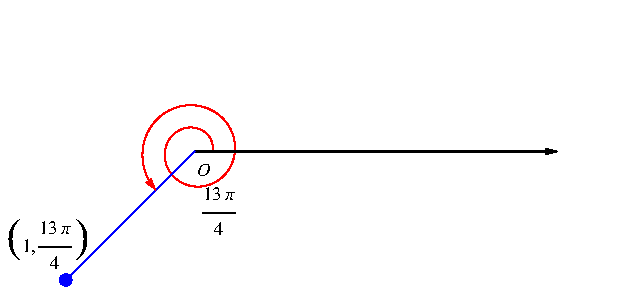
\includegraphics[height=3cm]{polar-curves/pictures/11-03-ex1c.pdf}%
%}%

%\ \uncover<4->{%
%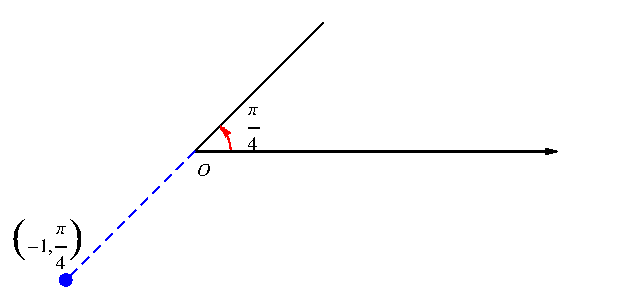
\includegraphics[height=3cm]{polar-curves/pictures/11-03-ex1d.pdf}%
%}%
\end{columns}
\begin{itemize}
\item  There are many ways to represent the same point.
\item<2-| alert@2>  We could use a negative $\theta$.
\item<3-| alert@3>  We could go around more than once.
\item<4-| alert@4>  We could use a negative $r$.
\end{itemize}
\end{frame}
% end module polar-many-representations

%begin module polar-two-points-coincide-iff
\begin{frame}
\begin{itemize}
\item Let $P_1$ be point  with polar coordinates $(r_1, \theta_1)$.
\item Let $P_2$ be point  with polar coordinates $(r_2, \theta_2)$.
\end{itemize}

\uncover<2->{
\begin{observation}
$P_1$ coincides with $P_2$ if one of the three mutually exclusive possibilities holds:
\begin{itemize}
\item<alert@3> $r_1=r_2\neq 0$ and $\theta_2=\theta_1+2k\pi, k\in \mathbb Z $,
\item<alert@4> $r_1=-r_2\neq 0$ and $\theta_2=\theta_1+(2k+1)\pi, k\in \mathbb Z$,
\item $r_1=r_2=0 $ and $\theta$ is arbitrary.
\end{itemize}
\end{observation}
}
\begin{columns}
\column{.5\textwidth}
\only<3>{
\psset{xunit=2cm, yunit=2cm}
\begin{pspicture}(-0.9, -1.1)(2,0.75) 
\tiny 
%force a boudning box:
%\psline[linecolor=red!1](-0.1, -0.1)(-0.21,0.2)
%\psline[linecolor=red!1](1.1, 0.6)(1.1,0.61)
\psFullDotBlue{0}{0}

%Calculator input: plotCurve{}(1/10 \cos{}t, 1/10 \sin{}t, 0, -3/4 \pi)
\parametricplot[arrows=->, linecolor=\psColorGraph, plotpoints=100]{0} {3.926990817} {t 57.29578 mul cos 0.3000000 mul t 57.29578 mul sin 0.3000000 mul }
\rput[t] (0,-0.1){$O$}
\rput[l](0.3, 0.3){$\theta_1$}

\psline{->}(0,0)(2,0)
\psline[linecolor=blue](0,0)(-0.707106781, -0.707106781)
\psFullDotBlue{-0.707106781}{-0.707106781}
\rput[tl](-0.6, -0.7){$(r_1,\theta_1)$}
\end{pspicture} 
}
\uncover<4>{
\psset{xunit=2cm, yunit=2cm}
\begin{pspicture}(-0.9, -1.1)(2,0.75) 
\tiny 
%force a boudning box:
%\psline[linecolor=red!1](-0.1, -0.1)(-0.21,0.2)
\psline[linecolor=red!1](1.1, 0.5)(1.1,0.51)
\psFullDotBlue{0}{0}

%Calculator input: plotCurve{}(1/10 \cos{}t, 1/10 \sin{}t, 0, -3/4 \pi)
\parametricplot[arrows=->, linecolor=\psColorGraph, plotpoints=100]{0} {-2.35619} {t 57.29578 mul cos 0.3000000 mul t 57.29578 mul sin 0.3000000 mul }
\rput[t] (0,-0.1){$O$}
\rput[l](0.3, -0.2){$\theta_1$}

\psline{->}(0,0)(2,0)
\psline[linecolor=blue](0,0)(-0.707106781, -0.707106781)
\psFullDotBlue{-0.707106781}{-0.707106781}
\rput[tl](-0.6, -0.7){$(r_1,\theta_1)$}
\end{pspicture} 
}

%\ \uncover<1->{%
%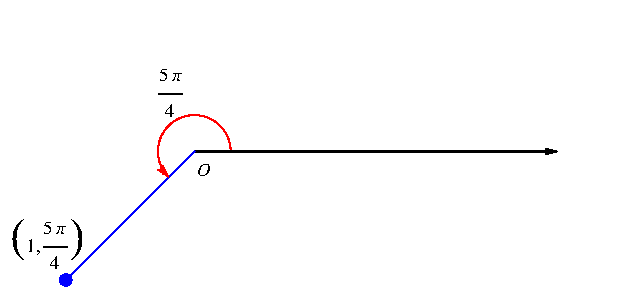
\includegraphics[height=3cm]{polar-curves/pictures/11-03-ex1a.pdf}%
%}%

%\ \uncover<2->{%
%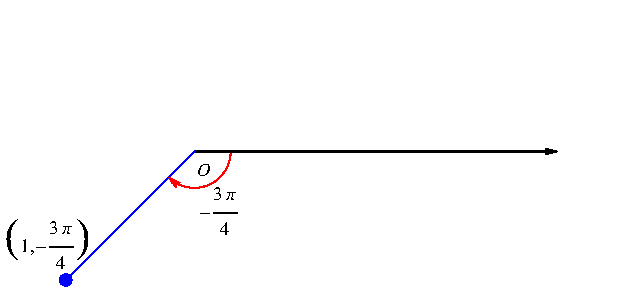
\includegraphics[height=3cm]{polar-curves/pictures/11-03-ex1b.pdf}%
%}%

\vspace{2cm}
\column{.5\textwidth}
\only<3>{
\psset{xunit=2cm, yunit=2cm}
\begin{pspicture}(-0.9, -1.1)(2,0.75) 
\tiny 
%force a boudning box:
%\psline[linecolor=red!1](-0.1, -0.1)(-0.21,0.2)
%\psline[linecolor=red!1](1.1, 0.6)(1.1,0.61)
\psFullDotBlue{0}{0}

%Calculator input: plotCurve{}(1/50 t \cos{}t+3/20 \cos{}t, 1/50 t \sin{}t+3/20 \sin{}t, 0, 13/4 \pi)
\parametricplot[arrows=->, linecolor=\psColorGraph, plotpoints=400] {0} {10.2102} {t 57.29578 mul cos 0.1500000 mul t 57.29578 mul cos t mul 0.0200000 mul add t 57.29578 mul sin 0.1500000 mul t 57.29578 mul sin t mul 0.0200000 mul add }

\rput[t] (0,-0.1){$O$}
\rput[l](0.3, 0.3){$\theta_2=\theta_1+2\pi$}

\psline{->}(0,0)(2,0)
\psline[linecolor=blue](0,0)(-0.707106781, -0.707106781)
\psFullDotBlue{-0.707106781}{-0.707106781}
\rput[tl](-0.6, -0.7){$(r_2, \theta_2)=(r_1,\theta_1+2\pi)$}
\end{pspicture} 
}

\uncover<4>{
\psset{xunit=2cm, yunit=2cm}
\begin{pspicture}(-0.9, -1.1)(2,0.75) 
\tiny 
%force a boudning box:
%\psline[linecolor=red!1](-0.1, -0.1)(-0.21,0.2)
\psline[linecolor=red!1](1.1, 0.5)(1.1,0.51)
\psFullDotBlue{0}{0}

%Calculator input: plotCurve{}(1/10 \cos{}t, 1/10 \sin{}t, 0, -3/4 \pi)
\parametricplot[arrows=->, linecolor=\psColorGraph, plotpoints=100]{0} {0.785398163} {t 57.29578 mul cos 0.3000000 mul t 57.29578 mul sin 0.3000000 mul }
\rput[t] (0,-0.1){$O$}
\rput[l](0.35, 0.15){$\theta_2=\theta_1+\pi$}

\psline{->}(0,0)(2,0)
\psline[linecolor=blue](0,0)(-0.707106781, -0.707106781)
\psFullDotBlue{-0.707106781}{-0.707106781}
\psline[linestyle=dashed](0,0)(0.707106781, 0.707106781)
\psFullDotBlack{0.707106781}{0.707106781}
\rput[tl](-0.6, -0.7){$(r_2, \theta_2)=(-r_1,\theta_1+\pi)$}
\end{pspicture} 
}
%\ \uncover<3->{%
%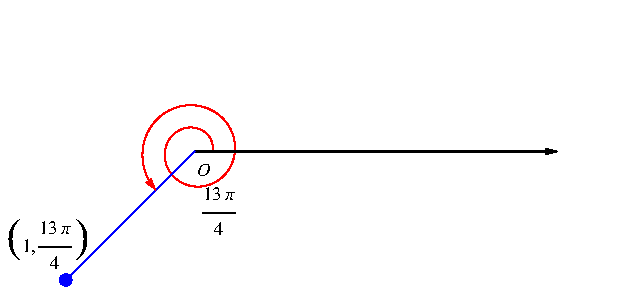
\includegraphics[height=3cm]{polar-curves/pictures/11-03-ex1c.pdf}%
%}%

%\ \uncover<4->{%
%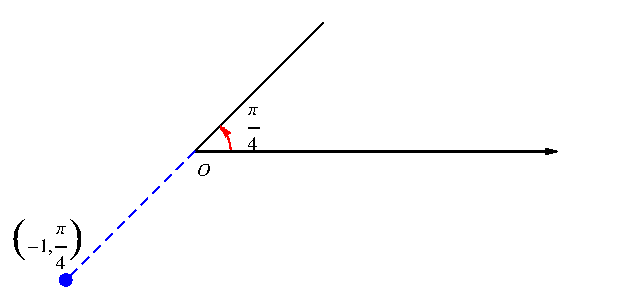
\includegraphics[height=3cm]{polar-curves/pictures/11-03-ex1d.pdf}%
%}%

\vspace{2cm}
\end{columns}
\end{frame}
%end module polar-two-points-coincide-iff
% begin module polar-to-cartesian
\begin{frame}
\begin{itemize}
\item  How do we go from polar coordinates to Cartesian coordinates?
\item<2->  Suppose a point has polar coordinates $(r, \theta )$ and Cartesian coordinates $(x,y)$.
\item<8->  How do we go from Cartesian coordinates to polar coordinates?
\end{itemize}
\begin{columns}[c]
\column{0.5\textwidth}
\psset{xunit=4cm, yunit=4cm}
\begin{pspicture}(-0.2, -0.2)(1.400000,0.9)
\tiny
%force a boudning box:
\psline[linecolor=red!1](-0.1, -0.1)(-0.21,0.2)
\psline[linecolor=red!1](1.1, 0.6)(1.1,0.61)
\psaxes[arrows=<->, ticks=none, labels=none](0,0)(-0.2, -0.2)(1, 0.8)
\rput(-0.03, 0.8){$y$}
\rput(1,-0.03){$x$}
%\fcAxesStandard{-0.2}{-0.2}{1}{0.8}

%Calculator input: plotCurve{}(1/5 \cos{}t, 1/5 \sin{}t, 0, 1/6 \pi)
\parametricplot[arrows=->, linecolor=red, plotpoints=1000] {0}{0.523599}{t 57.29578 mul cos 0.2 mul t 57.29578 mul sin 0.2 mul }
\psline[linecolor=blue](0,0)(0.866025404, 0.5)
\rput(0.22, 0.06){$\theta$}

\fcFullDotBlue{0.866025404}{0.5}
\psline(0.866025404,0.5)(0.866025404,0)
\psline(0.846025404, 0)(0.846025404, 0.02)(0.866025404, 0.02)
\rput[l](0.9, 0.5){$P(r,\theta) =(x,y)$}

\uncover<6>{
\psline{<-}(0.89, 0)(0.89, 0.2)
}
\uncover<6->{
\rput(0.89,0.25){$\alert<6,10>{y}$}
}
\uncover<6>{
\psline{->}(0.89, 0.3)(0.89, 0.5)
}
\uncover<4>{
\psline{<-}(0, -0.02)(0.385, -0.02)
}
\uncover<4->{
\rput(0.435,-0.02){$\alert<4,10>{x}$}
}
\uncover<4>{
\psline{->}(0.485, -0.02)(0.866025404, -0.02)
}
\rput[tr](-0.03, -0.03){$O$}
\rput(0.4, 0.3){$\alert<4,6,9,10>{r}$}
\end{pspicture}
%\ \uncover<2->{%
%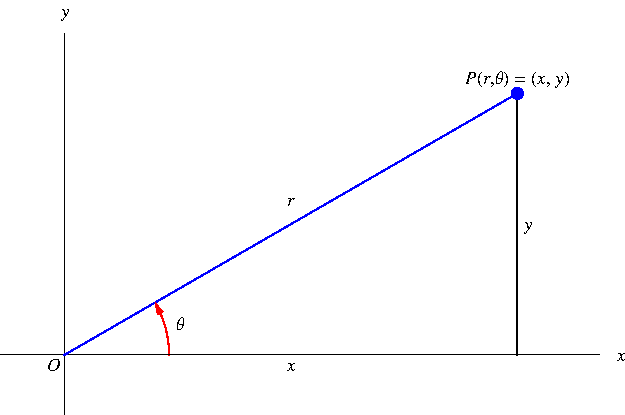
\includegraphics[height=5cm]{polar-curves/pictures/11-03-conversion.pdf}%
%}%
\column{.5\textwidth}
$
\renewcommand{\arraystretch}{1.5}
\begin{array}{rcl}
\alert<7>{x} &\alert<7>{=}&\uncover<7->{\alert<7>{r\cos \theta} } \\
\alert<7>{y}&\alert<7>{=}& \uncover<7->{\alert<7>{r\sin \theta}} \\\hline
\uncover<3->{\alert<3,4,7>{\cos\theta}} & \uncover<3->{\alert<3,4,7>{=}} &\displaystyle \uncover<4->{\alert<4,7>{\frac{x}{r} }} \\
\uncover<3->{\alert<5,6,7>{\sin \theta}} &\uncover<3->{ \alert<5,6,7>{= }} & \displaystyle \uncover<6->{\alert<6,7>{\frac{y}{r}}}\\
\uncover<9->{\alert<handout:0| 9-10>{r^2} &\alert<9,10>{=}& \uncover<10->{\alert<10>{x^2 + y^2}}}\\\hline
\alert<8,9,10,11>{ r}&\alert<8,9,10,11>{=}&\uncover<11->{\alert<11>{ \sqrt{x^2+y^2}}} \\
\alert<12,13>{\theta} &\alert<12,13>{=}&  
\uncover<13->{\alert<13>{\arcsin \left(\frac{y}{r}\right)  \text{\quad if } x>0}}\\ 
\uncover<13->{
&\alert<13>{=}&\alert<13>{\arccos \left(\frac{x}{r}\right)  \text{\quad if } y>0}}\\
\uncover<13->{&\alert<13>{=}&\alert<13>{\arctan \left(\frac{y}{x}\right)  \text{\quad if } x>0}}
\end{array}
$


\end{columns}
\end{frame}
% end module polar-to-cartesian

% begin module polar-to-cartesian-ex2
\begin{frame}
\begin{example} 
Convert the point $(\alert<handout:0| 4>{2}, \alert<handout:0| 6>{\frac{\pi}{3}})$ from polar to Cartesian coordinates.
\[
\uncover<2->{%
x = \alert<handout:0| 3-4>{r}\cos \alert<handout:0| 5-6>{\theta} = %
}%
\uncover<3->{%
\alert<handout:0| 3-4>{\uncover<4->{2}}\alert<handout:0| 7-8>{ \cos } \alert<handout:0| 5-8>{\uncover<6->{\frac{\pi}{3}}} %
}%
\uncover<7->{%
= 2\left( \alert<handout:0| 7-8>{\uncover<8->{\frac{ 1}{ 2 } } } \right) \uncover<9->{ = 1}%
}%
\]
\[
\uncover<2->{%
y = r\sin \theta = %
}%
\uncover<10->{%
2\alert<handout:0| 11-12>{\sin \frac{\pi}{3}}%
}%
\uncover<11->{%
= 2\left( \alert<handout:0| 11-12>{ \uncover<12->{ \frac{ \sqrt{ 3 }}{2}}}\right) \uncover<13->{ = \sqrt{3}}%
}%
\]
\uncover<14->{%
Therefore the point with polar coordinates $(2,\frac{\pi}{3})$ has Cartesian coordinates $(1,\sqrt{3})$.
}%
\end{example}
\end{frame}
% end module polar-to-cartesian-ex2

% begin module polar-to-cartesian-ex3
\begin{frame}
\begin{example}
\begin{columns}
\column{0.25\textwidth}
\psset{xunit=0.65cm, yunit=0.65cm}
\begin{pspicture}(-1,-1)(2,2)
\tiny
\fcAxesStandard{-1.5}{-1.5}{1.5}{1.5}
\fcLabels{1.5}{1.5}
\uncover<9->{%
\fcFullDot{1}{-1}%
}%
\uncover<11->{% 
\fcAngleDegrees[arrows=->, linecolor=red]{0}{315}{0.2} { }%
\rput[b](-0.3, 0.2){$\frac{7\pi}{4}$}
\psline(0,0)(1,-1)
}%
\uncover<13->{%
\fcAngleDegrees{0}{-45}{0.4}{}
\rput[t](0.6, -0.2){$-\frac{\pi}{4}$}
}%
\end{pspicture}
\column{0.75\textwidth}
Represent the point with Cartesian coordinates $(1,-1)$ in terms of polar coordinates.
\end{columns}
\begin{columns}
\column{.6\textwidth}
\begin{itemize}
\item<3-| alert@3-4>  Suppose $r$ is positive.
\item<7->  $\tan \theta = -1$ for $\theta = \alert<handout:0| 10>{\frac{3\pi}{4}}, \alert<handout:0| 10-11>{\frac{7\pi}{4}}$, and many other angles.
\item<8-| alert@8-9>  $(1,-1)$ is in the \uncover<9->{fourth} quadrant.
\item<10->  Of the two values above, only \alert<handout:0| 10-11>{$\theta = \uncover<11->{\frac{7\pi}{4}}$} gives a point in the fourth quadrant.
\item<12->  Therefore one possible representation of $(1,-1)$ in polar coordinates is $(\sqrt{2}, 7\pi/4)$.
\item<13->  $(\sqrt{2}, -\pi /4)$ is another.
\end{itemize}
\column{.4\textwidth}
\begin{eqnarray*}
\uncover<2->{%
r%
}%
& \uncover<2->{ = } &%
\uncover<2->{%
\uncover<-3>{\alert<handout:0| 3>{\pm}} \sqrt{x^2+y^2}%
}\\%
& \uncover<5->{ = } &%
\uncover<5->{%
\sqrt{1^2 + (-1)^2}%
}\\% = \sqrt{2}%
& \uncover<5->{ = } &%
\uncover<5->{%
\sqrt{2}%
}\\% = \sqrt{2}%
&&\\
\uncover<2->{%
\tan \theta%
}%
& \uncover<2->{ = } &%
\uncover<2->{%
\frac{y}{x}%
}\\%
& \uncover<6->{ = } &%
\uncover<6->{%
-1%
}\\%
\end{eqnarray*}
\end{columns}
\end{example}
\end{frame}
% end module polar-to-cartesian-ex3

% begin module polar-intersection-ex3
\begin{frame}
\begin{example} %[Example 3, p. 688]
Find all points of intersection of the polar curves $r = \frac{1}{2}$ and $r = \cos (2\theta)$.
\begin{columns}[c]
\column{.4\textwidth}

\psset{xunit=1.8cm, yunit=1.8cm}
\begin{pspicture}(-1.5, -1.5)(1.5,1.5)
\tiny
\fcAxesStandard{-1.4}{-1.4}{1.4}{1.4}
%Calculator command: drawPolar{}(1/2, 0, 2 \pi)
\parametricplot[linecolor=\fcColorGraph, plotpoints=1000, algebraic=false]{0}{6.28319}{ 0.5 t 57.29578 mul cos mul 0.5 t 57.29578 mul sin mul }
%Calculator command: drawPolar{}(\cos{}(2 t), 0, 2 \pi)
\parametricplot[linecolor=\fcColorGraph, plotpoints=1000, algebraic=false]{0}{6.28319}{t 2 mul 57.29578 mul cos t 57.29578 mul cos mul t 2 mul 57.29578 mul cos t 57.29578 mul sin mul }

\rput[tr](-0.8, -0.8){$r=\frac{1}{2}$}
\psline{->}(-0.75, -0.75)(-0.353553391, -0.353553391)
\rput[lt] (0.2, -1){$r=\cos (2\theta)$}

\uncover<4->{
\fcFullDotBlack{0.433013}{0.25}
\fcFullDotBlack{-0.433013}{0.25}
\fcFullDotBlack{-0.433013}{-0.25}
\fcFullDotBlack{0.433013}{-0.25}
}
\uncover<6->{
\fcFullDotBlack{0.25}{0.433013}
\fcFullDotBlack{0.25}{-0.433013}
\fcFullDotBlack{-0.25}{-0.433013}
\fcFullDotBlack{-0.25}{0.433013}
}
\uncover<9>{
\pscircle*[linecolor=red](0.433013,0.25){0.09}
\pscircle*[linecolor=red](-0.433013,0.25){0.09}
\pscircle*[linecolor=red](-0.433013,-0.25){0.09}
\pscircle*[linecolor=red](0.433013,-0.25){0.09}
}
\uncover<10>{
\pscircle*[linecolor=red](0.25,0.433013){0.09}
\pscircle*[linecolor=red](0.25,-0.433013){0.09}
\pscircle*[linecolor=red](-0.25,-0.433013){0.09}
\pscircle*[linecolor=red](-0.25,0.433013){0.09}
}
\end{pspicture}

%\ \only<handout:0| -3>{%
%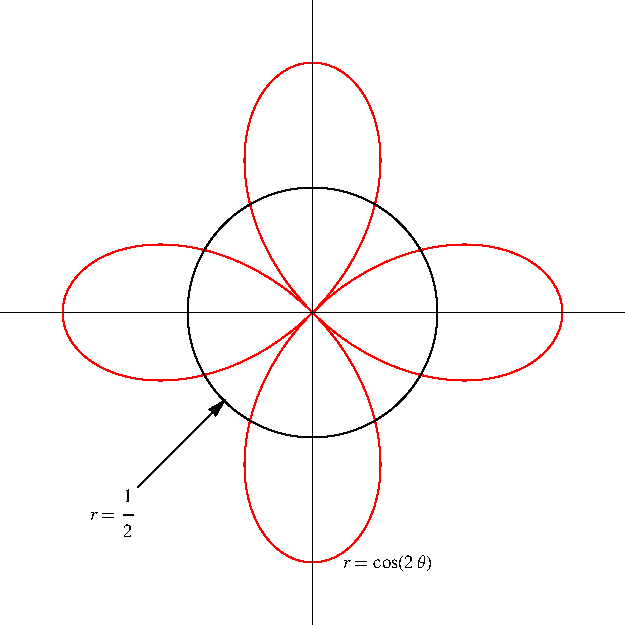
\includegraphics[height=5cm]{polar-curves/pictures/11-04-ex3a.pdf}%
%}%
%\only<handout:0| 4-5>{%
%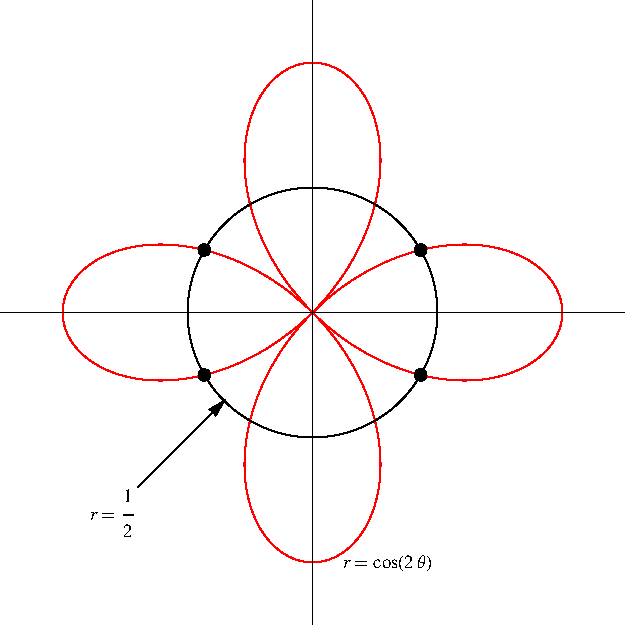
\includegraphics[height=5cm]{polar-curves/pictures/11-04-ex3b.pdf}%
%}%
%\only<6-8>{%
%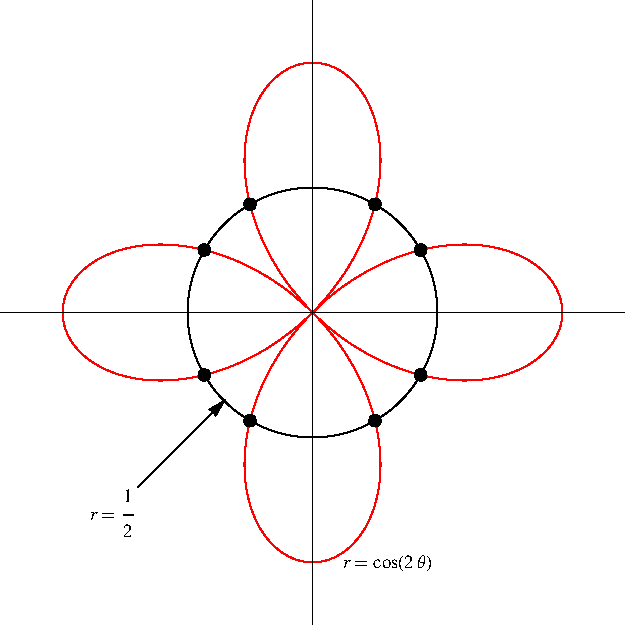
\includegraphics[height=5cm]{polar-curves/pictures/11-04-ex3c.pdf}%
%}%
%\only<handout:0| 9>{%
%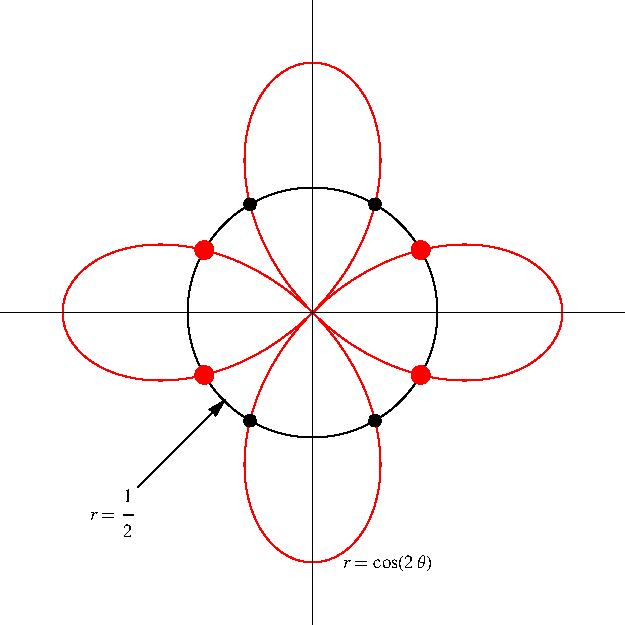
\includegraphics[height=5cm]{polar-curves/pictures/11-04-ex3d.pdf}%
%}%
%\only<handout:0| 10->{%
%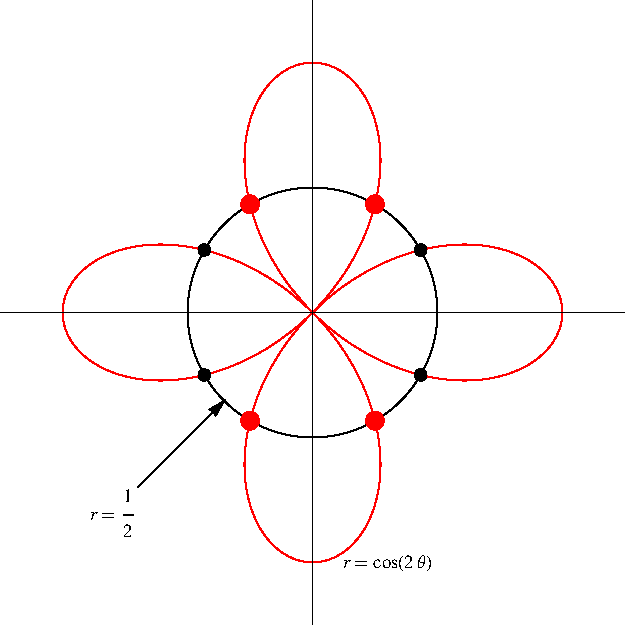
\includegraphics[height=5cm]{polar-curves/pictures/11-04-ex3e.pdf}%
%}%
\column{.6\textwidth}
\abovedisplayskip=0pt
\belowdisplayskip=0pt
\begin{eqnarray*}
\uncover<2->{%
\cos 2\theta%
}%
& \uncover<2->{ = } &%
\uncover<2->{%
\frac{1}{2}%
}\\%
\uncover<3->{%
2\theta%
}%
& \uncover<3->{ = } &%
\uncover<3->{%
\frac{\pi}{3}, \frac{5\pi}{3}, \frac{7\pi}{3}, \frac{11\pi}{3}%
}\\%
\uncover<4->{%
\theta%
}%
& \uncover<4->{ = } &%
\uncover<4->{%
\frac{\pi}{6}, \frac{5\pi}{6}, \frac{7\pi}{6}, \frac{11\pi}{6}%
}%
\end{eqnarray*}
\begin{itemize}
\item<5->  This only gives four points.
\item<6->  There are actually eight.
\item<7->  The circle $r = \frac{1}{2}$ also has polar equation $r = -\frac{1}{2}$.
\item<8->  To find all eight points, solve \alertNoH{ 9}{$\cos (2\theta )= \frac{1}{2}$} and \alertNoH{ 10}{$\cos (2\theta) = -\frac{1}{2}$}.
\end{itemize}
\end{columns}
\end{example}
\end{frame}
% end module polar-intersection-ex3


\section{Cylindrical Coordinates}
\begin{frame}
 \frametitle{Cylindrical coordinates}
\begin{columns}
\column{0.4\textwidth}
%
  \psfrag{P}{$P$}
  \psfrag{O}{$O$}  
  \psfrag{xp}{$x_P$} 
  \psfrag{yp}{$y_P$} 
  \psfrag{zp}{$z_P$}     
  \psfrag{rp}{$r_P$}
  \psfrag{thp}{$\theta_P$}
  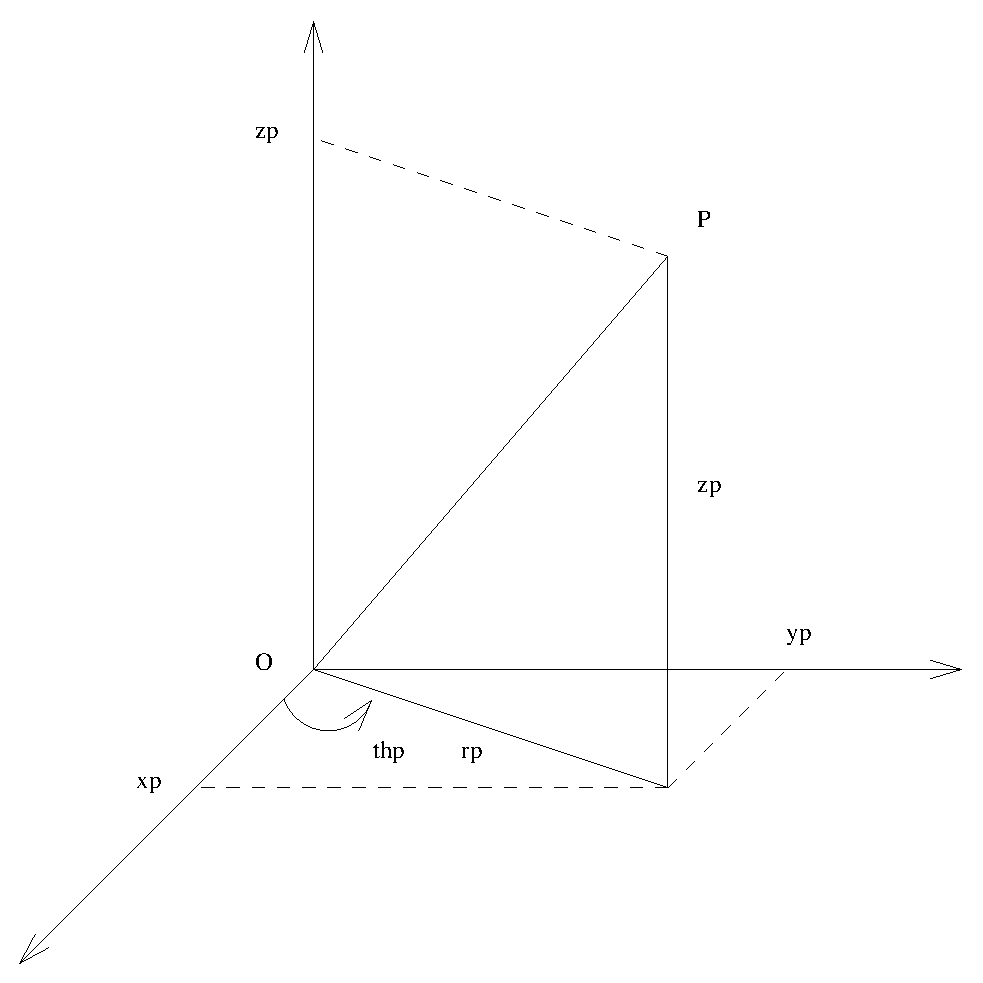
\includegraphics[height=2in]{../../modules/coordinate-systems/pictures/cylindrical_coordinates.eps}
  %\caption{Cylindrical coordinates}
  %\label{fig:cylindrical-coordinates}
%
\column{0.6\textwidth}
$$P(x,y,z) \Longleftrightarrow P(r, \theta, z)$$

\begin{itemize}
    \item Polar in $Oxy$ -- $(r, \theta)$;
    \item Rectangular in $Orz$ -- $(r, z)$.
\end{itemize}
\end{columns}

\end{frame}

\begin{frame}

\begin{columns}
\column{0.4\textwidth}
  \psfrag{P}{$P$}
  \psfrag{O}{$O$}  
  \psfrag{xp}{$x_P$} 
  \psfrag{yp}{$y_P$} 
  \psfrag{zp}{$z_P$}     
  \psfrag{rp}{$r_P$}
  \psfrag{thp}{$\theta_P$}
  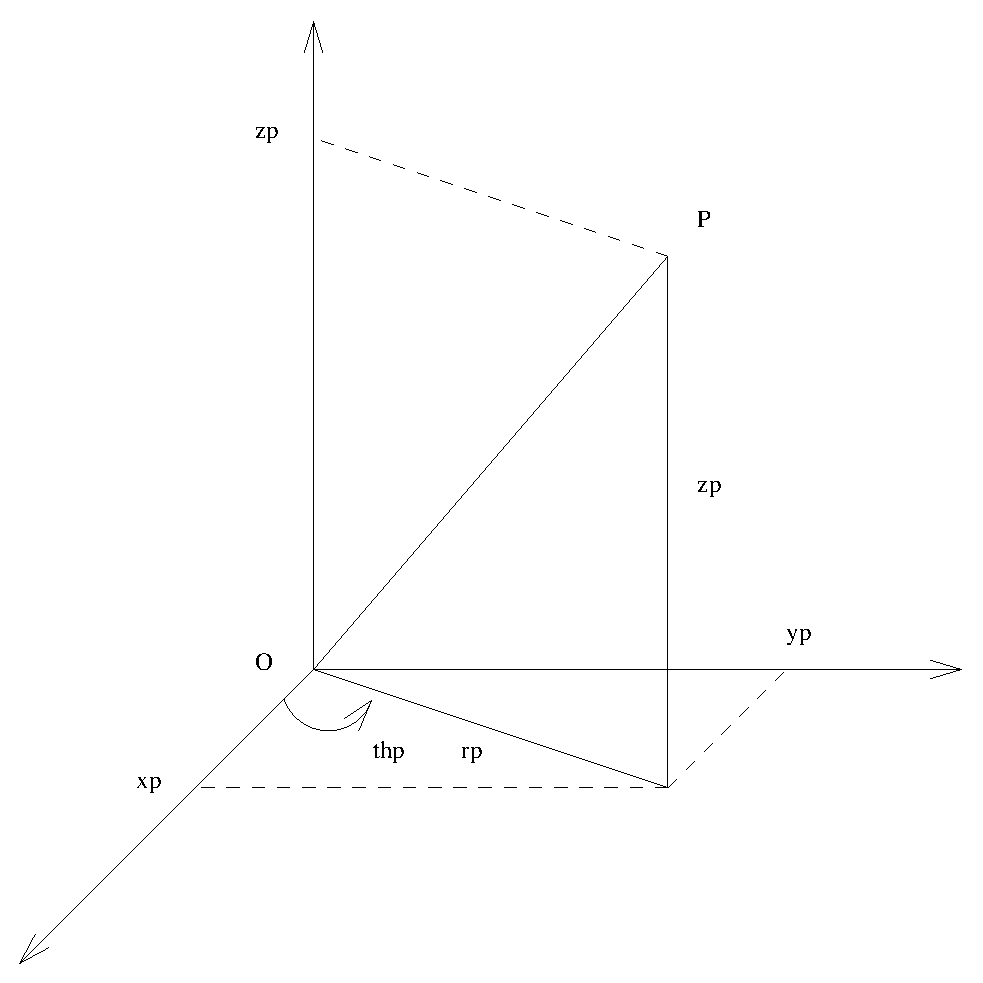
\includegraphics[height=2in]{../../modules/coordinate-systems/pictures/cylindrical_coordinates.eps}
  %\caption{Cylindrical coordinates}
  %\label{fig:cylindrical-coordinates}
%
\column{0.6\textwidth}
To transform cylindrical to rectangular coordinates:\pause
$$x=r\cos\theta \quad , \quad y = r\sin\theta \quad , \quad z_{r} = z_{c}$$

Rectangular to cylindrical:\pause
$$r= \sqrt{x^2+y^2} \quad , \quad z_{c}=z_{r}$$
$$\cos\theta = \frac{x}{r} \quad , \quad \sin\theta = \frac{y}{r}\; .$$
\end{columns}
\end{frame}

\begin{frame}
\frametitle{Constant Coordinate Sets}
\begin{columns}
\column{0.4\textwidth}
  \psfrag{P}{$P$}
  \psfrag{O}{$O$}  
  \psfrag{xp}{$x_P$} 
  \psfrag{yp}{$y_P$} 
  \psfrag{zp}{$z_P$}     
  \psfrag{rp}{$r_P$}
  \psfrag{thp}{$\theta_P$}
  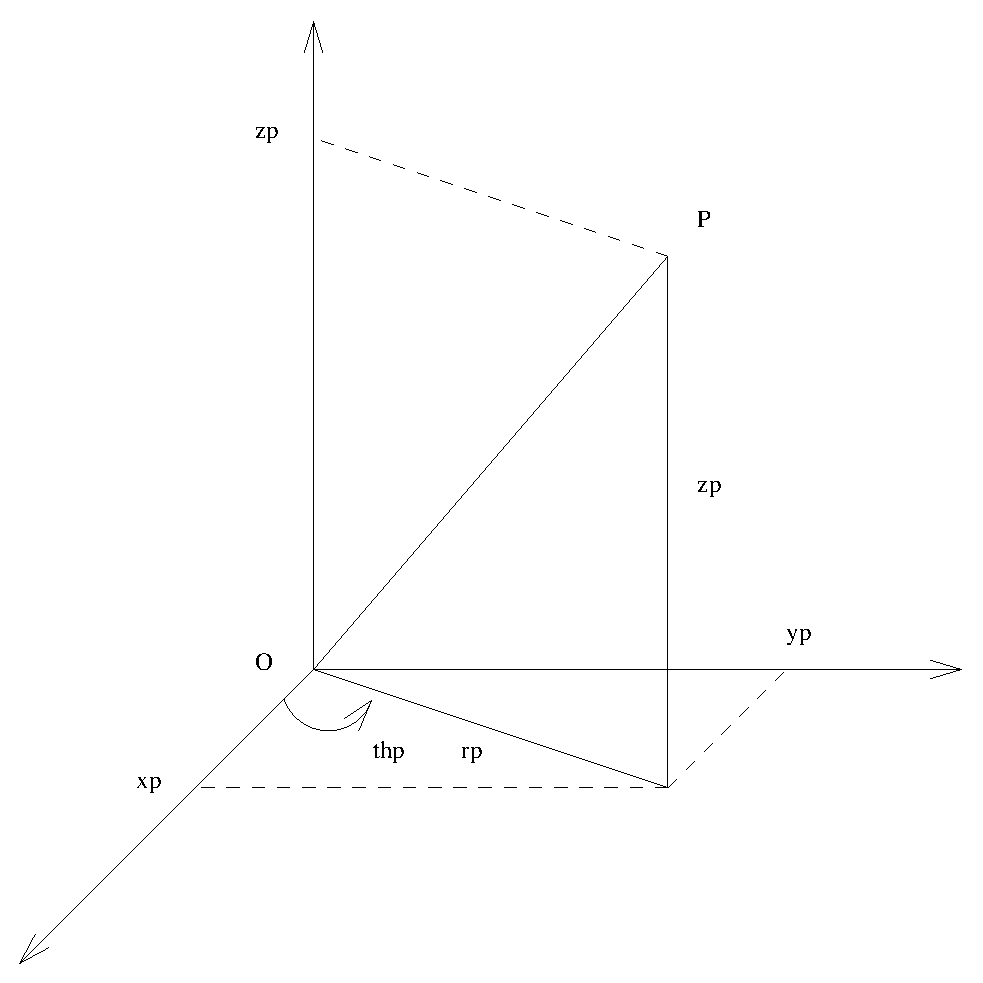
\includegraphics[height=2in]{../../modules/coordinate-systems/pictures/cylindrical_coordinates.eps}
\column{0.6\textwidth}

Surfaces:
\begin{itemize}
  \item $r$ constant \pause$\to$ vertical cylinder;
  \item $\theta$ constant \pause$\to$ vertical half plane;
  \item $z$ constant \pause$\to$ horizontal plane.\pause
\end{itemize}
%
Curves:
\begin{itemize}
 \item $\theta, z$ constant \pause$\to$ horizontal ray;
\item $r, z$ constant \pause$\to$ horizontal circle;
\item $r, \theta$ constant \pause$\to$ vertical line.
\end{itemize}
\end{columns}
\end{frame}
\section{Spherical Coordinates}
\begin{frame}
 \frametitle{Spherical Coordinates}
\begin{columns}
\column{0.55\textwidth}
%  \psfrag{P}{$P$}
%  \psfrag{O}{$O$}
%  \psfrag{xp}{$x_P$}
%  \psfrag{yp}{$y_P$}
%  \psfrag{zp}{$z_P$}
%  \psfrag{rho}{$\rho_P$}
%  \psfrag{thp}{$\theta_P$}
%  \psfrag{phi}{$\phi_P$}
\psset{xunit=1cm, yunit=1cm}
\begin{pspicture}(-2.1,-2.5)(5,5.2)
\tiny
\renewcommand{\fcScreen}{[-1 -0.4 -0.25] -1}
\fcBoundingBox{-2.1}{-2.5}{2}{2}
\fcAxesIIId{5}{5}{5}
\fcPutIIId[r]{[0 -0.15 0.15]}{$O$}
\fcLineIIId[linestyle=dotted]{[3 0 0]}{[3 3 0]}
\fcLineIIId[linestyle=dotted]{[3 3 0]}{[0 3 0]}
\fcLineIIId[linestyle=dotted]{[0 0 0]}{[0 3 0]}
\fcLineIIId{[0 0 0]}{[3 3 0]}
\fcLineIIId{[3 3 0]}{[3 3 3]}
\fcLineIIId{[0 0 3]}{[3 3 3]}
\fcPutIIId[l]{[3.1 3.1 3.1]}{$P$}
\fcPutIIId[r]{[1.5 -0.1 0]}{$x_P$}
\fcPutIIId[t]{[3 3 0]}{$Q$}
\fcPutIIId[b]{[0 1.5 0]}{$y_P$}
\fcPutIIId[l]{[3 3 1.5]}{$~~z_P$}
\fcPutIIId[r]{[0 0 1.5]}{$z_P~~$}
\uncover<2->{%
\fcLineIIId{[0 0 0]}{[3 3 3]}
\uncover<3>{\fcLineIIId[linecolor=red, linewidth=2pt]{[0 0 0]}{[3 3 3]}}%
\fcPutIIId[r]{[2.1 2.1 2.1]}{$\rho_P$}
\fcPutIIId[rt]{[1 1 1.5]}{$\phi_P~~$}
\fcPutIIId[tr]{[1.8 0.9 0]}{$\theta_P$}%
\fcAngleIIId[linecolor=red, arrows=->]{[0 0 1]}{[3 3 3]}{1.7}%
\uncover<4>{\fcAngleIIId[linecolor=red, linewidth=2pt, arrows=->]{[0 0 1]}{[3 3 3]}{1.7}}%
\fcAngleIIId[linecolor=red, arrows=->]{[1 0 0]}{[3 3 0]}{1.7}%
\uncover<5>{\fcAngleIIId[linecolor=red, arrows=->, linewidth=2pt]{[1 0 0]}{[3 3 0]}{1.7}}%
}%
\uncover<8>{\fcLineIIId[arrows=->, linecolor=red, linewidth=2pt]{[0 0 0]}{[5 5 5]}}%
\uncover<10>{%
\fcAngleIIId[linecolor=red, linewidth=2pt]{[0 0 1]}{[1 1 0]}{2}%
\fcAngleIIId[linecolor=red, linewidth=2pt, arrows=->]{[1 1 0]}{[0 0 -1]}{2}%
}%
\uncover<12>{%
\fcAngleIIId[linecolor=red, linewidth=2pt]{[1 0 0]}{[0 1 0]}{2}%
\fcAngleIIId[linecolor=red, linewidth=2pt]{[0 1 0]}{[-1 0 0]}{2}%
\fcAngleIIId[linecolor=red, linewidth=2pt]{[-1 0 0]}{[0 -1 0]}{2}%
\fcAngleIIId[linecolor=red, linewidth=2pt, arrows=->]{[0 -1 0]}{[1 0 0]}{2}%
}%
\end{pspicture}
%  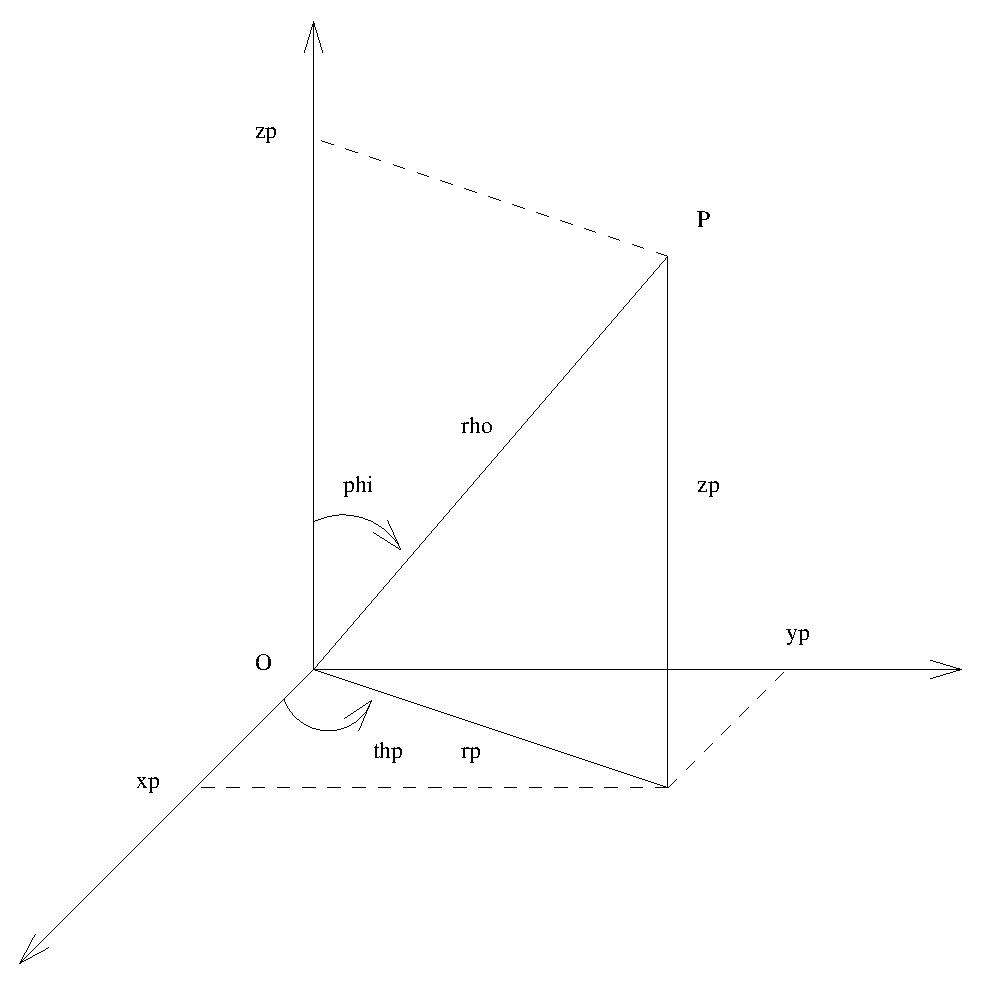
\includegraphics[height=2in]{../../modules/coordinate-systems/pictures/ok-cylindrical-spherical.eps}
\column{0.45\textwidth}
\begin{itemize}
\item In Cartesian coordinates, a point $P$ is given by triple $(x_P, y_P, z_P)$.
\item<2-> We introduce alternative spherical coordinates $(\rho_P, \phi_P,\theta_P)$.
\begin{itemize}
\item \alertNoH{3}{$\rho_P$: distance $|OP|$;}
\item \alertNoH{4}{$\phi_P$: angle $Oz$ to $OP$;}
\item \alertNoH{5}{$\theta_P$: angle $Ox$ to $OP_{xy}$.}
\end{itemize}
\item<6-> Coordinates range:
\begin{itemize}
\item \alertNoH{7,8}{$\rho$:} \uncover<8->{\alertNoH{8}{ $[0,\infty)$;}}
\item \alertNoH{9,10}{$\phi$:}  \uncover<10->{\alertNoH{10}{$[0, \pi]$;}}
\item \alertNoH{11,12}{$\theta$:}  \uncover<12->{ \alertNoH{12}{$[0,2\pi)$.}}
\end{itemize}
\end{itemize}
\end{columns}
\end{frame}

\begin{frame}
\frametitle{Transition Spherical - Rectangular coordinates}
\begin{columns}
\column{0.4\textwidth}
\psset{xunit=1cm, yunit=1cm}
\begin{pspicture}(-3,-2)(2,2)
\tiny
\renewcommand{\fcScreen}{[-1 -0.4 -0.25] -1}
\fcLineIIId[arrows=->]{[0 0 0]}{[5 0 0 ]}
\fcLineIIId[arrows=->]{[0 0 0]}{[0 5 0 ]}
\fcLineIIId[arrows=->]{[0 0 0]}{[0 0 5 ]}
\fcPutIIId[r]{[0 -0.15 0.15]}{\alert<2,3,4>{$O$}}
\fcLineIIId[linecolor=gray]{[3 0 0]}{[3 3 0]}
\fcLineIIId[linecolor=gray]{[3 3 0]}{[0 3 0]}
\fcLineIIId{[0 0 0]}{[3 3 0]}
\fcLineIIId{[3 3 0]}{[3 3 3]}
\fcLineIIId{[0 0 0]}{[3 3 3]}
\fcLineIIId{[0 0 3]}{[3 3 3]}
\fcPutIIId[l]{[3.1 3.1 3.1]}{\alert<4>{$P$}}
\fcPutIIId[r]{[1.5 -0.1 0]}{$\alert<1>{x}$}
\fcPutIIId[t]{[3.1 3.1 0]}{\alert<2,3>{$Q$}}
\uncover<2->{\fcPutIIId[l]{[1.4 1.5 0]}{\alert<4,5,6>{$~~r$}}}
\uncover<2->{
\fcPutIIId[r]{[3 -0.1 0]}{\alert<2,3>{$S$}}
\fcPolyLineIIId[linecolor=red]{[2.6 0 0 ] [2.6 0.4 0] [3 0.4 0]}
}
\uncover<2->{
\fcPutIIId[b]{[-0.1 1.5 0]}{$y$}
\fcPutIIId[t]{[3.1 1.5 0]}{\alert<5>{$y$}}
}
\uncover<7->{\fcPutIIId[r]{[0 0 1.5]}{\alert<7>{$z~~$}}}
\uncover<4->{
\fcPutIIId[r]{[0 -0.1 3]}{\alert<4>{$T~$}}
\fcPutIIId[b]{[1.4 1.5 3]}{\alert<4,6>{$~~r$}}
\fcPolyLineIIId[linecolor=red]{[2.6 2.6 0] [2.6 2.6 0.56569] [3 3 0.56569]}
\fcPolyLineIIId[linecolor=red]{[0.4 0.4 3] [0.4 0.4 3 0.56569 sub] [0 0 3 0.56569 sub]}
}
\fcPutIIId[r]{[1.7 1.7 1.7]}{\alert<4,6,7>{$\rho~~$}}
\fcPutIIId[rt]{[0.8 0.8 1.3]}{\alert<4,6,7>{$\phi~~$}}
\fcPutIIId[br]{[1.2 0.5 0]}{\alert<3,5>{$\theta$}}
\fcCurveIIId[linecolor=red, arrows=->]{0}{54.74}{ %
t sin 45 cos mul 1.5 mul % 
t sin 45 sin mul 1.5 mul %
t cos 1.5 mul %
} %
\fcCurveIIId[linecolor=red, arrows=->]{0}{45}{ %
t cos 1.5 mul % 
t sin 1.5 mul %
0 %
} %
\end{pspicture} 
\column{0.6\textwidth}

From spherical to rectangular coords:
\[
\begin{array}{rcll|l}
\alert<1->{x}&\alert<1>{=}& \uncover<3->{\alert<3>{ \alert<4>{r}\cos\theta}} &&\uncover<2->{\alert<2,5>{ \text{use }\triangle SQO}} \\ 
\uncover<4->{&\alert<0>{=} & \alert<4>{\rho\sin\phi }\cos\theta &&\alert<4,6,7>{ \text{use }\triangle OPT} }\\
\uncover<5->{\alert<5>{y}&\alert<0>{=}& \alert<5>{\alert<6>{r} \sin\theta } }\\
\uncover<6->{&\alert<0>{=}& \alert<6>{\rho\sin\phi }\sin\theta} \\
\uncover<7->{\alert<7>{z}&\alert<7>{=}& \alert<7>{\rho\cos\phi }}
\end{array}
\]
\uncover<8->{
From rectangular to spherical coords:
$$\rho = \sqrt{x^2+y^2+z^2} \quad , \quad r = \sqrt{x^2+y^2}$$
$$\cos\phi = \frac{z}{\rho} \quad , \quad \sin\phi = \frac{r}{\rho}$$
$$\cos\theta = \frac{x}{r} \quad , \quad \sin\theta = \frac{y}{r}$$
}
\end{columns}
\end{frame}

\begin{frame}
 \frametitle{Curvilinear boxes}
 
 Polar ``wedge'':
 %
$$C  = \{ P(r,\theta) \; | \;r_0 \leqslant
r \leqslant r_0+\Delta r,  \theta_0 \leqslant \theta
\leqslant \theta_0+\Delta \theta\} \; .$$
%
Shape? \pause Area = ...?
\pause

\bigskip

Cylindrical ``box'':
%
$$X = \{ P(r,\theta, z) \; | \; 0 \leqslant r \leqslant r_0\, ,
0 \leqslant \theta \leqslant \theta_0\, ,
0 \leqslant z \leqslant z_0\}$$

\pause
Shape ? \pause Volume = ...?

\bigskip

\pause
Spherical ``box'':
%
$$Y = \{ P(\rho, \phi, \theta) \; | \; 0 \leqslant \rho \leqslant \rho_0\, ,
0 \leqslant \phi \leqslant \phi_0\, ,
0 \leqslant \theta \leqslant \theta_0\}$$

\pause
Shape? \pause Volume = ...?

\end{frame}
}% end lecture

% begin lecture
\lect{2014}{Lecture  3}{3}{
\section{Vectors}
\begin{frame}
 \frametitle{Vectors}

\begin{itemize}
 \item Location of projector from current position and orientation:

\pause
\begin{itemize}
  \item direction of projector
  \item distance to projector
\end{itemize}

\pause
\item (direction, distance=magnitude) $\Longleftrightarrow$ \textit{vector}

\pause
\item Examples:
\begin{itemize}
  \item Force
  \item Velocity
  \item Displacement
\end{itemize}
\end{itemize}

\end{frame}
\begin{frame}
\frametitle{Displacement Vectors}
\begin{columns}\column{0.3\textwidth}
\begin{pspicture}(-0.2,-1.1)(2.1,1.1)
\fcBoundingBox{-0.2}{-1.1}{2.1}{1.1}
\fcFullDot{2}{1}
\fcFullDot{1}{-1}
\fcFullDotBlack{0}{0}
\psline(2, 1)(1,-1)
\psline[arrows=->](2, 1)(1,-1)
\end{pspicture}
\column{0.7\textwidth}
\begin{definition}
A displacement vector is an ordered pair of points, $(A,B)$.
\end{definition}
\end{columns}
\begin{itemize}
\item Represented as arrow, $A$ - tail $B$- head
\item Extra notation $(A,B) = \overrightarrow{AB} = \textbf{AB}$
\item Magnitude: $|\textbf{AB}| = |\overrightarrow{AB}|$. 
\item If $A\neq B$ direction is defined as the ray starting at $A$ and passing through $B$.
\item If $A=B$:
\begin{itemize}
\item Zero magnitude and non-specified direction
\item $(A,A) = \overrightarrow{AA} = \textbf{AA}$: zero displacement vector.
\end{itemize}
  \item Displacement vector with tail fixed at $O$:
  \begin{itemize}
    \item Position vector with respect to $O$;
    \item $(O,P) = \overrightarrow{OP} = \textbf{OP} = \textbf{r}_P$.
  \end{itemize}
\end{itemize}
\end{frame}
\begin{frame}
\frametitle{Equality and Equivalence of Displacement Vectors}
\begin{itemize}
\item<1-> We define two displacement vectors to be equal if:
\[ 
\textbf{AB} = \textbf{DC}  \Longleftrightarrow A=D \text{ and } B=C
\]
\item<2-> Equal displacement vectors $\rightarrow$ same magnitude and direction.
\item<3-> Same magnitude and direction $\not\rightarrow$ equal displacement vectors. 

\item<4-> We define two displacement vectors to be \alert<4>{equivalent} if they have the \alert<4>{same magnitude and direction}. We write $\alert<4>{\textbf{AB} \equiv \textbf{DC}}$.
\item 
\[ 
\textbf{AB} \equiv \textbf{DC} \Longleftrightarrow ABCD \text{ is a parallelogram}\;.
\]
\end{itemize}
\end{frame}
\begin{frame}
\frametitle{Position vectors}

  \begin{itemize}
   \item Vector $\textbf{u}$: \\
      set of displacement vectors with given direction and magnitude

    \item  Magnitude of $\textbf{u}$: common given magnitude.

    \item Direction of $\textbf{u}$: common given direction, if non-zero magnitude.

    \item Set of zero displacement vectors = zero vector, $\textbf{0}$. \pause

    \item Representative for $\textbf{u}$: \\
      displacement vector $\textbf{AB}$ with the same direction and magnitude

\begin{figure}[h]
  \psfrag{A}{$A$}
  \psfrag{B}{$B$}
  \psfrag{C}{$C$}
  \psfrag{D}{$D$}
  \psfrag{E}{$E$}
  \psfrag{F}{$F$}
  \psfrag{u}{$\textbf{u}$}
  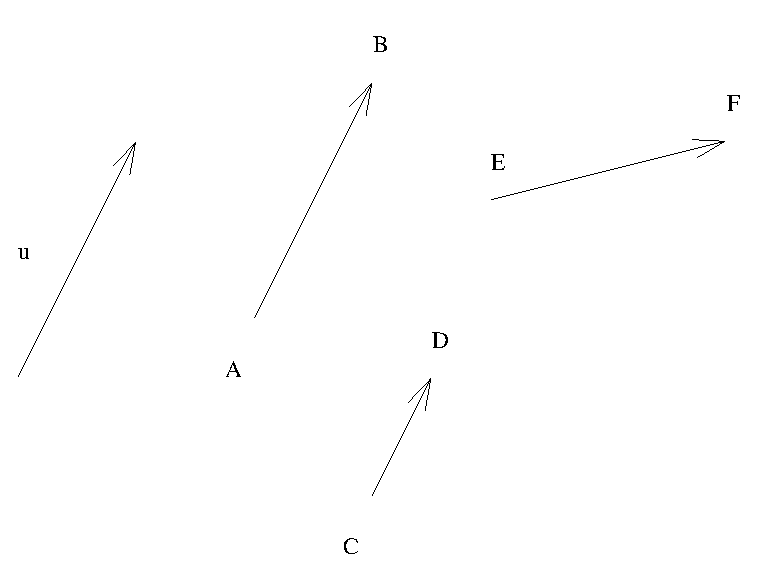
\includegraphics[height=1in]{../../modules/vectors/pictures/ok-vector_representatives.eps}
  \label{fig:vector_representative}

\end{figure}

    \item Intuitive notation:  $\textbf{u}=\textbf{AB}$.

    \item Graphical representation: arrow without fixed tail and head.

    %\item Major advantage: we can translate displacement vectors.
  \end{itemize}
\end{frame}
\begin{comment}
\begin{frame}
\frametitle{Addition of Vectors}
\begin{columns}
\column{0.25\textwidth}
\psset{xunit=1cm, yunit=1cm}
\begin{pspicture}(-0.5,-0.5)(3.1,3.1)%
\tiny
\fcBoundingBox{-0.5}{-0.5}{3.1}{3.1}
\uncover<1>{\psline[arrows=->](0,0)(1,2)}
\uncover<1>{%
\rput[r](0.4, 1){$\bm v$}%
}
\psline[arrows=->](0, 0)(2, 1)%
\rput[t](1, 0.4){$\bm u$}%
\uncover<2>{
\psline[linecolor=gray, arrows=->](0, 0)(1, 2)%
}
\uncover<2->{%
\psline[arrows=->](2,1)(3,3)%
\rput[l](2.6, 2){$\bm v$}}
\uncover<3->{%
\psline[arrows=->](0,0)(3,3)
\rput[rb](1.4,1.5){$\bm u+\bm v$}
}
\end{pspicture}

\column{0.75\textwidth}
\begin{itemize}
\item<1-> \textbf{Triangle Rule.} Define sum of position vectors $\bm u$ and $\bm v$ as follows. 
\item<2-> Attach representative displacement vectors head to tail.
\item<3-> Declare the sum to be the position vector with the tail of the first displacement vector and the head of the second displacement vector.
\end{itemize}
\end{columns}
\end{frame}

\begin{frame}
\frametitle{Properties of addition}
\begin{columns}
\column{0.4\textwidth}
\psset{xunit=1cm, yunit=1cm}
\begin{pspicture}(-0.5,-0.5)(3.1,3.1)%
\tiny
\fcBoundingBox{-0.5}{-0.5}{3.1}{3.1}
\uncover<2-4>{\psline[arrows=->, linecolor=red](0,0)(1,2)}
\uncover<5->{\psline[arrows=->](0,0)(1,2)}
\uncover<2->{\rput[r](0.4, 1){$\alert<2-4>{\bm v}$}}
\psline[arrows=->](2,1)(3,3)%
\uncover<1>{\psline[arrows=->, linecolor=red](2,1)(3,3)}
\rput[l](2.6, 2){$\alert<1>{\bm v}$}

\psline[arrows=->](0, 0)(2, 1)%
\uncover<1>{\psline[arrows=->, linecolor=red](0, 0)(2, 1)}
\rput[t](1, 0.4){$\alert<1>{\bm u}$}%
\uncover<3,4>{\psline[arrows=->, linecolor=red](1,2)(3,3)}
\uncover<5->{\psline[arrows=->](1,2)(3,3)}
\uncover<3->{\rput[b](2, 2.6){$\alert<3,4>{\bm u}$}}
\psline[arrows=->](0,0)(3,3)
\uncover<1,4>{
\psline[arrows=->, linecolor=red](0,0)(3,3)
}
\uncover<4->{\rput[t](1.62,1.62){\rotatebox{45}{$\alert<4>{ \bm v+\bm u}$}}}
\rput[b](1.38,1.38){\rotatebox{45}{$\alert<1>{\bm u+\bm v}$}}
\end{pspicture}

\uncover<5->{
\psset{xunit=0.8cm, yunit=0.8cm}
\begin{pspicture}(-0.5, -1)(4, 4)
\fcBoundingBox{-0.5}{-1}{4}{4}
\tiny

\uncover<5->{\psline[arrows=->](0,0)(0.5, 2) }
\uncover<6,9>{\psline[arrows=->, linecolor=red](0,0)(0.5,2)}
\rput[r](0.15,1){$\alert<6,9>{\bm u}$}

\uncover<5->{\psline[arrows=->](0.5, 2)(3, 3)}
\uncover<6,8>{\psline[arrows=->, linecolor=red](0.5,2)(3,3)}
\rput[b](1.75,2.6){$\alert<6,8>{\bm v}$}

\uncover<6->{\rput[tl](1.7, 1.7){\alert<6,7>{$\bm u+\bm v$}}}
\uncover<6,7>{\psline[arrows=->, linecolor=red](0,0)(3,3)}
\uncover<8->{\psline[arrows=->](0,0)(3,3)}

\uncover<7>{\psline[arrows=->, linecolor=red](3,3)(4,0)}

\uncover<5->{\psline[arrows=->](3, 3)(4, 0)}
\uncover<7,8>{\psline[arrows=->, linecolor=red](3, 3)(4, 0)}
\rput[lb](3.6,1.5){$\alert<7,8>{\bm w}$}

\uncover<7->{\rput[t](2, -0.1){\alert<6,7,10>{$(\bm u+\bm v )+\bm w$}}}
\uncover<9->{\rput[b](2, 0.1){\alert<9,10>{$\bm u+(\bm v +\bm w)$}}}
\uncover<8,11->{\psline[arrows=->](0, 0)(4, 0)}
\uncover<7,9,10>{\psline[arrows=->, linecolor=red](0, 0)(4, 0)}


\uncover<8->{\rput[tr](2.25, 1){$\alert<8,9>{\bm v+\bm w}$}}
\uncover<10->{\psline[arrows=->](0.5, 2)(4,0)}
\uncover<8,9>{\psline[arrows=->, linecolor=red](0.5, 2)(4,0)}

\end{pspicture}
}
\column{0.6\textwidth}
\begin{itemize}
\item Addition is commutative (parallelogram rule): \[ \alert<1>{\bm{u}+ \bm{v}} = \alert<4>{\alert<2>{\bm{v}}+ \alert<3>{\bm{u}}}.\]

\item<5-> Addition is associative: 
\[
\alert<10>{\alert<7>{(\alert<6>{ \bm{u}+\bm{v}})+\bm{w} } = \alert<9>{\bm{u} + (\alert<8>{ \bm{v} + \bm{w}})}}
\] 

\item<11-> As usual we write $\bm{u}+\bm{v}+\bm{w}=( \bm{u} +\bm{v})+\bm{w}= \bm{u}+(\bm{v}+\bm{w})$.
\end{itemize}
\end{columns}
\end{frame}
\end{comment}


\begin{frame}\frametitle{Difference of vectors}
\begin{columns}
\column{0.4\textwidth}
\psset{xunit=1cm, yunit=1cm}
\begin{pspicture}(-0.5,-2.5)(4.1,3.1)%
\fcBoundingBox{-0.5}{-2.5}{4.1}{3.1}
\uncover<1,2,6>{\rput[b](1, 0.6){$\bm u$}}
\uncover<1,2,6>{\psline[arrows=->](0,0)(2,1)}
\uncover<3>{\psline[arrows=->, linecolor=red](0,0)(2,1)}

\uncover<3-4,7->{\psline[arrows=->, linecolor=red](2,1)(0,0)}
\uncover<5>{\psline[arrows=->](2,1)(0,0)}
\uncover<3>{\rput[lt](1,0.5){$\alert<3>{-\bm u=\bm{BA}}$}}
\uncover<4-5,7->{\rput[lt](1,0.5){$\alert<4,7>{-\bm u}$}}
\uncover<3>{\fcFullDot{0}{0}}
\uncover<6>{\psline[arrows=->](0,0)(1,-2)}
\uncover<7>{\psline[arrows=->, linecolor=red](0,0)(1,-2)}
\uncover<6->{\rput[tr](0.5, -1){$\alert<7>{\bm v}~$}}
\uncover<7->{\psline[arrows=->, linecolor=red](2, 1)(1,-2)}
\uncover<7->{\rput[l](1.5,-0.5){$~\alert<7>{\bm v-\bm u}$}}
\uncover<1-5>{
\rput[tl](0,-0.1){$A$}
\rput[tl](2,0.9){$B$}
}
\end{pspicture}
\column{0.6\textwidth}
\begin{itemize}
\item Let $\bm u=\bm{AB}$. 
\item<2-> We define $-\bm u$ to be \uncover<5->{\alert<5>{the}} \uncover<1-4>{a} vector for which $\bm u +(-\bm u)=\bm 0 $. 
\item<3-> Since $\bm{AB} + \bm{BA} = \bm{0}$, it follows $\alert<3>{-\bm u=\bm {BA}}$.
\item<4-> In other words $-\bm{u}$ is depicted using the arrow opposite to $\bm u$.
\item<5-> From picture, it's evident \alert<5>{$-\bm u $ can be chosen in a only one way}.
\item<6-> We define the difference of vectors $\bm v, \bm u$ via \uncover<7->{$\alert<7>{\bm{v}-\bm{u}= (-\bm{u})+ \bm{v} } $ (triangle rule)}.
\end{itemize}
\end{columns}
\end{frame}
\begin{frame}
\frametitle{Linear Combinations}
\begin{columns}
\column{0.3\textwidth}
\psset{xunit=0.6cm, yunit=0.6cm}
\begin{pspicture}(-2,-2)(3.1,3.3)
\fcBoundingBox{-2}{-2}{3}{3}
\fcFullDot{0}{0}
\rput[br](3, 3){$\fcv u$}
\psline[arrows=->](0,0)(3,3)
\uncover<handout:0|3>{
\psline[arrows=->, linecolor=red](0,0)(1.5,1.5)
\rput[tl](0.75, 0.75){$\alertNoH{3}{\frac{1}{2}\fcv u}$}
}
\uncover<4>{
\psline[arrows=->, linecolor=red](0,0)(2,2)
\rput[tl](1, 1){$\alertNoH{4}{\frac{2}{3}\fcv u}$}
}
\uncover<handout:0|5>{
\psline[arrows=->, linecolor=red](0,0)(1,1)
\rput[tl](0.5, 0.5){$\alertNoH{5}{\frac{1}{3}\fcv u}$}
}
\uncover<6>{
\psline[arrows=->, linecolor=red](0,0)(-2,-2)
\rput[tl](-1, -1){$\alertNoH{6}{-\frac{1}{2}\fcv u}$}
}
\end{pspicture}
\column{0.7\textwidth}
\begin{itemize}
\item<1-> Let $\fcv{u}$ be vector, $c$ be a real number (scalar).
\item<2-> Define \alertNoH{2}{the product of the vector $\fcv u$ and the scalar $c$} as follows.
\begin{itemize}
\item<2-> If $c >0$ define $c\fcv{u}$ as the vector:
\begin{itemize}
\item with the same direction
\item with magnitude proportional with coefficient $c$ to the magnitude of $\fcv u$, i.e., $|c\fcv{u}| = c|\fcv{u}|$.
\end{itemize}

\item<6-> If $c<0$ define $c\fcv{u}$ as the vector $(-c)(-\fcv{u})$, i.e, as the vector:
\begin{itemize}
\item with opposite direction
\item with magnitude $|c\fcv{u}| = |(-c)(-\fcv{u})| = (-c)|-\fcv{u}| = |c||\fcv{u}|$
\end{itemize}
\item<7-> If $c=0$ then define $c\fcv u=0\fcv{u} = \fcv{0}$.
\end{itemize}
\end{itemize}
\end{columns}
\begin{itemize}
\item If $c_1, \ldots , c_n$ are scalars and $\fcv{u}_1,\ldots, \fcv{u}_n$ are vectors, we say
\[
\fcv{v} = c_1\fcv{u}_1+ \dotsb + c_n \fcv{u}_n
\]
is a \emph{linear combination} of the vectors $\fcv u_1,\dots, \fcv u_n$.
\end{itemize}
\end{frame}
\begin{frame}
  \frametitle{Decomposition of a vector along given directions}

  Example: Tension induced by given force.

\begin{figure}[h]
  \psfrag{F}{$\textbf{F}$}
  \psfrag{-F}{$-\textbf{F}$}
  \psfrag{F1}{$\textbf{F}_1$}
  \psfrag{F2}{$\textbf{F}_2$}
  \psfrag{T1}{$\textbf{T}_1$}
  \psfrag{T2}{$\textbf{T}_2$}
  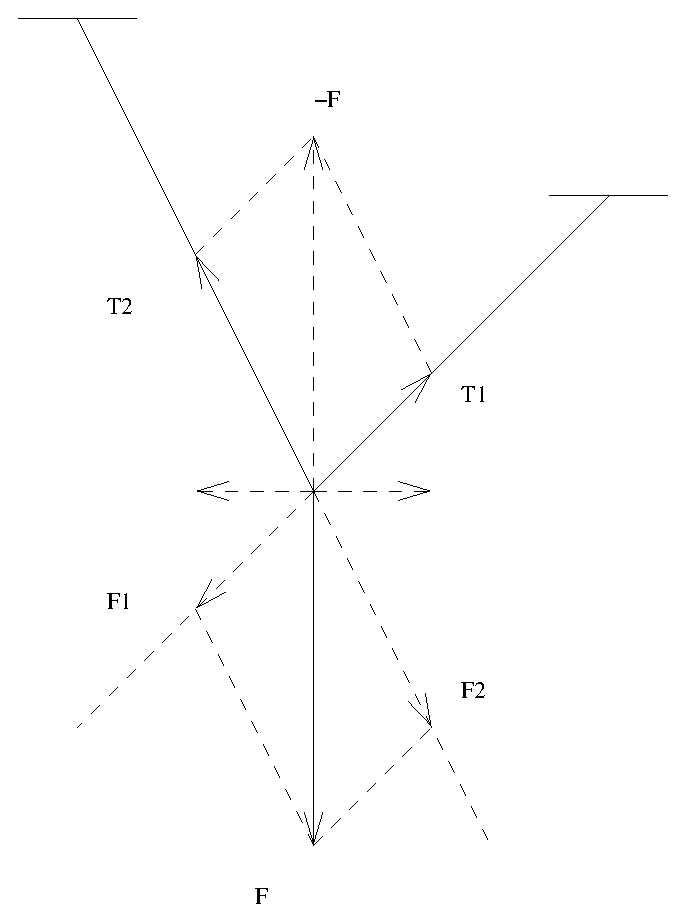
\includegraphics[height=2in]{../../modules/vectors/pictures/ok-tension.eps}
  \label{fig:tension}
  %\caption{Decomposition of a vector}
\end{figure}


\end{frame}
%\begin{comment}
\begin{frame}
\frametitle{Vectors in Coordinates}
\begin{columns}
\column{0.3\textwidth}
\psset{xunit=0.7cm, yunit=0.7cm}
\begin{pspicture}(-0.5 ,-2)(4.5, 4)
\fcBoundingBox{-0.5}{-2}{4.5}{4}
\tiny
\renewcommand{\fcScreen}{[-1 1.1 -0.5] 0}
\fcAxesIIId{3}{3}{3}
\fcPutIIId[r]{[0 0 0]}{$O~$}
\uncover<3->{
\fcLineIIId[arrows=->, linecolor=red]{[0 0 0]}{[1 0 0]}
\fcLineIIId[arrows=->, linecolor=red]{[0 0 0]}{[0 1 0]}
\fcLineIIId[arrows=->, linecolor=red]{[0 0 0]}{[0 0 1]}
\fcPutIIId[t]{[0.5 0 -0.1]}{$\alert<3>{\bm i}$}
\fcPutIIId[br]{[0 0.5 0]}{$\alert<3>{\bm j}$}
\fcPutIIId[r]{[0 0 0.5]}{$\alert<3>{\bm k}~~$}
}
\uncover<5->{
\fcPutIIId[lb]{[2.5 2.5 2.8]}{$U\uncover<6->{(a,b,c)}$}
\fcDotIIId[linecolor=blue]{[2.5 2.5 2.5]}%
\fcLineIIId[arrows=->, linecolor=red]{[0 0 0]}{[2.5 2.5 2.5]}
}
\uncover<2,3>{
\fcDotIIId{[1 0 0]}
\fcDotIIId{[0 1 0]}
\fcDotIIId{[0 0 1]}
}
\uncover<2>{
\fcPutIIId[t]{[1 0 -0.2]}{\alert<2>{$I$}}
\fcPutIIId[br]{[0 1 0]}{\alert<2>{$J~~$}}
\fcPutIIId[r]{[0 0 1]}{\alert<2>{$K~~$}}
}
\uncover<6,11>{
\fcLineIIId[linecolor=gray]{[2.5 2.5 2.5]}{[2.5 2.5 0]}
\fcLineIIId[linecolor=gray]{[2.5 2.5 2.5]}{[2.5 0 2.5]}
\fcLineIIId[linecolor=gray]{[2.5 2.5 2.5]}{[0 2.5 2.5]}
\fcLineIIId[linecolor=gray]{[0 2.5 2.5]}{[0 0 2.5]}
\fcLineIIId[linestyle=dashed, linecolor=gray]{[0 2.5 2.5]}{[0 2.5 0]}
\fcLineIIId[linecolor=gray]{[2.5 0 2.5]}{[0 0 2.5]}
\fcLineIIId[linecolor=gray]{[2.5 0 2.5]}{[2.5 0 0]}
\fcLineIIId[linestyle=dashed, linecolor=gray]{[2.5 2.5 0]}{[0 2.5 0]}
\fcLineIIId[linecolor=gray]{[2.5 2.5 0]}{[2.5 0 0]}%
}
\uncover<6>{
\fcPutIIId[t]{[1.25 0 -0.1]}{$a$}
\fcPutIIId[b]{[0 1.25 0.1]}{$b$}%
\fcPutIIId[r]{[0 0 1.25]}{$c~~$}%
}
\uncover<8->{
\fcPutIIId[t]{[1.25 0 -0.1]}{$a\bm{i}$}
\fcLineIIId[arrows=->, linecolor=red]{[0 0 0]}{[2.5 0 0]}
}
\uncover<9->{
\fcLineIIId[arrows=->, linecolor=red]{[2.5 0 0]}{[2.5 2.5 0]}
\fcPutIIId[lt]{[2.5 1.25 0]}{$~b\bm{j}$}%
}
\uncover<10->{
\fcLineIIId[arrows=->, linecolor=red]{[2.5 2.5 0]}{[2.5 2.5 2.5]}
\fcPutIIId[l]{[2.5 2.5 1.25]}{$~c\bm{k}$}%
}
\end{pspicture}
\column{0.7\textwidth}
\begin{itemize}
\item<1-> Fix coordinate system $Oxyz$.
\item<2-> Let $I$, $J$, $K$ be the points giving the units on the $x,y,z$ axes as indicated.
\item<3-> Define $\bm{i}$, $\bm{j}$, $\bm{k}$ to be the unit vectors $\bm{OI}$, $\bm{OJ}$, $\bm{OK}$.
\end{itemize}
\end{columns}
\begin{itemize}
\item<5-> Let $\bm u= \bm{OU}$ be a vector.
\item<6-> Let $U$ have coordinates $(a,b,c)$.
\item<7-> Then $\bm u =\alert<10>{ \alert<9>{\alert<8>{ a\bm{i}}+b\bm{j}}+c\bm{k} }$.
\item<8-11> This follows from the point-vector identification.
\end{itemize}
\end{frame}
%\end{comment}
\begin{frame}
\begin{columns}
\column{0.3\textwidth}
\psset{xunit=0.7cm, yunit=0.7cm}
\begin{pspicture}(-0.5 ,-2)(4.5, 4)
\fcBoundingBox{-0.5}{-2}{4.5}{4}
\tiny
\renewcommand{\fcScreen}{[-1 1.1 -0.5] 0}
\fcAxesIIId{3}{3}{3}
\fcPutIIId[r]{[0 0 0]}{$O~$}
\fcLineIIId[arrows=->, linecolor=red]{[0 0 0]}{[1 0 0]}
\fcLineIIId[arrows=->, linecolor=red]{[0 0 0]}{[0 1 0]}
\fcLineIIId[arrows=->, linecolor=red]{[0 0 0]}{[0 0 1]}
\fcPutIIId[t]{[0.5 0 -0.1]}{$\alert<3>{\bm i}$}
\fcPutIIId[br]{[0 0.5 0]}{$\alert<3>{\bm j}$}
\fcPutIIId[r]{[0 0 0.5]}{$\alert<3>{\bm k}~~$}
\fcPutIIId[lb]{[2.5 2.5 2.8]}{$U(a,b,c)$}
\uncover<2->{\fcPutIIId[rb]{[1.25 1.25 1.3]}{$\bm u( a,b,c)$}}
\fcDotIIId[linecolor=blue]{[2.5 2.5 2.5]}%
\fcLineIIId[arrows=->, linecolor=red]{[0 0 0]}{[2.5 2.5 2.5]}
\fcPutIIId[t]{[1.25 0 -0.1]}{$a\bm{i}$}
\fcLineIIId[arrows=->, linecolor=red]{[0 0 0]}{[2.5 0 0]}
\fcLineIIId[arrows=->, linecolor=red]{[2.5 0 0]}{[2.5 2.5 0]}
\fcPutIIId[lt]{[2.5 1.25 0]}{$~b\bm{j}$}%
\fcLineIIId[arrows=->, linecolor=red]{[2.5 2.5 0]}{[2.5 2.5 2.5]}
\fcPutIIId[l]{[2.5 2.5 1.25]}{$~c\bm{k}$}%
\end{pspicture}
\column{0.7\textwidth}
\begin{itemize}
\item<1-> From preceding: arbitrary vector $\bm u= \bm {OU}$ can be decomposed as $\bm u= a\bm i+b\bm j + c\bm k$, where $(a,b,c)$: Cartesian coordinates of $U$.
\item<2-> Thus $\bm u$ is identified with the triple of numbers $( a, b, c)$.
\end{itemize}
\end{columns}

\begin{itemize}
\item<3-> Under the first definition of vector, a vector is simply a point in a vector space (=space with a distinguished point).
\item<4-> From now on, we assume the first definition of vector: we use the notation $(a,b,c)$ both for points in vector spaces (vectors) and points in spaces not equipped with vector space structure.
\item<5-> Under the second alternative definition of vector, there is a formal distinction between points and vectors.
\item<6-> Some authors who use the second definition use the notation $\langle a, b, c \rangle$ to denote vectors and $(a,b,c)$ to denote points.
\end{itemize}
\end{frame}

\begin{frame}
\frametitle{Work done by a constant force}
\only<1>{
\begin{figure}[h]
  \psfrag{F}{$\textbf{F}$}
  \psfrag{O}{$O$}
  \psfrag{P}{$P$}
  \psfrag{a}{$\alpha$}
  \psfrag{pvF}{$\textbf{proj}_{\bm{v}} \textbf{F}$}
  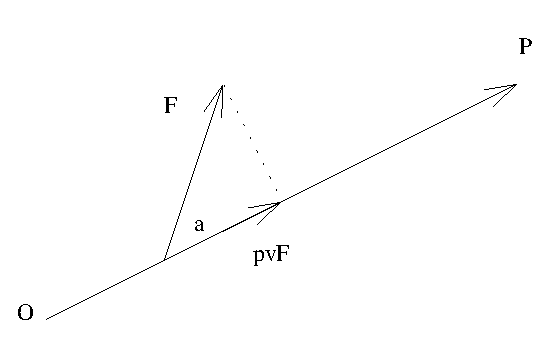
\includegraphics[height=2in]{../../modules/vectors/pictures/ok-positive_work.eps}
\end{figure}

$$W = |\textbf{proj}_{\bm{v}} \textbf{F}| \, |\textbf{OP}| =|\textbf{F}| \, |\textbf{OP}|\, \cos{\alpha}\; .$$
}

\only<2>{
\begin{figure}[h]
  \psfrag{F}{$\textbf{F}$}
  \psfrag{O}{$O$}
  \psfrag{P}{$P$}
  \psfrag{a}{$\alpha$}
  \psfrag{pvF}{$\textbf{proj}_{\bm{v}} \textbf{F}$}
  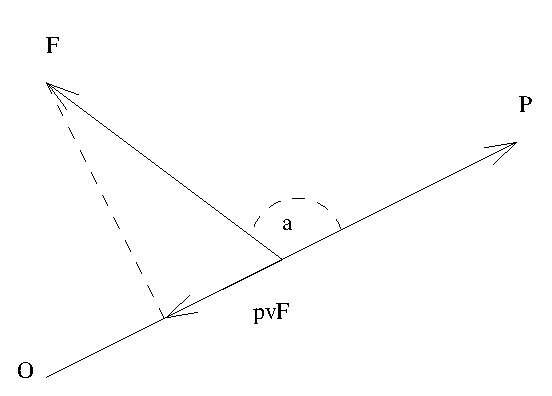
\includegraphics[height=2in]{../../modules/vectors/pictures/ok-negative_work.eps}
\end{figure}

$$W = - |\textbf{proj}_{\bm{v}} \textbf{F}| \, |\textbf{OP}| = |\textbf{F}| |\textbf{OP}| \cos{\alpha}\; .$$
}

\end{frame}


\begin{frame}
\frametitle{Dot Product}
\begin{columns}
\column{0.5\textwidth}
\begin{pspicture}(-0.5, -0.5)(5,3.2)
\fcBoundingBox{-0.5}{-0.5}{5}{3.2}
\psline[arrows=->](0,0)(4, 2)
\rput[tl](3, 1.5){$\bm v$}
\rput[tl](0.5, 0.2){$\hat{ \bm {v}}$}
\rput[bl](1, 3){$ \bm u$}
\rput[r](-0.5, 1){$\textbf{orth}_{\bm v} \bm u$}

\rput[r](-0.5, 1){$\textbf{orth}_{\bm v} \bm u$}
\rput[tl](1.5, 0.8){$\textbf{proj}_{\bm v} \bm u$}

\psline[arrows=->](0,0)(2,1)
\psline[arrows=->, linecolor=red](0,0)(! 4 20 sqrt div 2 20 sqrt div)

\psline[arrows=->](0,0)(1,3)
\psline[arrows=->](0,0)(! -1 2)
\fcPerpendicular[linestyle=dashed]{[1 3]}{[4 2]}{0.2}%
\fcPerpendicular[linestyle=dashed]{[1 3]}{[-2 4]}{0.2}%
\fcAngle{0.463648}{ 1.249046 }{0.4}{$\alpha$}
\end{pspicture}
\column{0.5\textwidth}

\begin{itemize}
\item<1-> Let $\bm{u}$, $\bm{v}$ vectors, $\bm{v}\neq \bm{0}$.

\item<2-> Let $\textbf{proj}_{\bm{v}} \bm{u}$: projection of $\bm{u}$ along $\bm{v}$.

\item<3-> Let $\textbf{orth}_{\bm{v}} \bm{u}$: projection of $\bm{u}$ orthogonal to $\bm{v}$.

\item<4-> Then $\hat{\bm{v}} = \frac{1}{|\bm{v}|} \bm{v}$ is the unit vector along $\bm{v}$.

\item<5-> Let $\alpha$: angle between $\bm v$ and $\bm u$.

\item<6-> Then $\textbf{proj}_{\bm{v}} \bm{u} =  \cos \alpha |\bm{u}| \hat{\bm{v}}$.

\item<7-> Define dot product of $u$ and $v$:
\[
\bm{u} \cdot \bm{v} =  \cos \alpha |\bm u||\bm{v}| .
\]
\end{itemize}
\end{columns}
\end{frame}

\begin{frame}
 \frametitle{Properties of Dot Product}

  \begin{itemize}
   \item If $\textbf{v}=\textbf{0}$ or $\textbf{u}=\textbf{0}$, then $\textbf{u}\cdot \textbf{v} =0$.

  \item If $\textbf{u} \neq 0 \neq \textbf{v}$, then $comp_{\bm{v}} \textbf{u} = |\textbf{u}|\cos{\alpha}$
%
$$\textbf{u} \cdot \textbf{v} = |\textbf{u}| \, |\textbf{v}|\,\cos{\alpha}$$
%
\item If $\textbf{u}\neq \textbf{0} \neq \textbf{v}$, then
%
$$\textbf{u} \cdot \textbf{v} = 0 \Longleftrightarrow \textbf{u} \bot \textbf{v}\; .$$
%
\item $\textbf{u} \cdot \textbf{v} = (\textbf{proj}_{\bm{v}} \textbf{u}) \cdot \textbf{v}$

\item The dot product is linear in each argument:
%
$$ (a \textbf{u} + b \textbf{w}) \cdot \textbf{v} = a \textbf{u} \cdot \textbf{v} + b \textbf{w} \cdot \textbf{v}$$
%
$$ \textbf{u} \cdot (a \textbf{v} + b \textbf{w}) = a \textbf{u} \cdot \textbf{v} + b \textbf{u} \cdot \textbf{w}$$

\item Dot product is positive definite:
%
$$\textbf{v} \cdot \textbf{v} = |\textbf{v}|^2 \geqslant 0 \text{ and }
\textbf{v}\cdot \textbf{v} = 0 \leftrightarrow \textbf{v}=\textbf{0}$$
  \end{itemize}

\end{frame}
\begin{frame}
 \frametitle{Computations in Coordinates}

 \begin{itemize}
  \item  $Oxyz$: rectangular coordinate system

  \item $\textbf{i}$, $\textbf{j}$, $\textbf{k}$: unit vectors along fundamental directions.
%
$$ \textbf{i} \cdot \textbf{j} = \textbf{j} \cdot \textbf{i} = \textbf{j} \cdot \textbf{k}
 = \textbf{k} \cdot \textbf{j} = \textbf{i} \cdot \textbf{k} = \textbf{k} \cdot \textbf{i} = 0$$
%
$$\textbf{i} \cdot \textbf{i} = \textbf{j} \cdot \textbf{j} = \textbf{k} \cdot \textbf{k} = 1$$

  \item $\textbf{u} = u_1 \textbf{i} + u_2 \textbf{j} + u_3 \textbf{k} = \langle u_1, u_2, u_3 \rangle$,
 $\textbf{v}=v_1 \textbf{i} + v_2 \textbf{j} + v_3 \textbf{k} = \langle v_1, v_2, v_3 \rangle$,
%
$$\textbf{u} \cdot \textbf{v} = \langle u_1, u_2, u_3 \rangle \cdot \langle v_1, v_2, v_3 \rangle =
u_1v_1 + u_2 v_2 +u_3 v_3\; .$$

\item Example: $\langle 1,2,3 \rangle \cdot \langle 6,5,4 \rangle = 1 \cdot 6 + 2\cdot 5 + 3 \cdot 4 = 28$.
 \end{itemize}
\end{frame}

\begin{frame}
\frametitle{Projections in coordinates}
\begin{columns}
\column{0.4\textwidth}
\psset{xunit=0.6cm, yunit=0.6cm}
\begin{pspicture}(-2, -0.5)(5,3.2)
\fcBoundingBox{-2}{-0.5}{5}{3.2}%
\psline[arrows=->](0,0)(4, 2)%
\rput[tl](3, 1.5){$\fcv v$}%
\rput[bl](1, 3){$ \fcv u$}%
\psline[arrows=->, linecolor=blue](0,0)(2,1)%
\rput[tl](1.5, 0.8){$\textbf{proj}_{\fcv v} \fcv u$}%
\psline[arrows=->, linecolor=red](0,0)(! 4 20 sqrt div 2 20 sqrt div)%
\rput[tl](0.5, 0.1){$\widehat{ \fcv {v}}$}%
\psline[arrows=->](0,0)(1,3)%
\fcPerpendicular[linestyle=dashed]{[1 3]}{[4 2]}{0.2}%
\end{pspicture}
\column{0.6\textwidth}
\[
\begin{array}{rcl}
\fcv{u} &=& u_1 \fcv{i} + u_2 \fcv{j} + u_3 \fcv{k} = \langle u_1, u_2, u_3 \rangle\\
\fcv{v}&=&v_1 \fcv{i} + v_2 \fcv{j} + v_3 \fcv{k} = \langle v_1, v_2, v_3 \rangle
\end{array}
\]
\end{columns}
\uncover<2->{
\begin{theorem}
$\begin{array}{rcl}
\displaystyle\alert<6>{ {\bf comp}_{\fcv v} \fcv u}&\alert<6>{=}& \displaystyle \alert<6>{\frac{\alert<3>{\fcv{u}\cdot \fcv{v}} }{\alert<4>{|\fcv{v}|}}} =\frac{ \alert<3>{ u_1v_1 +u_2v_2+u_3v_3} }{\alert<4>{ \sqrt{v_1^2+v_2^2+v_3^2}}}\\~\\
\displaystyle \alert<5>{{\bf proj}_{\fcv v} \fcv u }&\alert<-1>{=}&\displaystyle \alert<5>{\left(\alert<6>{ {\bf comp}_{\fcv v} \fcv{u}}\right) \alert<7>{\widehat{\fcv v}}} = \alert<6>{\frac{\fcv{u}\cdot \fcv{v}}{|\fcv{v}|}} \alert<7>{ \frac{\fcv v}{|\fcv v|}} = \frac{\fcv{u}\cdot \fcv{v}}{\alert<8>{ |\fcv{v}|^2}}\fcv v= \frac{\fcv u \cdot \fcv v}{\alert<8>{ \fcv v\cdot  \fcv v} }\fcv v
\quad .
\end{array}
$
\end{theorem}
}
\end{frame}

\begin{frame}
 \frametitle{Angles}

$$\cos{\alpha} = \frac{\textbf{u} \cdot \textbf{v}}{|\textbf{u}|\, |\textbf{v}|} \to \alpha =
\arccos{\left( \frac{\textbf{u} \cdot \textbf{v}}{|\textbf{u}|\, |\textbf{v}|} \right)}$$

Example:

\bigskip

Angle between $\langle 1,2,3\rangle$ and $\langle 6,5,4\rangle$:
%
$$\alpha = \arccos{\left( \frac{28}{\sqrt{14}\, \sqrt{77}} \right)} =
\arccos{\left( \frac{4}{\sqrt{22}} \right)}$$

\end{frame}

\begin{frame}
 \frametitle{Direction Angles}

\begin{figure}[h]
  \psfrag{u}{$\textbf{u}$}
  \psfrag{i}{$\textbf{i}$}
  \psfrag{j}{$\textbf{j}$}
  \psfrag{k}{$\textbf{k}$}
  \psfrag{a}{$\alpha$}
  \psfrag{b}{$\beta$}
  \psfrag{c}{$\gamma$}
  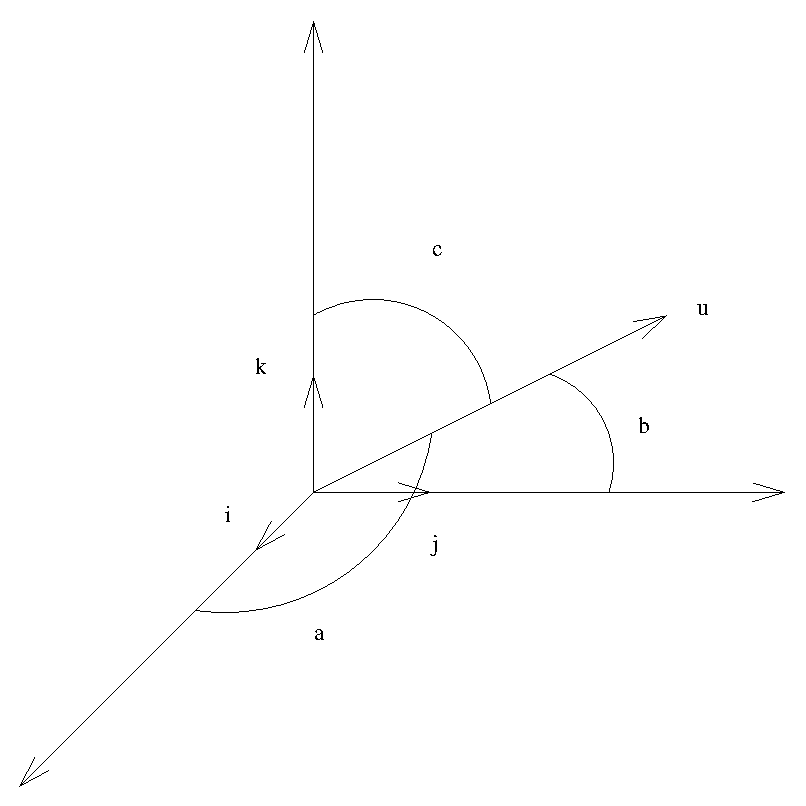
\includegraphics[height=2in]{../../modules/vectors/pictures/ok-direction_angles.eps}
\end{figure}


$\textbf{u} = \langle u_1, u_2, u_3\rangle, \qquad \alpha = \angle (\textbf{u},\textbf{i}) \qquad \beta =
\angle (\textbf{u},\textbf{j}) \qquad \gamma = \angle (\textbf{u},\textbf{k}) \; .$

$$\cos{\alpha} = \frac{\textbf{u} \cdot \textbf{i}}{|\textbf{u}|\, |\textbf{i}|} =
\frac{u_1}{\sqrt{u_1^2+u_2^2+u_3^2}}$$

Similar for $\cos{\beta}$ and $\cos{\gamma}$. Then:
%
$$\cos^2\alpha + \cos^2\beta + \cos^2\gamma = 1\; .$$

\end{frame}

\begin{frame}
 \frametitle{Rotational Effect}

 \begin{itemize}
  \item Rigid rod $OP$, fixed at $O$, $\textbf{r}=\textbf{OP}$. Force $\textbf{F}$ applied at $P$.
 \end{itemize}
%
\begin{figure}[h]
  \psfrag{F}{$\textbf{F}$}
  \psfrag{r}{$\textbf{r}$}
  \psfrag{O}{$O$}
  \psfrag{P}{$P$}
  \psfrag{}{$\alpha$}
  \psfrag{pfr}{$\textbf{proj}_{\bm{r}} \textbf{F}$}
  \psfrag{ofr}{$\textbf{orth}_{\bm{r}} \textbf{F}$}
  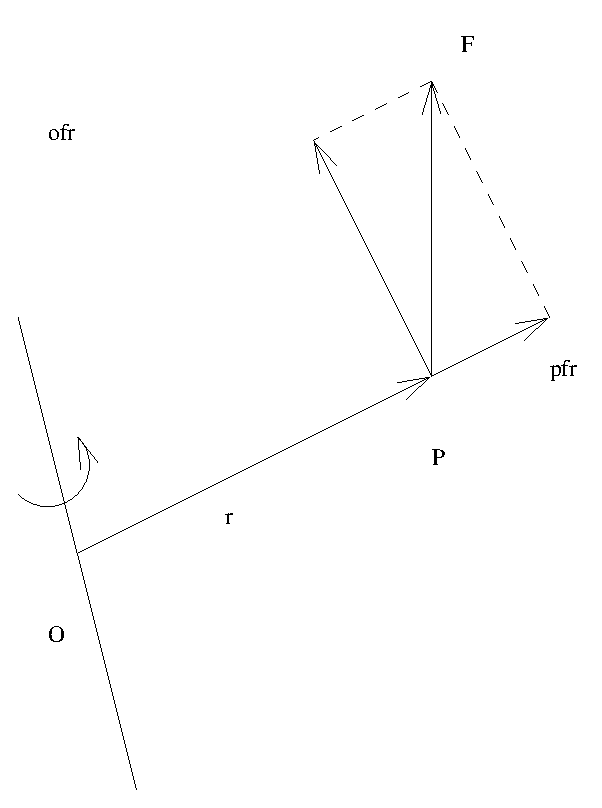
\includegraphics[height=1.5in]{../../modules/vectors/pictures/ok-torque.eps}
\end{figure}
%
\pause
\begin{itemize}
  \item $\textbf{proj}_{\bm{r}} \textbf{F}$: \pause no effect;
  \item $\textbf{orth}_{\bm{r}} \textbf{F}$: \pause rotational effect:\pause
  \begin{itemize}
    \item Axis of rotation: \pause perpendicular to $\textbf{r}$ and $\textbf{F}$;\pause
    \item Angular velocity: \pause proportional to $|\textbf{orth}_{\bm{r}} \textbf{F}|$;\pause
    \item Linear velocity: \pause proportional to $|\textbf{r}| \, |\textbf{orth}_{\bm{r}} \textbf{F}|$.
  \end{itemize}
\end{itemize}

\end{frame}
\begin{frame}
\frametitle{Torque}

Rotation in space $\Longleftrightarrow$ vector\pause
  \begin{itemize}
   \item Axis of rotation $\Longleftrightarrow$ Support of direction \pause
   \item Sense of rotation  $\Longleftrightarrow$ Direction of vector \pause
  \begin{itemize}
      \item Convention: Right Hand Rule\pause
  \end{itemize}
  \item Angular velocity $\Longleftrightarrow$ (proportional to) Magnitude of vector\pause
  \end{itemize}
\begin{center}
 $(\textbf{r}, \textbf{F}) \rightarrow$ rotation $\rightarrow$ vector = torque, $\bm{\tau}$
\end{center}



\begin{itemize}
 \item Support of direction: perpendicular to $\textbf{r}$ and $\textbf{F}$;
 \item Direction: Right Hand Rule;
 \item Magnitude: $|\bm{\tau}| = |\textbf{r}| \, |\textbf{orth}_{\bm{r}} \textbf{F}|$
\end{itemize}

\end{frame}
\begin{frame}
\frametitle{The Cross Product $\times$}
\begin{columns}
\column{0.35\textwidth}
\psset{xunit=2cm, yunit=2cm}
\begin{pspicture}(-0.2,-0.2)(1.2,1.2)
\tiny
\renewcommand{\fcScreenStyle}{[0 0.1 1]}%
\only<5->{\renewcommand{\fcScreen}{[-1 1 -0.5] 0}}%
\only<6->{\renewcommand{\fcScreen}{[-0.8 0.8 -0.5] 0}}%
\only<7->{\renewcommand{\fcScreen}{[-0.6 0.6 -0.5] 0}}%
\only<8->{\renewcommand{\fcScreen}{[-0.4 0.4 -0.5] 0}}%
\only<9->{\renewcommand{\fcScreen}{[-0.2 0.2 -0.5] 0}}%
\only<10->{\renewcommand{\fcScreen}{[-0.1 0.1 -0.5] 0}}%
\only<11->{\renewcommand{\fcScreen}{[-0.05 0.05 -0.5] 0}}%
\fcLineIIId[arrows=->]{[0 0 0]}{[1 0 0]}
\fcLineIIId[arrows=->]{[0 0 0]}{[1 1 0]}
\fcLineIIId[arrows=->]{[0 0 0]}{[0 0 1]}
\fcPutIIId[r]{[0 0 1]}{$\fcv u \times \fcv v$}
\fcAngleIIId[arrows=->, linecolor=blue]{[1 0 0]}{[1 1 0]}{0.4}
\fcPutIIId[lt]{[0.4 0.2 0]}{$\alpha$}
\fcPutIIId[t]{[1 0 -0.1]}{$\fcv u$}
\fcPutIIId[t]{[1 1 -0.1]}{$\fcv v$}
\uncover<3->{%
\fcLineIIId[arrows=->]{[0 0 0]}{[0 1 0]}
\fcPutIIId[rb]{[0 1 0]}{$\textbf{orth}_{\fcv u} \fcv v$}%
\fcPerpendicularIIId[linestyle=dashed]{[1 1 0]}{[0 1 0]}{0.2}%
}%
\only<2>{\fcPerpendicularIIId{[0 0 1]}{[-1 -1 0]}{0.2}%
\fcPerpendicularIIId{[0 0 1]}{[-1 0 0]}{0.2}%
}%
\end{pspicture}
\column{0.65\textwidth}

\begin{definition}[Cross product]
$\fcv{u} \times \fcv{v}$ is the vector uniquely determined by the following.
\begin{itemize}
\item If $\fcv{u}$, $\fcv{v}$ are non-zero and non-collinear.
\begin{itemize}
\item \alert<2>{ $\fcv{u} \times \fcv{v}$ is perpendicular to both $\fcv{u}$ and $\textbf{v}$.}
\item The magnitude of $\fcv{u} \times \fcv{v}$ equals $|\fcv{u}| \alert<3>{| \textbf{orth}_{\fcv u} \fcv v |}=|\textbf{u}| \alert<3>{|\textbf{v}| \sin{\alpha}}$.
\item \alert<4-12>{The direction of $\textbf{u} \times \textbf{v}$ is such that when viewed from the tip of $\fcv{u}\times \fcv v$, $\fcv v$ is counter-clockwise from $\fcv u$.}
\end{itemize}
\item If $\fcv{u}$, $\fcv{v}$ are colinear or zero then $\fcv u \times \fcv v=\fcv 0$.
\end{itemize}
\end{definition}
\end{columns}
\uncover<12->{\alert<12>{There are a couple of hand rules to help figure out the direction of the cross product.}}
\end{frame}
\begin{frame}
 \frametitle{Properties of Cross Product}
Let $\textbf{u}$, $\textbf{v}$ non-zero vectors, $\alpha = \angle(\textbf{u},\textbf{v})$.


\begin{itemize}
\item<2-> $|\textbf{v} \times \textbf{u}|  = | \textbf{u} \times \textbf{v}|$.

\uncover<3->{Indeed, that is because $$|\textbf{orth}_{\bm{u}} \textbf{v}| = |\textbf{v}|\sin\alpha
\Longrightarrow |\textbf{u} \times \textbf{v}| = |\textbf{u}| \, |\textbf{v}| \, \sin{\alpha}$$
}

 \item<4-> Cross product is anti-symmetric:
$$\textbf{v} \times \textbf{u} = - \textbf{u} \times \textbf{v} \; .$$
\item<5-> Cross product is linear in each argument:
%
$$ \textbf{u} \times (a\textbf{v} + b\textbf{w}) =
a \textbf{u} \times \textbf{v} + b \textbf{u} \times \textbf{w}$$
%
$$(a\textbf{u} + b\textbf{w}) \times \textbf{v} =
a \textbf{u} \times \textbf{v} + b \textbf{w} \times \textbf{v}$$
\end{itemize}

\end{frame}
\begin{frame}
 \frametitle{Cross Product in Coordinates}

\begin{itemize}
\item Let $\fcv{i}$, $\fcv{j}$, $\fcv{k}$: unit vectors along coordinate axes.
\item We have that
\[ 
\begin{array}{r@{}c@{}cr@{}c@{}cr@{}c@{}c}
\fcv{i} \times \fcv{i} &~=~& \fcv{0}, & \fcv{j} \times \fcv{j} &~=~&\fcv{0} , & \fcv{k} \times \fcv{k} &~=~& \fcv{0} \\
\fcv{i} \times \fcv{j} &~=~& \fcv{k}, & \fcv{j} \times \fcv{k} &~=~& \fcv{i}, &  \fcv{k} \times \fcv{i}& ~=~& \fcv{j}\\
\fcv{j} \times \fcv{i} &~=~& -\fcv{k}, & \fcv{k} \times \fcv{j} &~=~& -\fcv{i},& \fcv{i} \times \fcv{k} &~=~& -\fcv{j}
\end{array}
\]
\item Let $\begin{array}{rclcl}
\fcv{u} &=& u_1 \fcv{i} + u_2 \fcv{j} + u_3 \fcv{k} &=& \langle u_1, u_2, u_3 \rangle \\
\fcv{v}&=&v_1 \fcv{i} + v_2 \fcv{j} + v_3 \fcv{k} &=& \langle v_1, v_2, v_3 \rangle\end{array}$.
\item 
\[\begin{array}{rcl}
\fcv{u} \times \fcv{v} &=& (u_1 \fcv{i} + u_2 \fcv{j} + u_3 \fcv{k})
\times (v_1 \fcv{i} + v_2 \fcv{j} + v_3 \fcv{k})\\
&=& (u_2v_3 -u_3v_2) \fcv{i} + (u_3v_1-u_1v_3) \fcv{j} + (u_1v_2-u_2v_1) \fcv{k} \\
\fcv{u} \times \fcv{v} &=& 
\langle u_1, u_2, u_3 \rangle \times \langle v_1, v_2, v_3 \rangle =
\left|
\begin{array}{ccc}
\fcv{i} & \fcv{j} & \fcv{k} \\
u_1 & u_2 & u_3 \\
v_1 & v_2 & v_3
\end{array}
\right|
\end{array}
\]



\end{itemize}
\end{frame}
\begin{frame}
$\displaystyle
\fcv{u} \times \fcv{v} = ( u_1, u_2, u_3 ) \times ( v_1, v_2, v_3 ) =
\left|  \begin{array}{ccc}
\fcv{i} & \fcv{j} & \fcv{k} \\
u_1 & u_2 & u_3 \\
v_1 & v_2 & v_3
\end{array}\right|
$
\begin{example}
\begin{columns}[c]
\column{0.3\textwidth}
\column{0.7\textwidth}
Find $\fcv u \times \fcv v$, where $\fcv{u} = ( 1,2,3)$ and $\fcv{v} = ( 6,5,4 )$.
\end{columns}

\[
\begin{array}{rcl}
\uncover<2->{%
\fcv{u} \times \fcv{v} &=& ( 1, 2, 3 ) \times ( 6, 5, 4 ) =
\left|
\begin{array}{ccc}
\fcv{i} & \fcv{j} & \fcv{k} \\
1 & 2 & 3 \\
6 & 5 & 4
\end{array}
\right| \\
} %uncover
\uncover<3->{%
&=&
\left|\begin{array}{cc}
2 & 3\\
5 & 4
\end{array}\right|\fcv{i} -
\left| \begin{array}{cc}
1 & 3\\
6 & 4
\end{array}\right| \fcv{j} +
\left| \begin{array}{cc}
1 & 2\\
6 & 5
\end{array}\right| \fcv{k}  \\~\\
} %uncover
\uncover<4->{%
&=&(2\cdot 4 -3\cdot 5) \fcv{i} - (1\cdot 4 - 3\cdot 6) \fcv{j} + (1 \cdot 5 - 2\cdot 6) \fcv{k} \\~\\
}%uncover
\uncover<5->{%
&=& -7 \fcv{i} + 14 \fcv{j} -7 \fcv{k} =( -7, 14, -7)\; .
}
\end{array}
\]
%
\end{example}
\end{frame}

\begin{frame}
\frametitle{Use $\times$ to find vector perpendicular to two given}
Recall $\textbf{u} \times \textbf{v}$ is perpendicular to $\textbf{u}$ and $\textbf{v}$.
\begin{example}
Find a vector perpendicular to $\textbf{u} =\langle1,1,0\rangle = \textbf{i}+\textbf{j}$ and $\textbf{v}=\textbf{j}+\textbf{k}=\langle 0,1,1 \rangle$:

\[
\begin{array}{rcl}
 \textbf{w} &= & (\textbf{i}+\textbf{j}) \times (\textbf{j}+\textbf{k}) =
\textbf{i} \times \textbf{j} + \textbf{i} \times \textbf{k} +
\textbf{j} \times \textbf{j} + \textbf{j} \times \textbf{k} = \\
& = & \textbf{k} -\textbf{j}+\textbf{0}+\textbf{i} = \textbf{i} - \textbf{j} + \textbf{k} = \langle1,-1,1\rangle\; .
\end{array}
\]
\end{example}
\end{frame}

\begin{frame}
\frametitle{Use $\times$ to find area of triangle in space}
\begin{columns}
\column{0.3\textwidth}
\psset{xunit=2cm, yunit=2cm}
\begin{pspicture}(-0.3,-0.1)(1.4,1.4)%
\psline[arrows=->](0,0)(1.2,0)%
\psline[arrows=->](0,0)(0.2,1)%
\psline[arrows=->](1.2,0)(0.2,1)%
\psline(0.2,1)(1.4,1)(1.2,0)%
\rput[t](0,-0.1){$A$}
\rput[tl](1.2,-0.1){$B$}
\rput[bl](1.4,1.1){$D$}
\rput[br](0.2,1.1){$C$}
\uncover<2->{%
\rput[l](0.25,0.5){$\fcv w$}%
\fcPerpendicular{[0.2 1]}{[1 0]}{0.1}%
\psline[arrows=->](0.2,0 )(0.2,1)%
}%
\rput[t](0.5, -0.1){$\fcv u$}
\rput[r](0,0.5){$\fcv v$}
\end{pspicture}  
\column{0.7\textwidth}
\begin{itemize}
\item $A$, $B$, $C$ points in space, $\textbf{u} = \textbf{AB}$, $\textbf{v}=\textbf{AC}$. 
\item<2-> Then $|\textbf{w}| = |\textbf{orth}_{\bm{u}} \textbf{v}| = \text{ distance from } C \text{ to } AB\; .$
\item<3-> $|\textbf{u} \times \textbf{v}| = |\textbf{orth}_{\bm{u}} \textbf{v}| \, |\textbf{u}| =
2 \text{area}(ABC) = \text{area}(ABDC)$
\item<4-> $|\textbf{u} \times \textbf{v}|$ = Area of parallelogram on sides $\textbf{u}$ and $\textbf{v}$.
\end{itemize}
%
\end{columns}
\end{frame}

\begin{frame}
\begin{example}
\begin{columns}
\column{0.3\textwidth}
\psset{xunit=0.7cm, yunit=0.7cm}
\begin{pspicture}(-0.1, -1)(4,3.5)
\fcBoundingBox{-0.2}{-1}{4}{3.5}
\fcAxesIIId{3}{3}{3}%
\pscustom*[linecolor=cyan]{%
\fcPolyLineIIId{[1 2 3] [2 3 1] [3 1 2] [1 2 3]}
}
\end{pspicture}
\column{0.7\textwidth}

Find the area of the triangle $A(1,2,3)$, $B(2,3,1)$, $C(3,1,2)$.

\end{columns}
\[\begin{array}{rcl}
\displaystyle \text{Area}(ABC) &=&\displaystyle \frac{1}{2}|\textbf{AB} \times \textbf{AC}| =
\frac{1}{2}|\langle 1,1,-2\rangle \times \langle 2, -1, -1\rangle | \\~\\
&=&\displaystyle\frac{1}{2} |\langle -3, -3, -3 \rangle| \\~\\
&=&\displaystyle \frac{3\sqrt{3}}{2}\; .
\end{array}
\]

\end{example}
\end{frame}
\begin{frame}[label=current]
\frametitle{Scalar Triple Product}
\begin{columns}
\column{0.25\textwidth}
  \psfrag{u}{$\textbf{u}$}
  \psfrag{v}{$\textbf{v}$}
  \psfrag{w}{$\textbf{w}$}
  \psfrag{uxv}{$\textbf{u}\times \textbf{v}$}
  \psfrag{ow}{$\textbf{r}$}
  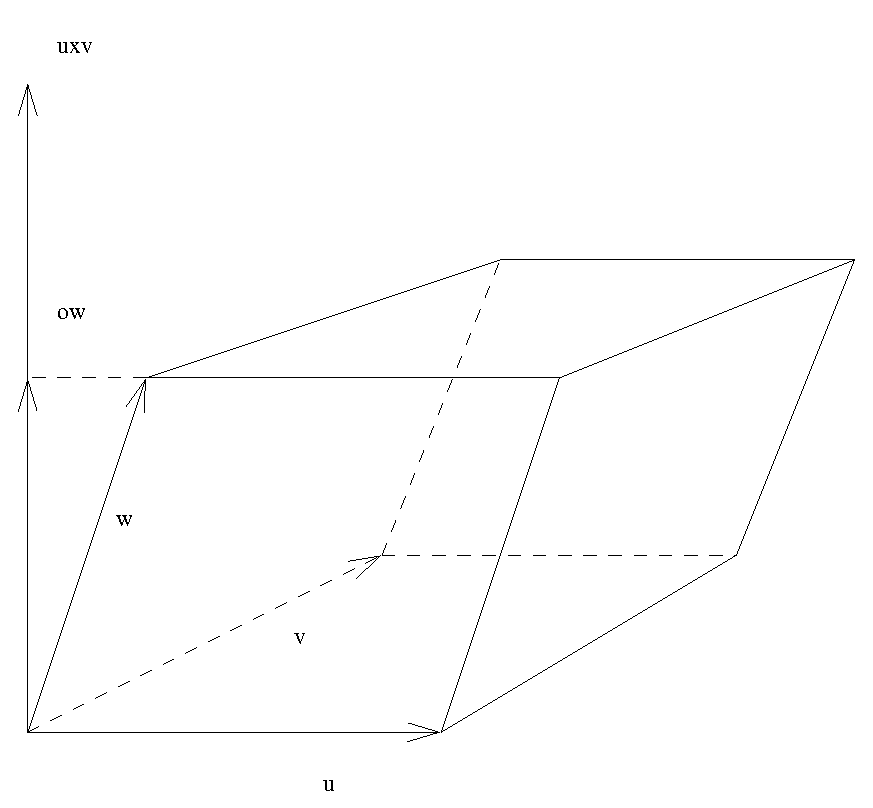
\includegraphics[height=1in]{../../modules/vectors/pictures/ok-volume_box.eps}

\column{0.75\textwidth}
\begin{itemize}
\item $A$, $B$, $C$, $D$ points in space;
\item<2-> $\textbf{u} = \textbf{AB}$, $\textbf{v}=\textbf{AC}$, $\textbf{w}=\textbf{AD}$;
\item<3-> $R=R(\textbf{u},\textbf{v},\textbf{w})$: box on sides $\textbf{u}$, $\textbf{v}$, $\textbf{w}$.\pause
\item<4-> $\text{Vol}(R) = |\textbf{u} \times \textbf{v}| |\textbf{r}| = |\textbf{u} \times \textbf{v}| \, |\textbf{proj}_{\bm{u} \times \bm{v}} \textbf{w}| =
|\textbf{w} \cdot (\textbf{u} \times \textbf{v})|\; .$
\end{itemize}
\end{columns}
\uncover<5->{
\begin{definition}
The quantity $\textbf{w} \cdot (\textbf{u} \times \textbf{v})$ is called the scalar triple product of $\fcv w, \fcv u, \fcv v$.
\end{definition}
}
\uncover<6->{
\begin{itemize}
\item If $\textbf{u} =\langle u_1,u_2,u_3\rangle$,
$\textbf{v} =\langle v_1,v_2,v_3\rangle$, and $\textbf{w} =\langle w_1,w_2,w_3\rangle$, then
%
$$\textbf{w} \cdot (\textbf{u} \times \textbf{v}) = \left|
\begin{array}{ccc}
w_1 & w_2 & w_3 \\
u_1 & u_2 & u_3 \\
v_1 & v_2 & v_3
\end{array}
 \right|$$
\end{itemize}
}
\end{frame}
\begin{frame}
  \frametitle{Orientations of Space}

\begin{itemize}
 \item The following are equivalent:
\begin{itemize}
  \item Every vector in space can be decomposed along $\textbf{u}$, $\textbf{v}$, $\textbf{w}$;
  \item The box $R(\textbf{u},\textbf{v},\textbf{w})$ is non-degenerate;
  \item $Vol(R(\textbf{u},\textbf{v},\textbf{w})) \neq 0$;
  \item $\textbf{u} \cdot (\textbf{v} \times \textbf{w}) \neq 0$.
\end{itemize}
%
\item \pause If any of the above is valid: $\{ \textbf{u}, \textbf{v}, \textbf{w}\}$ is a frame.

\item Rectangular coordinate system $\to$ fundamental frame $\{ \textbf{u}, \textbf{v}, \textbf{w}\}$

\item Consistent Right Hand Rule ($\textbf{w}=\textbf{u} \times \textbf{v}$) if and only if
%
$$\textbf{u} \cdot (\textbf{v} \times \textbf{w}) >0$$
%
The frame $\{ \textbf{u}, \textbf{v}, \textbf{w}\}$ is positively oriented if
$\textbf{u} \cdot (\textbf{v} \times \textbf{w}) >0$
%
\end{itemize}

\end{frame}
} %end lecture

% begin lecture
\lect{2014}{Lecture 4}{4}{
\begin{frame}
 \frametitle{Main Questions}


\begin{columns}[t]
\column[T]{0.4\textwidth}

\begin{pspicture}(-1,-2)(2,2)
\renewcommand{\fcScreen}{[-2 -1 -0.55] 0}
\tiny
\fcBoundingBox{-1}{-2}{2}{2}
\fcParallelogramIIId{[2 2 0]}{[1 2 -1]}{[1 2 2]}
\fcAxesIIId{2}{2}{2}
\fcLineIIId[arrows=->]{[ 0 0 0]}{[1 1 1]}
\fcDotIIId{[1 1 1]}
\fcPutIIId[lb]{[1 1 1]}{$~~Q(x,y,z)$}
\fcLineIIId{[0.6 0.95 0.35]}{[1.4 1.05 1.65]}

\fcLineIIId[arrows=->]{[ 0 0 0]}{[1 2 0.5]}
\fcDotIIId{[1 2 0.5]}
\fcPutIIId[lb]{[1 2 0.5]}{$~~P(x,y,z)$}
\end{pspicture}

\column{0.6\textwidth}
What condition(s) should
\begin{itemize}
\item the position vector
\item the coordinates
\end{itemize}

of a point satisfy for it to be on a specific

\begin{itemize}
\item line $L$
\item plane $\mathcal{P}$?
\end{itemize}
\end{columns}

Condition(s) in terms of:
\begin{itemize}
\item position vector $\Rightarrow$ vector (system of) equations;
\item coordinates $\Rightarrow$ scalar equations.
\end{itemize}
\end{frame}

\begin{frame}
\frametitle{Line from Point and Direction}
\begin{columns}
\column{0.3\textwidth}
\psset{xunit=1cm, yunit=1cm}
\begin{pspicture}(-0.2,-0.2)(3.5,2)
\tiny
\fcFullDot{0}{0}
\rput[tl](0,-0.1){$O$}
\psline(0, 1.7)(3.5,0.3)
\fcFullDot{0.5}{1.5}
\rput[bl](0.5, 1.5){$P_0$}
\uncover<4->{
\psline[arrows=->, linecolor=red](0.5,1.5)(2.5,0.7)
}
\psline[arrows=->, linecolor=blue](1,1.3)(2, 0.9)
\rput[b](1.5,1.2) {$\fcv u$}
\rput[l](3.5,0.3){$L$}

\uncover<2->{\psline[arrows=->](0,0)(0.5,1.5)
\rput[l](0.25, 0.75){$~~\fcv r_0$}
}
\uncover<3->{%
\psline[arrows=->](0,0)(2.5, 0.7)
\rput[b](2.5, 0.75){$P$}
\rput[t](1.25, 0.2){$\fcv r$}
}
\end{pspicture}

\column{0.7\textwidth}
\begin{itemize}
\item Suppose we have line $L$ that passes through point $P_0$ and has non-zero direction $\textbf{u}$.
\item<2-> Denote by $\fcv r_0=\fcv{OP}_0$ the position vector of $P_0$.
\item<3->$P$ with position vector $\textbf{r}$ is on $L$ $\Leftrightarrow$ 
\item<4->$\textbf{P}_0\textbf{P}$ has the same direction as $\textbf{u}$ $\Leftrightarrow$
\item<5-> $\textbf{P}_0\textbf{P}$ is a scalar multiple of $\textbf{u}$ $\Leftrightarrow$
\item<6-> $\textbf{r}-\textbf{r}_0 = t\textbf{u}$  for some real number $t$.
\end{itemize}
\end{columns}
\uncover<7->{
\begin{definition}
The equation 
\[
\fcv{r} = \fcv{r}_0+t\fcv{u}
\]
is called a parametric vectorial equation of the the line $L$.
\end{definition}
}
\end{frame}

\begin{frame}
\frametitle{Line from Point and Direction}
\begin{columns}
  \column{6cm}
\begin{itemize}
 \item Point $P_0(x_0,y_0,z_0)$, $\textbf{r}_0=\langle x_0,y_0,z_0\rangle$;
\item Direction $\textbf{u}=\langle u_1,u_2,u_3\rangle$.
\end{itemize}
  \column{5cm}
 $L$: line with direction $\textbf{u}$, \\passing through $P_0$
\end{columns}

\begin{columns}
  \column{6cm}
    \uncover<2->{$P$ with position vector $\textbf{r}$ is on $L$ $\leftrightarrow$ \\ }
    \uncover<3->{\medskip $\textbf{r} = \textbf{r}_0+t\textbf{u}$ $\leftrightarrow$\\}
    \uncover<4->{\medskip $\langle x,y,z\rangle = \langle x_0,y_0,z_0\rangle + t\langle u_1,u_2,u_3\rangle$ $\leftrightarrow$\\}
    \uncover<5->{\medskip \textcolor[rgb]{0.98,0.00,0.00}{Parametric scalar equations}:\\
    $\boxed{\left\{ \begin{array}{ll}
           x & = x_0 + t u_1 \\
	   y & = y_0 + t u_2 \\
           z & = z_0 + t u_3
          \end{array}
\right.}$  \\ for some real parameter $t$ }

  \column{6.5cm}
    \begin{figure}
        \psfrag{O}{$O$}
        \psfrag{x}{$x$}
        \psfrag{y}{$y$}
        \psfrag{z}{$z$}
        \psfrag{L}{$L$}
        \psfrag{P}{$P(x,y,z)$}
        \psfrag{P0}{$P_0(x_0,y_0,z_0)$}
        \psfrag{r}{$\textbf{r}$}
        \psfrag{u}{$\textbf{u}=\langle u_1,u_2,u_3\rangle$}
        \psfrag{r0}{$\textbf{r}_0$}
        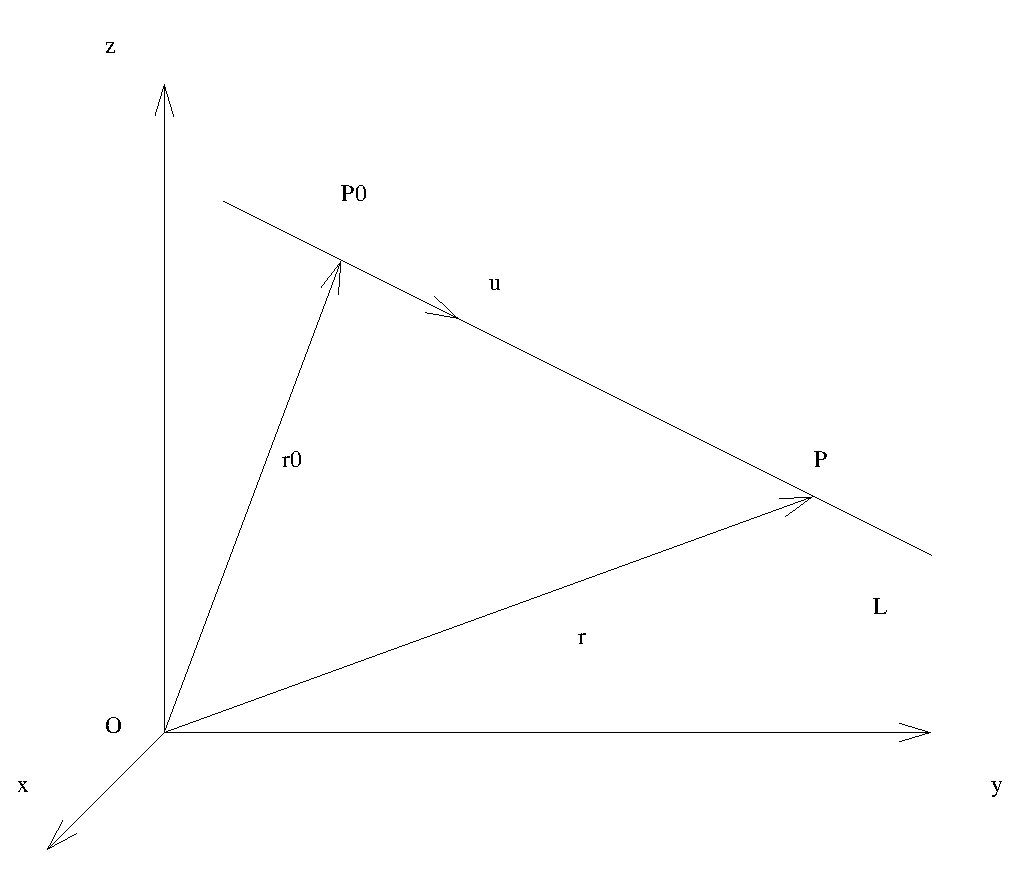
\includegraphics[height=2in]{../../modules/vectors/pictures/ok-line_point_direction_scalar.eps}
    \end{figure}
\end{columns}
\end{frame}

\begin{frame}
\uncover<1->{ $$\left\{ \begin{array}{ll}
           x & = x_0 + t u_1 \\
	   y & = y_0 + t u_2 \\
           z & = z_0 + t u_3
          \end{array}
\right. \Longrightarrow \boxed{\frac{x-x_0}{u_1} = \frac{y-y_0}{u_2} = \frac{z-z_0}{u_3}} \text{ \textcolor[rgb]{0.98,0.00,0.00}{Symmetric equations}}$$}

\uncover<2->{Caution! If $u_2=0$ (for example), then:
%
$$\frac{x-x_0}{u_1} = \frac{z-z_0}{u_3} \quad  \text{ and } \quad y=y_0 $$}

\uncover<3->{Example: Line with direction $\textbf{u} = \langle 4,5,6\rangle$ through $P_0(1,2,3)$:}
\begin{itemize}
 \item<4-> Parametric vectorial equation:
%
$$\textbf{r} = \langle 1,2,3\rangle + t \langle 4,5,6\rangle \leftrightarrow
\textbf{r} = \langle 1+4t, 2+5t, 3+6t\rangle$$
%
\item<5-> Parametric scalar equations:
%
$$\left\{ \begin{array}{ll}
           x & = 1 + 4t \\
	   y & = 2+5t \\
           z & = 3+6t
          \end{array}
\right. , \quad t \text{ real number.}$$
%
\item<6-> Symmetric equations:
%
$$\frac{x-1}{4} = \frac{y-2}{5} = \frac{z-3}{6}\; .$$
\end{itemize}

\end{frame}
\begin{frame}
 \frametitle{Line from Two Points}

\begin{columns}

\column{0.4\textwidth}
\psset{xunit=1.4cm, yunit=1.4cm}
\begin{pspicture}(-1,-0.4)(2,2.1)
\fcBoundingBox{-0.8}{-0.4}{4}{2.1}
\renewcommand{\fcScreen}{[-3 -1 -0.2] 0}
\tiny
\uncover<5->{\fcAxesIIId{2}{2}{2}}
\fcLineIIId{[0.5 0.5 1]}{[3 3 0.5]}
\fcLineIIId{[0.5 0.5 1]}{[4 4 0.3]}
\fcLineIIId[arrows=->]{[0 0 0]}{[1 1 0.9]}
\fcPutIIId[br]{[0.5 0.5 0.45]}{$\fcv r_0~$}

\fcLineIIId[linecolor=blue, arrows=->]{[1 1 0.9]}{[2.5 2.5 0.6]}
\fcPutIIId[br]{[1.75 1.75 0.8]}{$\fcv u$}

\fcLineIIId[arrows=->]{[0 0 0]}{[2.5 2.5 0.6]}
\fcPutIIId[b]{[1.25 1.25 0.3]}{$\fcv r_1$}

\fcDotIIId{[1 1 0.9]}
\fcPutIIId[lb]{[1 1 0.95]}{$P_0\uncover<5->{(x_0,y_0, z_0)} $}
\fcDotIIId{[2.5 2.5 0.6]}
\fcPutIIId[lb]{[2.5 2.5 0.65]}{$P_1\uncover<5->{(x_1, y_1, z_1)}$}
\fcDotIIId{[3.5 3.5 0.4]}
\fcLineIIId[arrows=->]{[0 0 0]}{[3.5 3.5 0.4]}
\fcPutIIId[b]{[1.75 1.75 0.2]}{$\fcv r$}
\fcPutIIId[b]{[3.5 3.5 0.5]}{$~P(x,y,z)$}
\fcPutIIId[t]{[4 4 0.3]}{$~L$}
\fcPutIIId[r]{[0 0 0.1]}{$O~~$}
\end{pspicture}
\column{0.6\textwidth}
\begin{itemize}
\item Given: distinct points $P_0$ and $P_1$, position vectors $\textbf{r}_0$ and $\textbf{r}_1$.
\item Goal: write equations of line $L$ through $P_0$ and $P_1$.
\item<2-> Direction of $L$: $\textbf{u} = \textbf{r}_1 - \textbf{r}_0$.
\item<5-> $\fcv{u} = \langle x_1-x_0,y_1-y_0,z_1-z_0\rangle$
\end{itemize}. 
\end{columns}
\uncover<3->{
\begin{definition}
\alert<1->{Parametric vectorial equation} of a line $L$:\\
$
\textbf{r} = \textbf{r}_0 + t(\textbf{r}_1-\textbf{r}_0)
\quad \Leftrightarrow \quad   \textbf{r} = (1-t)\textbf{r}_0 + t\textbf{r}_1
$

\uncover<5->{
\alert<1->{Parametric scalar equations} of a line $L$:
$\left|
\begin{array}{ll}
x & = x_0 + t(x_1-x_0) \\
y & = y_0 + t(y_1-y_0) \\
z & = z_0 + t(z_1-z_0)
\end{array}
\right. \Leftrightarrow \left| \begin{array}{ll}
x & = (1-t)x_0 + tx_1 \\
y & = (1-t)y_0 + ty_1 \\
z & = (1-t)z_0 + tz_1
\end{array}
\right. , \quad t \text{ real number.}$
} %uncover
\end{definition}
} %uncover
\end{frame}
\begin{frame}
\frametitle{Plane from Point and Normal}
\begin{columns}
\column{0.3\textwidth}
\psset{xunit=1cm, yunit=1cm}
\begin{pspicture}(-0.2, -0.2)( 2,2)
\tiny%
\renewcommand{\fcScreen}{[-1.5 2 -0.5 ] 0}%
\fcParallelogramIIId{[-0.1 -0.1 1]}{[1.6 -0.1 -0.7]}{[0 2 3]}%
\fcLineIIId[arrows=->]{[1 1 1]}{[2 0 2]}%
\fcPutIIId[l]{[1.5 0.5 1.5]}{$~~\fcv n\uncover<5->{\langle a,b,c\rangle}$}%
\uncover<3->{%
\fcPerpendicularIIId{[2 0 2]}{ [1 1 1] [0.2 0.4 1.2]}{0.4}%
}%
\fcDotIIId{[1 1 1]}%
\fcPutIIId[lt]{[1 1 1]}{$P_0\uncover<6->{(x_0, y_0, z_0)}$}%
\uncover<2->{%
\fcDotIIId{[0.2 0.4 1.2]}%
\fcPutIIId[bl]{[0.2 0.4 1.2]}{$P\uncover<6->{(x,y,z)}$}%
}%
\uncover<3->{%
\fcLineIIId[arrows=->]{[1 1 1]}{[0.2 0.4 1.2]}%
}%
\fcLineIIId[arrows=->]{[0 0 0]}{[1 1 1]}%
\fcPutIIId[tl]{[0.5 0.5 0.5]}{$~\fcv r_0$}%
\uncover<2->{%
\fcLineIIId[arrows=->]{[0 0 0]}{[0.2 0.4 1.2]}%
}%
\fcPutIIId[r]{[0.1 0.2 0.6]}{$\fcv r~$}%
\fcAxesIIId{2}{2}{2}%
\end{pspicture}
\column{0.7\textwidth}
\begin{itemize}
\item<1-> Point $P_0$, with position vector $ \fcv{r}_0$;
\uncover<5->{$ \fcv{r}_0 = \langle x_0,y_0,z_0\rangle$}
\item<1-> Direction $ \fcv{n}$, non-zero vector.
\uncover<5->{$ \fcv{n} = \langle a,b,c\rangle$}
\item<1->Goal: describe plane passing through $P_0$ and orthogonal to $\fcv n$.
\item<2-> Point $P$ with position $ \fcv{r}$ is on $\mathcal{P}$ $\Leftrightarrow$
\item<3->{$ \alert<4>{\fcv{P}_0 \fcv{P}\uncover<4->{=\fcv r-\fcv r_0}} $ is orthogonal (normal) to $ \fcv{n}$ $\Leftrightarrow$}
\item<5->{\alert<5->{Implicit vectorial equation}: $ (\alert<8>{ \fcv{r}- \fcv{r}_0}) \cdot  \alert<9>{\fcv{n}} = 0.$}
\item<6->{A point $P(x,y,z)$ is on $\mathcal{P}$ $\Leftrightarrow$}

\end{itemize}
\end{columns}
\uncover<7->{%
\begin{definition}[\alert<7->{Implicit scalar equation}]
$\alert<8>{ \langle x-x_0, y-y_0, z-z_0\rangle} \cdot \alert<9>{\langle a,b,c\rangle} = 0$ \uncover<10->{$\Leftrightarrow$} 
\uncover<10->{\alert<10>{$a(x-x_0) + b(y-y_0)+c(z-z_0) = 0$}}
\end{definition}
} %uncover
\end{frame}
Find an equation of plane $\mathcal P$ passing through the point and parallel to the given directions.

\begin{enumerate}
\item $P_0(1,2,3)$, $\fcv u=(2,3,5)$, $\fcv v=(3,5,7 )$.

\answer{$\mathcal P: z+y-4 x-1 =0$}
\item $P_0(1,1,1)$, $\fcv u=(1,-1,0)$, $\fcv v= (0,1,-1)$.
\answer{$\mathcal P:  z+y+x-3  =0$}
\end{enumerate}

\begin{frame}
 \frametitle{Plane from Three Points}

\begin{columns}
\column{0.4\textwidth}
\psset{xunit=0.8cm, yunit=0.8cm}
\begin{pspicture}(-0.2, -0.2)(3,3)
\tiny
\renewcommand{\fcScreen}{[-2 -1 -0.5] 0}
\fcParallelogramIIId{[-0.8 -0.8 3.6]}{[-1.4 2.4 1]}{[2.4 -1.4 1]}
\fcPutIIId[l]{[0 0 0.05]}{$~~O$}
\fcDotIIId{[0 0 0]}

\fcLineIIId[arrows=->, linestyle=dotted]{[0 0 0]}{[2 0 0]}
%\fcPutIIId{[1 0 0]}{$\fcv r_2$}
\fcLineIIId[arrows=->, linestyle=dotted]{[0 0 0]}{[0 2 0]}
%\fcPutIIId{[0 1 0]}{$\fcv r_0$}
\fcLineIIId[arrows=->, linestyle=dotted]{[0 0 0]}{[0 -0.4 2.4]}
%\fcPutIIId{[0 -0.2 1.2]}{$\fcv r_1$}
\fcDotIIId{[2 0 0]}
\fcDotIIId{[0 2 0]}
\fcDotIIId{[0 -0.4 2.4]}
\fcPutIIId[r]{[2 0 0]}{ $P_2(\fcv r_2)~$}
\fcPutIIId[tl]{[0 2 0]}{ $P_0(\fcv r_0)$}
\fcPutIIId[b]{[0 -0.4 2.4]}{ $P_1(\fcv r_1)$}
\fcLineIIId[arrows=->]{[0 2 0]}{[2 0 0]}
\fcPutIIId[t]{[1 1 -0.1]}{$~\fcv v$}
\fcLineIIId[arrows=->]{[0 2 0]}{[0 -0.4 2.4]}
\fcPutIIId[b]{[0 0.8 1.3]}{$~\fcv u$}%
\fcPerpendicularIIId{[4.8 6.8 4.8]}{ [0 2 0] [2 0 0]}{0.6}%
\fcPerpendicularIIId[arrows=<-]{[4.8 6.8 4.8]}{[0 2 0] [0 -0.4 2.4]}{0.6}%
\fcLineIIId[linestyle=dotted]{[0 0 0]}{[1.4 -0.84 1.44]}%
\fcPerpendicularIIId[arrows=<-]{[4.8 6.8 4.8]}{[0 2 0] [1.4 -0.84 1.44]}{0.8}%
\fcLineIIId[arrows=->]{[0 2 0]}{[1.4 -0.84 1.44]}%
\fcPutIIId[b]{[1.4 -0.84 1.44]}{$P(\fcv r)$}%
\end{pspicture}

\column{0.6\textwidth}
\begin{itemize}
\item Given: three non-collinear points $P_0(\fcv{r}_0)$, $P_1(\fcv{r}_1)$, $P_2(\fcv{r}_2)$.
\item Goal: find equations fo plane $\mathcal{P}$ passing through $P_0$, $P_1$, and $P_2$.
\item<2-> The plane is parallel to $\fcv{u} = \fcv{P}_0\fcv{P}_1 = \fcv{r}_1 -\fcv{r}_0$ and passing through $P_0$ $\Rightarrow$ this problem was solved previously.

\end{itemize}
\end{columns}
\only<3>{
Normal $\fcv{n} = \fcv{u} \times \fcv{v} =
(\fcv{r}_1-\fcv{r}_0) \times (\fcv{r}_2-\fcv{r}_0)$  \\

\alert<1->{Implicit equation}:
$$(\fcv{r}-\fcv{r}_0) \cdot \fcv{n} = 0$$
$$\boxed{(\fcv{r}-\fcv{r}_0) \cdot [(\fcv{r}_1-\fcv{r}_0) \times (\fcv{r}_2-\fcv{r}_0)] = 0}$$
$$\text{Vol}(R(\fcv{P}_0\fcv{P}, \fcv{P}_0\fcv{P}_1, \fcv{P}_0\fcv{P}_2)) = 0$$
}

\only<4>{
\alert<1->{Implicit equation}: $(\fcv{r}-\fcv{r}_0) \cdot [(\fcv{r}_1-\fcv{r}_0) \times (\fcv{r}_2-\fcv{r}_0)] = 0$

Let the points have coordinates $P_0(x_0,y_0,z_0)$, $P_1(x_1,y_1,z_1)$, $P_2(x_2,y_2,z_2)$. $P(x,y,z)$ is on plane $\mathcal{P}$:

\alert<1->{Implicit scalar equation}:
$\left| \begin{array}{ccc}
x-x_0 & y-y_0 & z-z_0 \\
x_1-x_0 & y_1-y_0 & z_1-z_0 \\
x_2-x_0 & y_2-y_0 & z_2-z_0
\end{array}
\right| = 0\; .$
}

\vskip 10cm
\end{frame}


\begin{frame}
\frametitle{Relationships betwee points lines and planes}

\begin{itemize}
\item So far we studied the following geometric objects/
\begin{itemize}
\item Points: $P(\textbf{r})$.
\item Lines: $L$: $\textbf{r}= \textbf{r}_0 + t\textbf{u}$
\item Planes: $\mathcal{P}$: $(\textbf{r}-\textbf{r}_0)\cdot \textbf{n} =0$
\end{itemize}
\item We investigate the following relationships/geometric quantities:
\begin{itemize}
\item Parallelism
\item Perpendicularity
\item Angles
\item Distances
\item Intersections
\end{itemize}
\end{itemize}
\end{frame}
\begin{frame}
  \frametitle{Point and line}
  Point $P(\textbf{r}_1)$ \hspace{2cm} Line $L: \quad \textbf{r}=\textbf{r}_0+t\textbf{u}$

  \begin{columns}
  \column{6cm}
  \textcolor[rgb]{0.98,0.00,0.00}{Distance} from $P$ to $L$:
  \uncover<2->{
  $$d(P,L) = |\textbf{\text{orth}}_{\bm{u}}(\textbf{r}_1-\textbf{r}_0)|$$
  $$\boxed{d(P,L) = \frac{|(\textbf{r}_1-\textbf{r}_0) \times \textbf{u}|}{|\textbf{u}|}}$$}
  %
  \column{6.5cm}
      \begin{figure}
        \psfrag{L}{$L$}
        \psfrag{P}{$P(\textbf{r}_1)$}
        \psfrag{P0}{$P_0(\textbf{r}_0)$}
        \psfrag{u}{$\textbf{u}$}
        \psfrag{r12}{$\textbf{r}_1-\textbf{r}_0$}
        \psfrag{orth}{$\textbf{\text{orth}}_{\bm{u}}(\textbf{r}_1-\textbf{r}_0)$}
        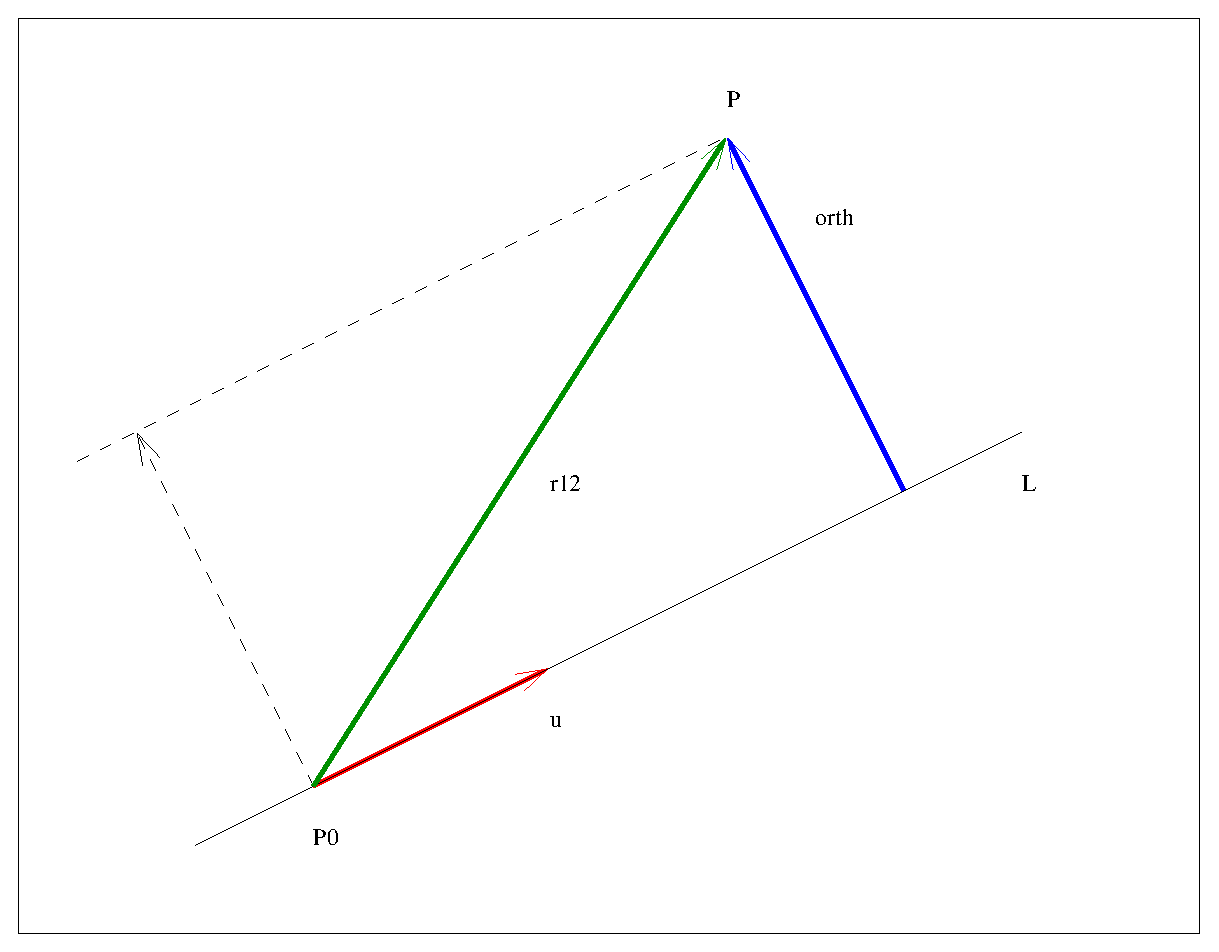
\includegraphics[height=2in]{../../modules/vectors/pictures/ok-distance_point_line.eps}
    \end{figure}
    \end{columns}
\end{frame}
\begin{frame}
  \frametitle{Distance between point and plane}
  \begin{columns}
  
  \column{0.4\textwidth}
          \psfrag{cP}{$\mathcal{P}$}
          \psfrag{P}{$P(\textbf{r}_1)$}
          \psfrag{P0}{$P_0(\textbf{r}_0)$}
          \psfrag{n}{$\textbf{n}$}
          \psfrag{r12}{$\textbf{r}_1\!-\!\textbf{r}_0$}
          \psfrag{proj}{$\textbf{\text{proj}}_{\bm{n}}(\textbf{r}_1\!-\!\textbf{r}_0)$}
          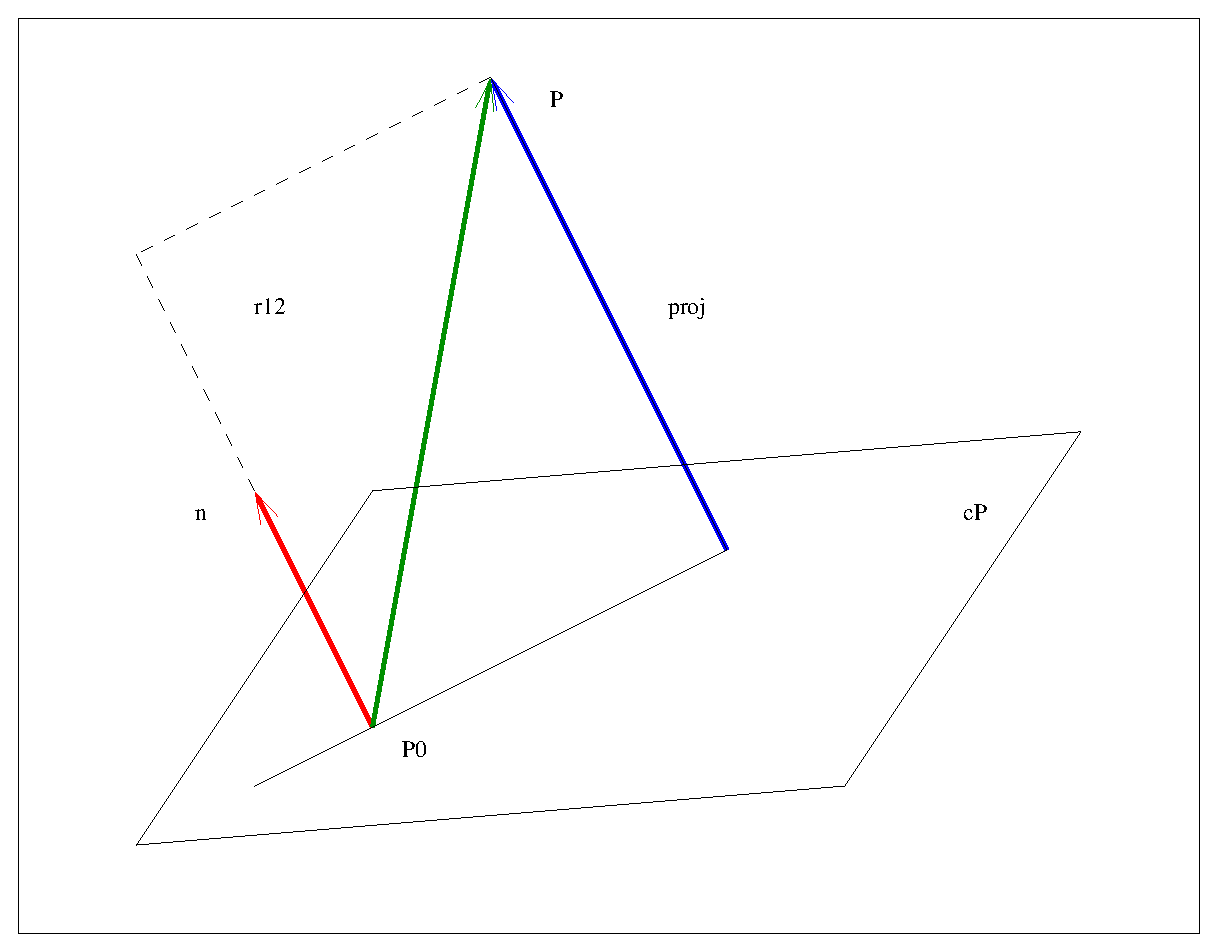
\includegraphics[height=1.3in]{../../modules/vectors/pictures/ok-distance_point_plane.eps}
\column{0.6\textwidth}
\begin{itemize}
\item Given: point $P(\textbf{r}_1)$,
\item plane $\mathcal{P}: \quad (\textbf{r}-\textbf{r}_0)\cdot \textbf{n} = 0$.
\item Goal: find the distance between $P$ and $\mathcal P$. 
\end{itemize}
\alert<1->{Distance} from $P$ to $\mathcal{P}$:
\uncover<2->{
$$d(P,\mathcal{P}) = |\textbf{\text{proj}}_{\bm{n}}(\textbf{r}_1-\textbf{r}_0)|$$
$$d(P,\mathcal{P}) = \frac{|(\textbf{r}_1-\textbf{r}_0) \cdot \textbf{n}|}{|\textbf{n}|}$$}

\uncover<3->{\alert<1->{Scalar equation}:
$P(x_1,y_1,z_1)$
$$\mathcal{P}: ax+by+cz+d=0$$}
\uncover<4->{$$\textbf{n} = \langle a,b,c\rangle$$
$$\boxed{\text{Distance} = \frac{|ax_1+by_1+cz_1+d|}{\sqrt{a^2+b^2+c^2}}}$$}
\end{columns}
\end{frame}
\begin{frame}
  \frametitle{Parallel lines}
    Lines
    $$L_1: \quad \textbf{r}= \textbf{r}_1+t\textbf{u}_1 \qquad L_2: \quad \textbf{r}= \textbf{r}_2+s\textbf{u}_2$$
\begin{columns}[t]
  \column[T]{6cm}
  \textcolor[rgb]{0.98,0.00,0.00}{Parallel} lines\\
    %\medskip
    \uncover<2->{
    $L_1 || L_2$ $\Longleftrightarrow$
    $\textbf{u}_1$, $\textbf{u}_2$ collinear $\Longleftrightarrow$
    $$\boxed{\textbf{u}_1 \times \textbf{u}_2 = \textbf{0}}$$}
    \uncover<3->{
    \textcolor[rgb]{0.98,0.00,0.00}{Distance}:
    $$d= d(L_1,L_2)  = d(P_1,L_2) = d(P_2,L_1)$$}
    \uncover<4->{
    $$d= d(L_1,L_2) = |\textbf{\text{orth}}_{\bm{u}_1} (\textbf{r}_2-\textbf{r}_1)|$$
    $$\boxed{d = \frac{|(\textbf{r}_2-\textbf{r}_1) \times \textbf{u}_1|}{|\textbf{u}_1|} =\frac{|(\textbf{r}_2-\textbf{r}_1) \times \textbf{u}_2|}{|\textbf{u}_2|}}$$}
    %\textcolor[rgb]{0.98,0.00,0.00}{Identical} lines: $d(L_1,L_2)=0$
    %$$\textbf{u}_1\times \textbf{u}_2 = \textbf{0} \text{ and }
    %(\textbf{r}_2-\textbf{r}_1) \times \textbf{u}_1 = \textbf{0}$$
  \column{6.5cm}
  \begin{figure}
        \psfrag{L1}{$L_1$}
        \psfrag{L2}{$L_2$}
        \psfrag{P1}{$P_1$}
        \psfrag{P2}{$P_2$}
        \psfrag{r21}{$\textbf{r}_2-\textbf{r}_1$}
        \psfrag{u1}{$\textbf{u}_1$}
        \psfrag{u2}{$\textbf{u}_2$}
        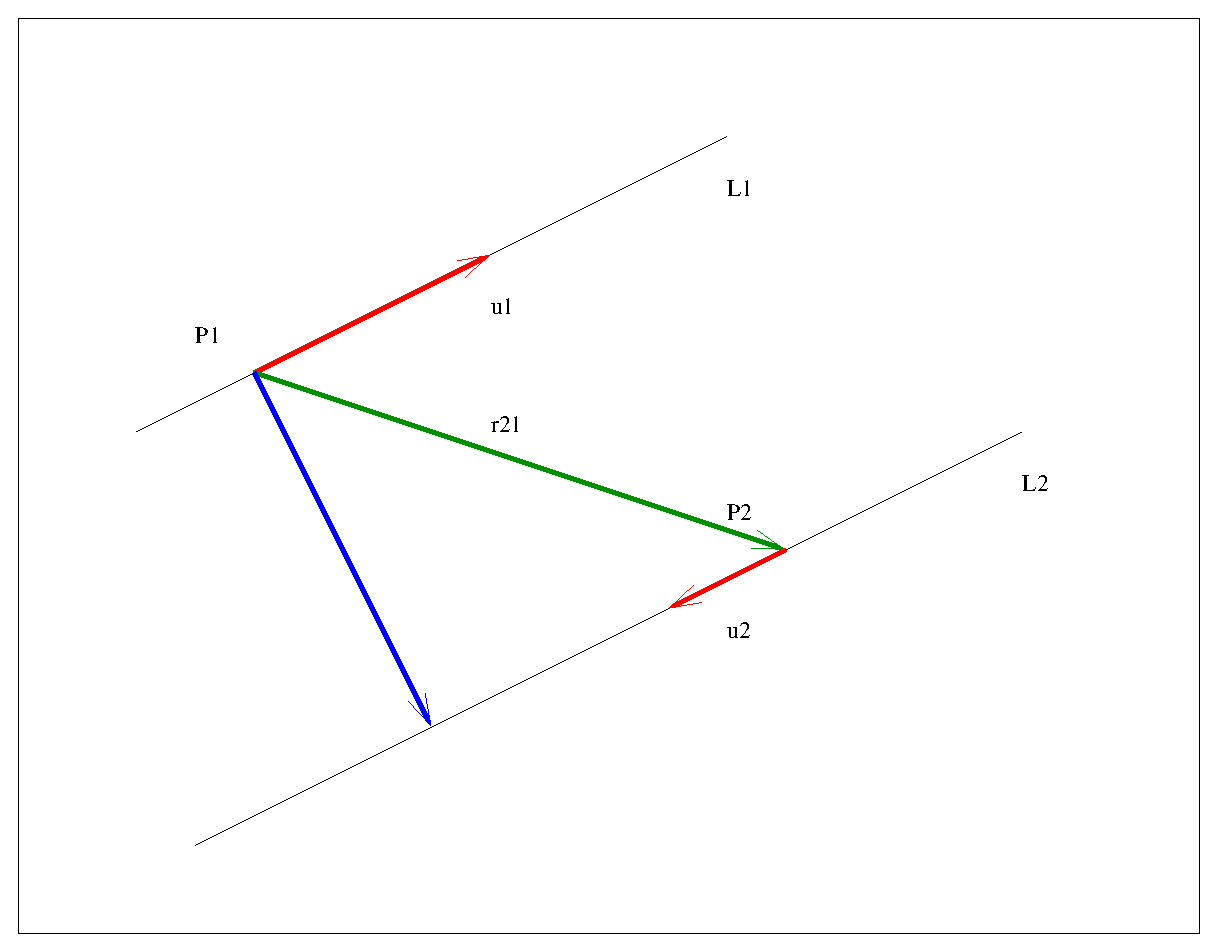
\includegraphics[height=2in]{../../modules/vectors/pictures/ok-distance_parallel_lines.eps}
    \end{figure}
\end{columns}

\end{frame}
\begin{frame}
\frametitle{Angle between lines}

\begin{columns}
\column{0.4\textwidth}
\begin{pspicture}(-2, -2)(2,2)
\tiny
\renewcommand{\fcScreen}{[-1 0 -0.5] 0}
\fcParallelogramIIId{[1.2 -1.2 1]}{[1.2 1.2 1]}{[-1.2 -1.2 1]}
\fcLineIIId{[-1 -1 -1]}{[1 1 -1]}
\fcLineIIId{[1 -1 1]}{[-1 1 1]} 
%\fcPerpendicularIIId[arrows=->, linecolor=green]{[0 0 -1]}{[1 -1 1] [-1 1 1]}{0.2}
\fcLineIIId[arrows=->, linecolor=blue]{[0 0 -1]}{[0 0 1]}
\fcLineIIId[linestyle=dotted]{[-1 -1 1]}{[1 1 1]}
\fcLineIIId[linecolor=red, arrows=->]{[0 0 -1]}{[0.75 0.75 -1]}
\fcPutIIId[t]{[0.325 0.325 -1.1]}{$\fcv u_1$}
\fcDotIIId{[0 0 -1]}
\fcPutIIId[r]{[-0.1 0.1 -1]}{$P_1$}


\fcDotIIId{[0 0 1]}
\fcPutIIId[r]{[-0.1 0.1 1]}{$P_2$}

\fcLineIIId[linecolor=red, arrows=->]{[0 0 1]}{[-0.75 0.75 1]}
\fcPutIIId[br]{[-0.325 0.325 1]}{$\fcv u_2$}

\fcLineIIId[linecolor=red, arrows=->]{[0 0 1]}{[0.75 0.75 1]}
\fcPutIIId[t]{[0.325 0.325 0.9]}{$\fcv u_1$}
\fcPutIIId[linecolor=brown]{[0 0 1]}{\fcAngleIIId{[0.5 0.5 0]}{[-0.5 0.5 0]}{0.2}}

\fcPutIIId{[2 2 0]}{%
\fcLineIIId[linecolor=red, arrows=->]{[0 0 1]}{[-0.75 0.75 1]}
\fcPutIIId[br]{[-0.325 0.325 1]}{$\fcv u_2$}
\fcLineIIId[linecolor=red, arrows=->]{[0 0 1]}{[0.75 0.75 1]}
\fcPutIIId[t]{[0.325 0.325 0.9]}{$\fcv u_1$}
\fcPutIIId[linecolor=brown]{[0 0 1]}{
\fcAngleIIId{[0.5 0.5 0]}{[-0.5 0.5 0]}{0.3}
\fcPutIIId[l]{[0 0.35 0]}{$\alpha$}
}
}%
\end{pspicture}

\psfrag{L1}{$L_1$}
\psfrag{L2}{$L_2$}
\psfrag{P1}{$P_1$}
\psfrag{P2}{$P_2$}
\psfrag{u1}{$\textbf{u}_1$}
\psfrag{u2}{$\textbf{u}_2$}
\psfrag{a}{$\alpha$}
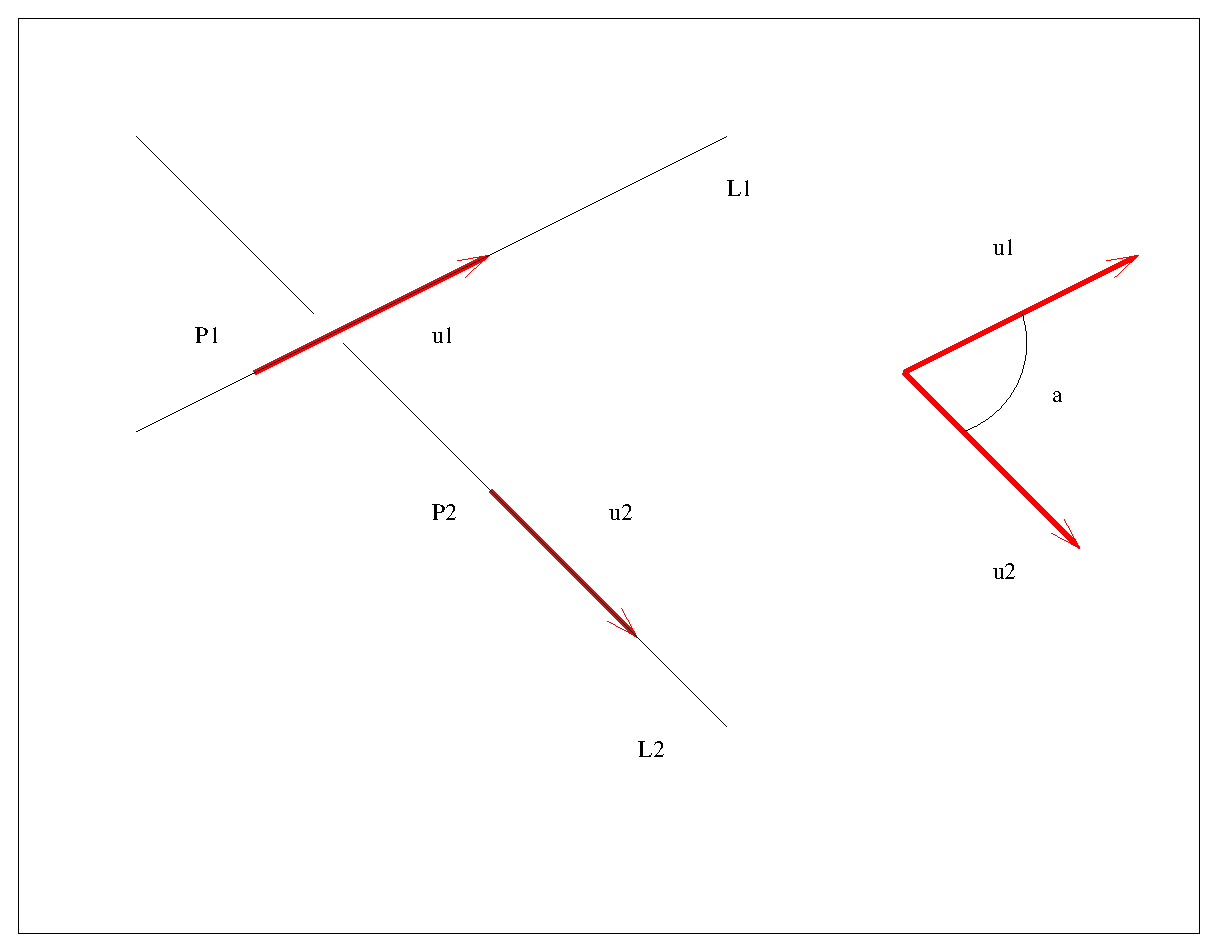
\includegraphics[height=1.4in]{../../modules/vectors/pictures/ok-angle_line_line.eps}
\column{0.6\textwidth}
\begin{itemize}
\item Given: lines $ \begin{array}{rrcl}L_1:&  \textbf{r}&=& \textbf{r}_1+t\textbf{u}_1 \\ L_2:& \textbf{r}&=& \textbf{r}_2+s\textbf{u}_2\end{array}$.
\item Goal: find angle between $L_1$ and $L_2$.
\end{itemize}
\alert<1->{Perpendicular} lines
\uncover<2->{
$L_1 \bot L_2$ $\Longleftrightarrow$
$\textbf{u}_1 \bot \textbf{u}_2$ $\Longleftrightarrow$
$$\boxed{\textbf{u}_1 \cdot \textbf{u}_2 = 0}$$}
\uncover<3->{
\alert<1->{Angle} between lines}
\uncover<4->{
$\alpha$: angle between $L_1$, $L_2$ $\Longleftrightarrow$ 
$\alpha$: acute angle $\textbf{u}_1$, $\textbf{u}_2$}
\uncover<5->{$\Longleftrightarrow$
$$\boxed{\alpha = \arccos\left( \frac{|\textbf{u}_1 \cdot \textbf{u}_2|}{|\textbf{u}_1| \, |\textbf{u}_2|}\right) }$$}
\end{columns}
\end{frame}
\begin{frame}
\frametitle{Distance between non-parallel lines}
\begin{columns}
\column{0.4\textwidth}
\begin{pspicture}(-2, -2)(2,2)
\tiny
\renewcommand{\fcScreen}{[-1 0 -0.5] 0}
\fcBoundingBox{-2}{-2}{2}{2}
\uncover<2->{%
\fcParallelogramIIId{[1.2 -1.2 1]}{[1.2 1.2 1]}{[-1.2 -1.2 1]}
\fcPutIIId[b]{[-1.2 -1.2 1]}{$\mathcal P$}
}%
\fcLineIIId{[-1 -1 -1]}{[1 1 -1]}
\fcLineIIId{[1 -1 1]}{[-1 1 1]} 
%\fcPerpendicularIIId[arrows=->, linecolor=green]{[0 0 -1]}{[1 -1 1] [-1 1 1]}{0.2}
\fcPutIIId[l]{[-1 1 1]}{$~~L_1$}
\fcPutIIId[r]{[-1 -1 -1.2]}{$L_2$}
\uncover<6->{%
\fcLineIIId[linestyle=dotted]{[0 0 1.3]}{[0 0 -1.3]}%
\fcPutIIId[rt]{[-0.1 0.1 -1]}{$Q_2~~~$}%
}%
\uncover<10->{%
\fcPerpendicularIIId[linestyle=none]{[0 0 -0.125]}{[0 0 1] [1 1 1]}{0.2}%
\fcPerpendicularIIId[linestyle=none]{[0 0 -0.125]}{[0 0 1] [-1 1 1]}{0.2}%
}%
\uncover<13->{%
\fcLineIIId[arrows=->, linecolor=green]{[0.8 -0.8 1]}{[0.9 0.9 -1]}%
\fcLineIIId[arrows=->, linecolor=green]{[0 0 1]}{[0.1 1.7 -1]}%
\fcDotIIId{[0.1 1.7 -1]}%
\fcPutIIId[l]{[0.1 1.7 -1]}{$~~R$}%
\fcPutIIId[l]{[0.05 0.85 0]}{$\fcv r_2- \fcv r_1$}%
}%
\uncover<6->{%
\fcPerpendicularIIId{[0.8 0.8 -1]}{[0 0 -1]}{0.2}
}%
\uncover<14->{\fcLineIIId[arrows=->, linecolor=brown]{[0.8 -0.8 1]}{[0 0 1]}%
\fcLineIIId[arrows=->, linecolor=brown]{[0.9 0.9 -1]}{[0.1 1.7 -1]}%
}%
\uncover<15->{%
\fcPerpendicularIIId{[0.1 1.7 -1]}{[0 0 -1]}{0.2}%
}%
\uncover<11->{%
\fcLineIIId[arrows=->, linecolor=blue]{[0 0 1]}{[0 0 -0.125]}%
\fcPutIIId[r]{[0 0 0.4375]}{$\fcv n~$}
}%
\uncover<4->{%
\fcLineIIId[linestyle=dotted]{[-1 -1 1]}{[1 1 1]}
\fcPutIIId[l]{[1 1 1]}{$~~L_2'$}
}%
\fcLineIIId[linecolor=red, arrows=->]{[0 0 -1]}{[0.75 0.75 -1]}
\fcPutIIId[t]{[0.325 0.325 -1.1]}{$\fcv u_2$}
\fcDotIIId{[0 0 -1]}
\uncover<12->{%
\fcDotIIId{[0.8 -0.8 1]}%
\fcPutIIId[br]{[0.8 -0.8 1]}{$P_1~$}%
\fcDotIIId{[0.9 0.9 -1]}%
\fcPutIIId[tr]{[0.9 0.9 -1]}{$P_2~$}%
}%
\uncover<5->{%
\fcDotIIId{[0 0 1]}
\fcPutIIId[r]{[-0.1 0.1 1]}{$Q_1~~~$}
}%
\fcLineIIId[linecolor=red, arrows=->]{[0 0 1]}{[-0.75 0.75 1]}
\fcPutIIId[br]{[-0.325 0.325 1]}{$\fcv u_1$}
\uncover<2->{
\fcLineIIId[linecolor=red, arrows=->]{[0 0 1]}{[0.75 0.75 1]}
\fcPutIIId[t]{[0.325 0.325 0.9]}{$\fcv u_2$}
}
%\fcPutIIId{[2 2 0]}{%
%\fcLineIIId[linecolor=red, arrows=->]{[0 0 1]}{[-0.75 0.75 1]}
%\fcPutIIId[br]{[-0.325 0.325 1]}{$\fcv u_1$}
%\fcLineIIId[linecolor=red, arrows=->]{[0 0 1]}{[0.75 0.75 1]}
%\fcPutIIId[t]{[0.325 0.325 0.9]}{$\fcv u_2$}
%}%
\end{pspicture}

\column{0.6\textwidth}
\begin{itemize}
\item Given: lines $\begin{array}{rrcl}L_1: & \fcv{r}&=& \fcv{r}_1+t\fcv{u}_1 \\ L_2:& \fcv{r} &=& \fcv{r}_2+s\fcv{u}_2\end{array}$
\item The lines are skew or intersecting, i.e., $\fcv{n} = \fcv{u}_1 \times \fcv{u}_2 \neq \fcv{0}$.
\item Goal: find distance between the lines = $d(L_1, L_2)$ = shortest distance b-n points on the two lines.
\end{itemize}
\end{columns}
\begin{itemize} 
\only<handout:1|1-8>{
\item<2-> Construct plane $\mathcal P$ with directions $\fcv u_1$, $\fcv u_2$ and passing through $L_1$. 
\item<3-> Distance b-n $L_2$ and points on $\mathcal P$ is constant.
\item<4-> Project $L_2$ orthogonally on $\mathcal P$; let the projection be $L_2'$.
\item<5-> Let $L_2' $ and $L_1$ intersect in point $Q_1$.
\item<6-> Let $Q_2$ be the heel of the perpendicular from $Q_1$ onto $Q_2$.
\item<7-> $\Rightarrow$ $Q_1Q_2=d(L_1, L_2)$.
}
\only<handout:1|8-16>{
\item \alert<8,9>{$|Q_1Q_2|=d(L_1, L_2)$}.
}
\only<handout:2|9-16>{
\item<10-> $\fcv Q_1\fcv Q_2 \perp L_1, L_2$ \uncover<11->{$\Rightarrow$  $\fcv Q_1 \fcv Q_2$ is proportional to $\fcv n = \fcv u_1\times \fcv u_2$.}
\item<12-> Pick arbitrary points on $L_1, L_2$ - say, the base points $P_1(\fcv r_1), P_2(\fcv r_2)$.
\item<13-> Let $R$ be such that $\fcv Q_1\fcv R=\fcv P_1 \fcv P_2=\fcv r_2-\fcv r_1$. 
\item<14-> Then $\fcv{P}_2\fcv R$ is proportional to $\fcv u_1$.
\item<15-> $\Rightarrow $ $\fcv Q_2\fcv R= \fcv Q_2  \fcv P_2+\fcv{P}_2\fcv{R}$ is perpendicular to $\fcv n$.
}
\only<handout:3|16->{
\item<16->\alert<16,17>{ $\Rightarrow$ $\fcv Q_1 \fcv Q_2= \fcv {proj} _{\fcv n} (\fcv r_2-\fcv r_1)$.}
}
\only<handout:3|17->{
\item<18-> 
$d(L_1,L_2)  = |\fcv{proj}_{\alert<19>{\fcv{n}}} (\fcv{r}_2-\fcv{r}_1)| \uncover<19->{= \boxed{\frac{|(\fcv{r}_2-\fcv{r}_1)\cdot \alert<19,20>{\fcv{n}} | }{ |\alert<19,20>{\fcv{n}}|}}} \uncover<20->{= \frac{ |(\fcv{r}_2 -\fcv{r}_1 )\cdot (\alert<20>{ \fcv{u}_1\times \fcv{u}_2})|}{ | \alert<20>{\fcv{u}_1\times \fcv{u}_2}|}}$
\item<21-> If lines are intersecting we know $d(L_1,L_2)=0$. \uncover<22->{Since the lines intersect $L_2$ and $L_2'$ coincide.} \uncover<23->{$\Rightarrow$ $(\fcv{r}_2-\fcv{r}_1) \cdot (\fcv{u}_1\times \fcv{u}_2) = 0$} \uncover<24->{$\Rightarrow $ the formula $d(L_1, L_2)= \frac{|(\fcv{r}_2 - \fcv{r}_1 )\cdot (\fcv{u}_1\times \fcv{u}_2)|}{ | \fcv{u}_1\times \fcv{u}_2|}=0$ produces the expected result.}
}
\end{itemize}

\vskip 5cm
\end{frame}


\begin{frame}
  \frametitle{Parallel line and plane}
     Line $L: \quad \textbf{r}= \textbf{r}_1+t\textbf{u}$\hspace{2cm}
     Plane $\mathcal{P}: \quad (\textbf{r}-\textbf{r}_0) \cdot \textbf{n} = 0$
\bigskip
  \begin{columns}[t]
    \column{6cm}
    Line \textcolor[rgb]{0.98,0.00,0.00}{parallel} to plane\\
    \uncover<2->{
    $L || \mathcal{P}$ $\Longleftrightarrow$
    $\textbf{u} \bot \textbf{n}$ $\Longleftrightarrow$
    $$\boxed{\textbf{u} \cdot \textbf{n} = 0}$$}
    \uncover<3->{
    \textcolor[rgb]{0.98,0.00,0.00}{Distance} from $L$ to $\mathcal{P}$:
    $$d(L,\mathcal{P}) = d(P_1,\mathcal{P})$$}
    \uncover<4->{
    $$d=|\textbf{\text{orth}}_{\bm{u}}(\textbf{r}_1-\textbf{r}_0)| =
    |\textbf{\text{proj}}_{\bm{n}} (\textbf{r}_1-\textbf{r}_0)|$$
    $$d = \frac{|(\textbf{r}_1-\textbf{r}_0) \times \textbf{u}|}{|\textbf{u}|} =
    \textcolor[rgb]{0.98,0.00,0.00}{\frac{|(\textbf{r}_1-\textbf{r}_0)\cdot \textbf{n}|}{|\textbf{n}|}}$$}
    \column{6.5cm}
    \begin{figure}
        \psfrag{L}{$L$}
        \psfrag{cP}{$\mathcal{P}$}
        \psfrag{P1}{$P_1(\textbf{r}_1)$}
        \psfrag{P0}{$P_0(\textbf{r}_0)$}
        \psfrag{u}{$\textbf{u}$}
        \psfrag{n}{$\textbf{n}$}
        \psfrag{r01}{$\textbf{r}_1-\textbf{r}_0$}
        \psfrag{proj}{$\textbf{\text{proj}}_{\bm{n}} (\textbf{r}_1\!-\!\textbf{r}_0)$}
        \psfrag{orth}{$\textbf{\text{orth}}_{\bm{u}}(\textbf{r}_1\!-\!\textbf{r}_0)$}
        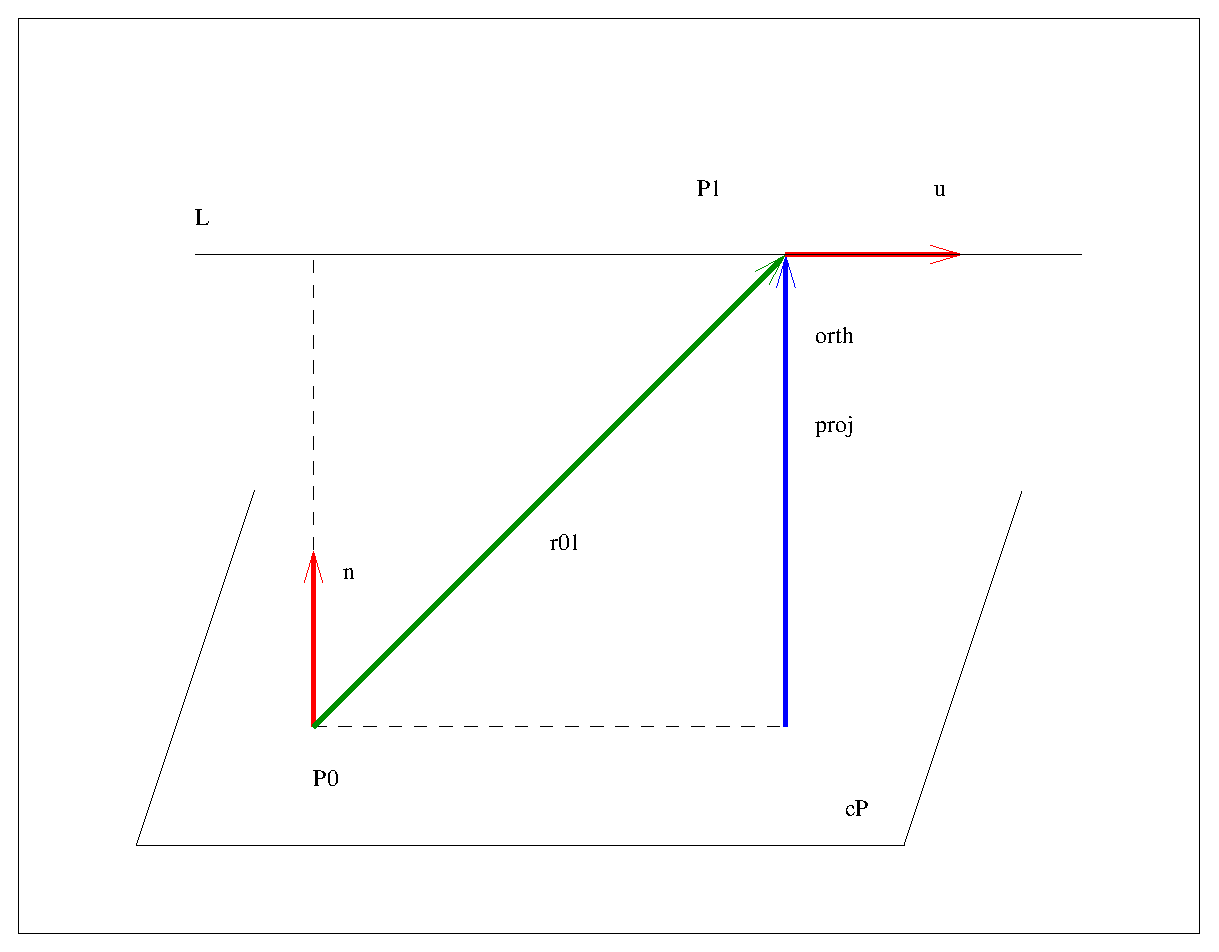
\includegraphics[height=2in]{../../modules/vectors/pictures/ok-parallel_line_plane.eps}
    \end{figure}
    %
  \end{columns}
\end{frame}

\begin{frame}
\frametitle{Angle between line and plane}
\begin{columns}
\column{0.4\textwidth}
\psset{xunit=2cm, yunit=2cm}
\begin{pspicture}(-1.2, -1.2)(2,2)
\renewcommand{\fcScreen}{[-4 -1 -1] 0}
\tiny 
\fcParallelogramIIId{[-1 -1 0]}{[1 -1 0]}{[-1 1 0]}
\fcPutIIId{[-1 1 0]}{$\mathcal P$}
\fcPerpendicularIIId[linestyle=gray]{[0.5 -0.7 0 ]}{[0 0.5 0] [0 0.5 1]}{0.2}
%\fcDotIIId{[0 0.5 1]}
%\fcPutIIId[b]{[0 0.5 1]}{$P_1(\fcv r_1)$}

\fcLineIIId[arrows=->, linecolor=blue]{[0 0.5 0]}{[0 0.5 1]}
\uncover<5>{%
\fcLineIIId[arrows=->, linewidth=2pt, linecolor=blue]{[0 0.5 0]}{[0 0.5 1]}
}%
\fcPutIIId[l]{[0 0.5 0.5]}{$~\alert<5>{\fcv{proj}_{\fcv n}(\fcv u)}$}

%\fcLineIIId[linecolor=gray]{[0.5 -0.7 0]}{[0.5 -0.7 0.9]}
\fcLineIIId[arrows=->, linecolor=red]{[0.5 -0.7 0]}{[0.5 -0.7 0.5]}
\fcPutIIId[r]{[0.5 -0.7 0.25]}{$\fcv n~~$}

\fcPerpendicularIIId[arrows=<-, linecolor=red]{[0.9 0.9 0.5]}{[0.9 0.9 0] [0.9 0.8 0]}{0.1}
\fcPutIIId[l]{[0.9 0.9 0.25]}{$~~\fcv n$}
\fcDotIIId{[0.9 0.9 0]}
\fcPutIIId[t]{[0.9 0.9 -0.1]}{$P_0(\fcv r_0)$}

\fcPutIIId{[0.5 -0.7 0]}{\fcAngleIIId {[-0.5 1.2 0]} {[-0.5 1.2 1]}{0.2}}
\uncover<4,5>{\fcPutIIId{[0.5 -0.7 0]}{\fcAngleIIId[linewidth=2pt, linecolor=red] {[-0.5 1.2 0]} {[-0.5 1.2 1]}{0.2}}}
\fcPutIIId[l]{[0.4 -0.5 0.1]}{$\alert<4,5>{ \alpha}$}

\fcLineIIId[arrows=->, linecolor=green]{[0.5 -0.7 0]}{[0 0.5 1]}
\uncover<5>{%
\fcLineIIId[arrows=->, linewidth=2pt, linecolor=green]{[0.5 -0.7 0]}{[0 0.5 1]}
}%
\fcPutIIId[tl]{[0.25 -0.1 0.5]}{$ \alert<5>{\fcv u}$}
\fcLineIIId[linestyle=dotted]{[0.56 -0.844 -0.12]}{[0.5 -0.7 0]}
\fcLineIIId{[0.65 -1.06 -0.3]}{[0.56 -0.844 -0.12]}
\fcLineIIId{[0 0.5 1]}{[-0.15 0.86 1.3]}
\fcPutIIId[tl]{[0.65 -1.06 -0.3]}{$~~L$}



\end{pspicture}
\column{0.6\textwidth}
\begin{itemize}
\item Given: line $L: \quad \fcv{r}= \fcv{r}_1+t\fcv{u}$,
\item plane $\mathcal{P}: \quad (\fcv{r}-\fcv{r}_0) \cdot \fcv{n} = 0$.
\item Goal: Find/define angle between line and plane.
\end{itemize}
\end{columns}
Line \alert<1->{perpendicular} to plane
\uncover<2->{
$\Leftrightarrow$
$\fcv{u} \| \fcv{n}$ 
\uncover<3->{%
$\Leftrightarrow$ 
$\boxed{\fcv{u} \times \fcv{n} = \fcv{0}}$
}%
}

\uncover<4->{
\alert<1->{Angle} between line and plane $\alpha$: angle between $L$, $\mathcal{P}$.
$\begin{array}{rcl}
\alert<4,5>{\sin \alpha }&\alert<4,5>{=}& \uncover<5->{\alert<5>{\frac{ \alert<6>{|\fcv{proj}_{\fcv n}\fcv u|}}{|\fcv u|} }}\uncover<6->{ = \frac{ \alert<6>{|\fcv u\cdot\fcv n|} }{ \alert<6>{|\fcv n|} |\fcv u|}}\\
\uncover<7>{ \alpha &=& \arcsin\left(\frac{|\fcv{u} \cdot \fcv{n}|}{|\fcv{u}|  |\fcv{n}|}\right) }
\end{array}
$
}
\end{frame}
\begin{frame}
  \frametitle{Parallel planes}
\begin{columns}
\column{0.4\textwidth}
\begin{pspicture}(-0.2, -0.2)(2,2)
\tiny
\fcParallelogramIIId{[-1.5 -1.5 -1]}{[-1.5 1.5 -1]}{[1.5 -1.5 -1]}
\fcParallelogramIIId{[-1.5 -1.5 1]}{[-1.5 1.5 1]}{[1.5 -1.5 1]}
\fcPutIIId{[-1.5 -1.5 -1]}{$\mathcal P_1$}
\fcPutIIId{[-1.5 -1.5 1]}{$\mathcal P_2$}
\fcLineIIId{[-1 -1 -1]}{[1 1 -1]}
\fcLineIIId{[-1 -1 1]}{[1 1 1]}
\fcDotIIId{[1 1 1]}
\fcPutIIId[tl]{[1 1 0.9]}{$~~P_2$}
\fcDotIIId{[-1 -1 -1]}
\fcPutIIId[t]{[-1 -1 -1.1]}{$P_1$}
\fcLineIIId[linecolor=gray]{[-1 -1 -1]}{[-1 -1 0.73]}%
\fcLineIIId[linecolor=gray, linestyle=dotted]{[-1 -1 0.73]}{[-1 -1 1]}%
\fcPerpendicularIIId[arrows=<-, linecolor=red]{[-1 -1 0.1]}{[-1 -1 -1] [0 0 -1]}{0.2}%
\fcPutIIId[r]{[-1 -1 -0.45]}{$\fcv n_1~~$}

\fcPerpendicularIIId[linecolor=gray]{[1 1 0.73]}{[1 1 -1] [-1 -1 -1]}{0.2}%
\fcLineIIId[linecolor=gray, linestyle=dotted]{[1 1 0.73]}{[1 1 1]}%

\fcPerpendicularIIId[arrows=<-, linecolor=red]{[1 1 1.7]}{[1 1 1] [0 0 1]}{0.2}%
\fcPutIIId[l]{[1 1 1.35]}{$~~\fcv n_2$}

\fcLineIIId[linecolor=blue]{[-1 -1 -1]}{[0.53 0.53 0.53]}
\fcLineIIId[arrows=->, linecolor=blue, linestyle=dotted]{[0.53 0.53 0.53]}{[1 1 1]}
\fcPutIIId[l]{[0 0 0]}{$~~~\fcv r_2- \fcv r_1$}
\end{pspicture}
\column{0.6\textwidth}
\begin{itemize}
\item Given: planes $\begin{array}{rrcl}
\mathcal{P}_1:& (\textbf{r} - \alert<7>{\textbf{r}_1})\alert<7>{ \cdot \alert<6>{\textbf{n}_1}} &=& 0 \\
\mathcal{P}_2:& (\textbf{r} - \alert<7>{\textbf{r}_2}) \alert<7>{\cdot \alert<6>{\textbf{n}_2}} &=& 0
\end{array}.
$
\item Goal: Establish whether planes are parallel, find distance b-n planes.
\end{itemize}
\end{columns}
Planes are \alert<1->{parallel} \uncover<2->{$\mathcal{P}_1 || \mathcal{P}_2$ $\Leftrightarrow$ $\textbf{n}_1$, $\textbf{n}_2$ collinear $\Leftrightarrow$
$\boxed{\textbf{n}_1 \times \textbf{n}_2 = \textbf{0}}$. }

\uncover<3->{\alert<1->{Distance}:\quad
$d(\mathcal{P}_1,\mathcal{P}_2) = |\textbf{\text{proj}}_{\textbf{n}_1} (\textbf{r}_2-\textbf{r}_1)| \uncover<4->{=\boxed{\frac{|(\textbf{r}_2-\textbf{r}_1)\cdot \textbf{n}_1|}{|\textbf{n}_1|}}}$
} %uncover3

\uncover<5->{%
\noindent Assume $\alert<6>{ \fcv n_1=\fcv n_2=( a,b,c) }$
\uncover<6->{$\Rightarrow$ plane eq-ns:
$\begin{array}{r@{~}r@{~}c@{~}l}
\mathcal{P}_1 :& \alert<6>{a}x+\alert<6>{b}y+\alert<6>{c}z &=& \alert<7>{d_1}\\
\mathcal{P}_2 :& \alert<6>{a}x+\alert<6>{b}y+\alert<6>{c}z &=& \alert<7>{d_2}
\end{array}.$
}
\uncover<7->{
\[
\Rightarrow \boxed{d(\mathcal{P}_1,\mathcal{P}_2) = \frac{|\alert<7>{d_2-d_1}|}{\sqrt{a^2+b^2+c^2}}}
\]
}
}%uncover5
\end{frame}

\begin{frame}
\frametitle{Angle between planes}
\begin{columns}
\column{0.35\textwidth}
\centering
\psset{xunit=1.2cm, yunit=1.2cm}
\begin{pspicture}(-2, -2.5)(2,1.4)
\tiny
\renewcommand{\fcScreenStyle}{x}
%\fcAxesIIId{2}{2}{2}
\fcParallelogramIIId[linecolor=green!30]{[1 0 -1]}{[1 1 -1]}{[0 0 0]}
\fcParallelogramIIId[linecolor=magenta!30]{[1 0 0]}{[1 1 0]}{[-1 0 0]}
\fcParallelogramIIId[linecolor=green!30]{[0 0 0]}{[-1 0 1]}{[0 1 0]}
\uncover<6->{
\fcParallelogramIIId[linecolor=cyan!30]{[1 0 -1]}{[1 0 1]}{[-1 0 -1]}
}
\fcParallelogramIIId[linecolor=green!30]{[1 -1 -1]}{[1 0 -1]}{[0 -1 0]}
\fcParallelogramIIId[linecolor=magenta!30]{[1 -1 0]}{[1 0 0]}{[-1 -1 0]}
\fcParallelogramIIId[linecolor=green!30]{[0 0 0]}{[0 -1 0]}{[-1 0 1]}

\uncover<6->{%
\fcPutIIId[b]{[0.8 0 1.1]}{$\mathcal P_3$}
\fcPolyLineIIId{[1 0 -1] [1 0 1] [-1 0 1]}
\fcLineIIId[linestyle=dashed]{[-1 0 1]}{[-1 0 -0.5]}
\fcPolyLineIIId{[-1 0 -0.5] [-1 0 -1] [-0.5 0 -1]}
\fcLineIIId[linestyle=dashed]{[-0.5 0 -1]}{[1 0 -1]}
}
\fcPolyLineIIId[linestyle=dashed]{[-1 -0.35 0] [-1 1 0] [0 1 0]}
\fcPolyLineIIId{[-1 -0.35 0] [-1 -1 0] [1 -1 0] [1 1 0] [0 1 0]}
\fcPolyLineIIId{[0 1 0] [-1 1 1] [-1 -1 1] [1 -1 -1] [1 1 -1] [0.33 1 -0.33]}%
\fcLineIIId[linestyle=dashed]{[0.33 1 -0.33]}{[0 1 0]}%
%\uncover<9->{%
%\fcPerpendicularIIId[arrows=<-, linecolor=red]{[1.7 0 0.3]}{[1 0 -1]}{0.2}%
%\fcDotIIId{[0.7 0 -0.7]}%
%\fcPutIIId[tl]{[0.7 0 -0.7]}{$~~P_1$}%
%\fcPutIIId[l]{[1.5 0 0]}{$~\fcv n_1$}
%}%
%\fcPerpendicularIIId[arrows=<-, linecolor=red]{[1 0 1]}{[-1 0 1]}{0.2}
\uncover<9->{%
\fcLineIIId[arrows=<-, linecolor=red]{[1 0 1]}{[0 0 0]}
\fcPutIIId[tl]{[0.85 0 0.85]}{$~~~~\fcv n_1$}%
}%
%\uncover<9->{%
%\fcPerpendicularIIId[arrows=<-, linecolor=red]{[0.8 0.8 0.8]}{[0.8 0.8 0] [0.6 0.8 0]}{0.2}%
%\fcDotIIId{[0.8 0.8 0]}
%\fcPutIIId[bl]{[0.8 0.8 0]}{$~~P_2$}
%\fcPutIIId[bl]{[0.8 0.8 0.5]}{$~~\fcv n_2$}
%}%

\fcLineIIId[linecolor=gray]{[0 -1 0]}{[0 1 0]}
\fcPutIIId[b]{[0 -1 0.1]}{$L$}
%\fcPerpendicularIIId[arrows=<-, linecolor=red]{[0 0 0.8]}{[-1 0 0]}{0.1}
\uncover<9->{%
\fcLineIIId[arrows=<-, linecolor=red]{[0 0 0.8]}{[0 0 0]}
\fcPutIIId[bl]{[0 0 0.5]}{$~~\fcv n_2$}
}%
\fcPolyLineIIId{[-0.5 0 0.5] [0 0 0]}%
\fcLineIIId[linestyle=dashed]{[0 0 0]}{[0.2 0 -0.2]}%
\uncover<3-4>{%
\fcPerpendicularIIId{[-0.5 0 0.5]}{[0 1 0]}{0.2}%
}%
\uncover<3->{%
\fcDotIIId{[-0.5 0 0.5]}%
\fcPutIIId[b]{[-0.5 0 0.6]}{$Q_1$}
}%

\fcLineIIId[linestyle=dashed]{[0 0 0]}{[-0.7 0 0]}%
\fcLineIIId{[0 0 0]}{[0.7 0 0]}%
\uncover<4->{%
\fcDotIIId{[-0.7 0 0]}%
\fcPutIIId[t]{[-0.7 0 -0.1]}{$Q_2$}
}%
\uncover<4>{%
\fcPerpendicularIIId[linestyle=dashed]{[-0.7 0 0]}{[0 1 0]}{0.2}%
}%
\uncover<5->{%
\fcAngleIIId[linecolor=blue]{[-1 0 1]}{[-1 0 0]}{0.3}%
\fcPutIIId[rb]{[-0.3 0 0.1]}{$\alpha$}%
}%
\uncover<11->{\fcAngleIIId[linecolor=blue]{[0 0 1]}{[1 0 1]}{0.3}}%
\uncover<13->{%
\fcLineIIId[arrows=->, linecolor=blue]{[0 0 0]}{[0 -0.8 0]}%
\fcPutIIId[l]{[0 -0.5 0]}{$~\fcv u$}%
}%
\fcPutIIId[tr]{[-1 -1 0]}{$\mathcal P_2$}
\fcPutIIId[tr]{[-1 -1 1]}{$\mathcal P_1$}
%\fcParallelogramHollowIIId{[-1 -1 0]}{[1 -1 0]}{[-1 1 0]}
%\fcParallelogramHollowIIId{[1 -1 -1]}{[1 1 -1]}{[-1 -1 1]}
\end{pspicture}
\uncover<6->{%
\psset{xunit=1cm, yunit=1cm}
\begin{pspicture}(-1.2, -1.2)(1.2, 1.4)
\tiny
\renewcommand{\fcScreen}{[0 1 0] 0}
\fcBoundingBox{-1.5}{-1.5}{1.5}{1.5}
\fcParallelogramIIId[linecolor=cyan!30]{[1 0 -1]}{[1 0 1]}{[-1 0 -1]}
\fcPutIIId[t]{[0 0 -0.1]}{$O$}
\fcPutIIId[b]{[0.8 0 1.1]}{$\mathcal P_3$}
\uncover<9->{%
\fcPutIIId[bl]{[0 0 0.6]}{$~~\fcv n_2$}
\fcPutIIId[tl]{[0.85 0 0.85]}{$~~\fcv n_1$}%
}%uncover9
\uncover<9>{%
\fcLineIIId[arrows=<-, linecolor=red]{[0 0 0.8]}{[0 0 0]}%
\fcLineIIId[arrows=<-, linecolor=red]{[1 0 1]}{[0 0 0]}%
}%uncover9
\uncover<10->{%
\fcPerpendicularIIId[arrows=<-, linecolor=red]{[0 0 0.8]}{[1 0 0]}{0.12}%
\fcPerpendicularIIId[arrows=<-, linecolor=red]{[1 0 1]}{[1 0 -1]}{0.2}%
}%
\fcLineIIId{[0 0 0]}{[-0.7 0 0]}%
\fcPolyLineIIId{[-0.5 0 0.5] [0 0 0]}%
\fcAngleIIId[linecolor=blue]{[-1 0 1]}{[-1 0 0]}{0.35}%
\fcPutIIId[rb]{[-0.3 0 0.15]}{$\alpha$}%
\uncover<11->{%
\fcAngleIIId[linecolor=blue]{[0 0 1]}{[1 0 1]}{0.35}%
\fcPutIIId[lb]{[0.1 0 0.35]}{$\alpha~~$}%
}%
\fcDotIIId{[-0.5 0 0.5]}%
\fcPutIIId[b]{[-0.5 0 0.6]}{$Q_1$}
\fcDotIIId{[-0.7 0 0]}%
\fcPutIIId[t]{[-0.7 0 -0.1]}{$Q_2$}
\end{pspicture}
}%
\vskip 6cm
\column{0.65\textwidth}
\begin{itemize}
\item Given: planes 
$\begin{array}{rrcl}
\mathcal{P}_1:&  (\fcv{r} - \fcv{r}_1) \cdot \alert<9>{\fcv{n}_1 }&=& 0 \\
\mathcal{P}_2:& (\fcv{r} - \fcv{r}_2) \cdot \alert<9>{\fcv{n}_2} &=& 0
\end{array}
$
\item Goal: \alert<4>{define} and find the angle between the two planes.
\only<handout:1| 1-6>{%
\item<2-> Let $L$ - intersection line of two planes.
\item<3-> In $\mathcal P_1$, drop perpendicular from arbitrary point $Q_1$ to $L$.
\item<4-> In $\mathcal P_2$, raise a perpendicular from the perpendicular heel.
\item<5-> \alert<4>{Define angle $\alpha$} b-n $\mathcal P_1, \mathcal P_2$ = acute angle b-n two perpendiculars.
}%
\item<6-> \alert<6,7>{Consider the plane $\mathcal P_3$ spanned by the two constructed perpendiculars.}

\only<handout:1| 1-6>{%
\vskip 0.57cm
}%
\only<handout: 2| 7->{%
\item<8-> $\mathcal P_3$ is orthogonal to $L$.
\item<9-> $\Rightarrow$ $\mathcal P_3$ contains the normal vectors $\fcv n_1$, $\fcv n_2$.
\item<10-> $\fcv n_1\perp \fcv O\fcv Q_{1}$ and $\fcv n_2\perp \fcv O\fcv Q_{2}$.
\item<11-> 
$
\begin{array}{rcl}
\alpha &=& \text{acute} \angle (\fcv{n}_1,\fcv{n}_2) \\
\alpha &=&\arccos{\left( \frac{|\fcv{n}_1 \cdot \fcv{n}_2|}{|\fcv{n}_1|\, |\fcv{n}_2|}\right)}
\end{array}
$
\item<12-> $\perp$ planes: $\Rightarrow$ $\alpha = \frac{\pi}{2} \Longleftrightarrow \boxed{\fcv{n}_1 \cdot \fcv{n}_2 = 0}$.
\item<13-> Direction of $L$ is $\fcv{u} = \fcv{n}_1 \times \fcv{n}_2$.
}%onlyr<7->
\end{itemize}

\vfill

\end{columns}
\vskip 5cm

\end{frame}
} %end lecture


% begin lecture

%\section{(Appendix G) Complex Numbers}
% WARNING:  Appendix G is missing here.
% end lecture
\end{document}
